\documentclass[]{article}
\usepackage{lmodern}
\usepackage{color}
\usepackage{amssymb,amsmath}
\usepackage{ifxetex,ifluatex}
\usepackage{fixltx2e} % provides \textsubscript
\ifnum 0\ifxetex 1\fi\ifluatex 1\fi=0 % if pdftex
  \usepackage[T1]{fontenc}
  \usepackage[utf8]{inputenc}
\else % if luatex or xelatex
  \ifxetex
    \usepackage{mathspec}
    \usepackage{xltxtra,xunicode}
  \else
    \usepackage{fontspec}
  \fi
  \defaultfontfeatures{Mapping=tex-text,Scale=MatchLowercase}
  \newcommand{\euro}{€}
\fi
% use upquote if available, for straight quotes in verbatim environments
\IfFileExists{upquote.sty}{\usepackage{upquote}}{}
% use microtype if available
\IfFileExists{microtype.sty}{%
\usepackage{microtype}
\UseMicrotypeSet[protrusion]{basicmath} % disable protrusion for tt fonts
}{}
\usepackage[margin=1.5in]{geometry}
\usepackage{longtable,booktabs}
\usepackage{graphicx}
\makeatletter
\def\maxwidth{\ifdim\Gin@nat@width>\linewidth\linewidth\else\Gin@nat@width\fi}
\def\maxheight{\ifdim\Gin@nat@height>\textheight\textheight\else\Gin@nat@height\fi}
\makeatother
% Scale images if necessary, so that they will not overflow the page
% margins by default, and it is still possible to overwrite the defaults
% using explicit options in \includegraphics[width, height, ...]{}
\setkeys{Gin}{width=\maxwidth,height=\maxheight,keepaspectratio}
\ifxetex
  \usepackage[setpagesize=false, % page size defined by xetex
              unicode=false, % unicode breaks when used with xetex
              xetex]{hyperref}
\else
  \usepackage[unicode=true]{hyperref}
\fi
\hypersetup{breaklinks=true,
            bookmarks=true,
            pdfauthor={},
            pdftitle={},
            colorlinks=true,
            citecolor=blue,
            urlcolor=blue,
            linkcolor=magenta,
            pdfborder={0 0 0}}
\urlstyle{same}  % don't use monospace font for urls
\setlength{\parindent}{0pt}
\setlength{\parskip}{6pt plus 2pt minus 1pt}
\setlength{\emergencystretch}{3em}  % prevent overfull lines
\setcounter{secnumdepth}{0}

\date{}
\usepackage{lineno}
\linenumbers
\usepackage{setspace}
\doublespacing
\definecolor[blue][r=.25, g = .1, b=1]

\begin{document}

\section{GLO-Roots: an imaging platform enabling multidimensional
characterization of soil-grown roots
systems}\label{glo-roots-an-imaging-platform-enabling-multidimensional-characterization-of-soil-grown-roots-systems}

Rubén Rellán-Álvarez\textsuperscript{1,~9}, Guillaume
Lobet\textsuperscript{2}, Heike Lindner\textsuperscript{1,~8},
Pierre-Luc Pradier\textsuperscript{1,~8,~10}, Jose
Sebastian\textsuperscript{1,~8}, Muh-Ching Yee\textsuperscript{1}, Yu
Geng\textsuperscript{1,~7}, Charlotte Trontin\textsuperscript{1},
Therese LaRue\textsuperscript{3}, Amanda
Schrager-Lavelle\textsuperscript{4}, Cara H. Haney\textsuperscript{5},
Rita Nieu\textsuperscript{6}, Julin Maloof\textsuperscript{4}, John P.
Vogel\textsuperscript{7}, José R. Dinneny\textsuperscript{1,~12}

\textsuperscript{1} Department of Plant Biology, Carnegie Institution
for Science, Stanford, CA, USA.

\textsuperscript{2} PhytoSystems, University of Liège, Liège, Belgium.

\textsuperscript{3} Department of Biology, Stanford University,
Stanford, CA, USA.

\textsuperscript{4} Department of Plant Biology, UC Davis, Davis, CA,
USA.

\textsuperscript{5} Harvard Medical School, Massachusetts General
Hospital, Department of Genetics, Department of Molecular Biology
Boston, MA, USA

\textsuperscript{6} USDA Western Regional Research Center, Albany, CA,
USA

\textsuperscript{7} DOE Joint Genome Institute, Walnut Creek, CA, USA

\textsuperscript{8} These authors contributed equally

\textsuperscript{9} Present address: Laboratorio Nacional de Genómica
para la Biodiversidad (Langebio), Unidad de Genómica Avanzada, Centro de
Investigación y de Estudios Avanzados del Instituto Politécnico Nacional
(CINVESTAV-IPN), Irapuato, Guanajuato, México

\textsuperscript{10} Present address: Boyce Thompson Institute for Plant
Research/USDA, Ithaca, NY, USA.

\textsuperscript{11} Present address: Energy Biosciences Institute, UC,
Berkeley, CA, USA

\textsuperscript{12} Corresponding author

\textbf{Author contributions:}

RR-A: Conception, design and development of the growth and imaging
system and Arabidopsis transgenic lines; acquisition, analysis and
interpretation of data; drafting and revising the article.

GL: Development of the GLO-RIA image analysis plugin, analysis and
interpretation of data, drafting and revising the article.

HL: Acquisition of data, development of the tomato growth and imaging
setup.

P-LP: Acquisition of data, analysis and interpretation of data

JS: Development of Brachypodium transgenic lines, acquisition and
analysis of Brachypodium, Arabidopsis and tomato data.

MCY: Development of Arabidopsis and Brachypodium transgenic lines.

YG: Development of Arabidopsis transgenic lines.

CT: Acquisition and analysis of the QPCR data

TL: Acquisition and analysis of the QPCR data

AS-L: Contributed the unpublished dual-color tomato line.

CH: Contributed the unpublished \emph{Pseudomonas fluorescens} CH267-lux
strain.

RN: Contribution to the development of the Brachypodium transgenic line.

JM: Contributed the unpublished dual-color tomato line.

JPV: Contribution to the development of the Brachypodium transgenic
line.

JRD: Conception, design and development of the growth and imaging system
and Arabidopsis transgenic lines; acquisition, analysis and
interpretation of data; drafting and revising the article.

All authors read and approve the final version of the manuscript.

\subsection{Abstract}\label{abstract}

Root systems develop different root types that individually sense cues
from their local environment and integrate this information with
systemic signals. This complex multi-dimensional amalgam of inputs
enables continuous adjustment of root growth rates, direction and
metabolic activity that define a dynamic physical network. Current
methods for analyzing root biology balance physiological relevance with
imaging capability. To bridge this divide, we developed an integrated
imaging system called Growth and Luminescence Observatory for Roots
(GLO-Roots) that uses luminescence-based reporters to enable studies of
root architecture and gene expression patterns in soil-grown,
light-shielded roots. We have developed image analysis algorithms that
allow the spatial integration of soil properties such as soil moisture
with root traits. We propose GLO-Roots as a system that has great
utility in presenting environmental stimuli to roots in ways that evoke
natural adaptive responses and in providing tools for studying the
multi-dimensional nature of such processes.

\subsection{Introduction}\label{introduction}

Plant roots are three-dimensional assemblies of cells that coordinately
monitor and acclimate to soil environmental change by altering
physiological and developmental processes through cell-type and
organ-specific regulatory mechanisms\textsuperscript{1,2}. Soil
comprises a complex distribution of particles of different size,
composition and physical properties, airspaces, variation in nutrient
availability and microbial diversity\textsuperscript{3,4}. These
physical, chemical and biological properties of soil can vary on spatial
scales of meters to microns, and on temporal scales ranging from
seasonal change to seconds. Root tips monitor this environment through
locally and systemically acting sensory mechanisms\textsuperscript{5,6}.

The architecture of the root system determines the volume of soil where
resources can be accessed by the plant (rhizosphere) and is under both
environmental and genetic control. Plasticity in growth parameters
allows the plant to adjust its form to suit a particular soil. Lateral
roots, which usually make up the majority of the total root system,
often grow at an angle divergent from the gravity vector. This gravity
set-point angle (GSA) is controlled by auxin biosynthesis and signaling
and can be regulated by developmental age and root
type\textsuperscript{7}. Recent cloning of the \emph{DRO1} Quantitative
Trait Locus (QTL) demonstrates that natural genetic variation is a
powerful tool for uncovering such control mechanisms\textsuperscript{8}.

Specific root ideotypes (idealized phenotypes) have been proposed to be
optimal for acquisition of water and nitrogen, which are distinct from
ideotypes for low phosphorus. Based on computational modeling and field
studies, the ``steep, deep and cheap'' ideotype proposed by Lynch and
colleagues may provide advantages to the plant for capturing water and
elements like nitrogen that are water soluble and therefore tend to move
in the soil column with water. This ideotype consists of highly
gravitropic, vertically oriented roots that grow deep in the soil column
and develop large amounts of aerenchyma, which reduces the overall
metabolic cost of the root system\textsuperscript{3}. Other nutrients,
like phosphorus, which have limited water solubility and are tightly
bound to organic matter, usually accumulate in the top layers of soil
and favor roots systems that are more highly branched and shallow. The
low-phosphorus ideotype effectively increases root exploration at the
top layers of soil\textsuperscript{3}. Modeling of root system variables
shows that optimum architecture for nitrogen and phosphorus uptake are
not the same\textsuperscript{9} and suggests tradeoffs that may affect
the evolution of root architecture as a population adapts to a
particular environmental niche.

Clearly, understanding the architecture of root systems and how
environmental conditions alter root developmental programs is important
for understanding adaptive mechanisms of plants and for identifying the
molecular-genetic basis for different response programs. In addition,
roots systems have complexity beyond their architecture that needs to be
incorporated into our understanding of plant-environment interactions.
Primary and lateral roots exhibit different stress response programs in
Arabidopsis\textsuperscript{2} and may play specialized roles in water
and nutrient uptake. Thus, it is important to develop methods that allow
for a multidimensional characterization of the root system that includes
growth, signaling, and interactions with other organisms. Furthermore,
physiological parameters that affect whole plant responses to the
environment, such as transpiration, are likely integrated into such
processes, thus requiring a more holistic approach to studies of root
function.

Based on these considerations we have developed a new root imaging
platform, Growth and Luminescence Observatory for Roots (GLO-Roots),
which allows root architecture and gene expression to be studied in
soil-grown plants. GLO-Roots is an integrated system composed of custom
growth vessels, luminescent reporters and imaging systems. We use
rhizotrons that have soil volumes equivalent to small pots and support
growth of Arabidopsis from germination to senescence. To visualize
roots, we designed plant-codon optimized luciferase reporters that emit
light of different wavelengths. To visualize reporter expression, plants
are watered with a dilute luciferin solution and imaged afterwards. We
have built a custom luminescence imaging system that automatically
captures images of rhizotrons held vertically. The signal from each
reporter is distinguished using band-pass filters held in a motorized
filter wheel, which enables automated acquisition of images from plants
expressing both structural and environmentally and developmentally
responsive reporters. We have also developed GLO-RIA (GLO-Roots Image
Analysis), an ImageJ\textsuperscript{10} plugin that allows for
automated determination of root system area, convex hull, depth, width
and directionality, which quantifies the angle of root segments with
respect to gravity. GLO-RIA is also able to relate root system
parameters to local root-associated variables such as reporter
expression intensity and soil-moisture content.

Overall GLO-Roots has great utility in presenting environmental stimuli
to roots in physiologically relevant ways and provides tools for
characterizing responses to such stimuli at the molecular level in whole
adult root systems over broad time scales.

\subsection{Box 1.}\label{box-1.}

All resources for GLO-Roots, including the original raw data used in the
manuscript, sample images, GLO-RIA user manual, the latest software
updates and the source code, can be found at:
https://dinnenylab.wordpress.com/glo-roots/

\subsection{Results}\label{results}

We have developed an integrated platform for growing, imaging and
analyzing root growth that provides advances in physiological relevance
and retains the ability to visualize aspects of root biology beyond
structure.

\subsubsection{The GLO-Roots plattform}\label{the-glo-roots-plattform}

GLO-Roots is comprised of four parts: i) growth vessels called
rhizotrons that allow plant growth in soil and root imaging; ii)
luminescent reporters that allow various aspects of root biology to be
tracked in living plants; iii) GLO1 luminescence-imaging system designed
to automatically image rhizotrons; iv) GLO-RIA, an image analysis suite
designed to quantify root systems imaged using GLO-Roots.

\paragraph{Plant growth system}\label{plant-growth-system}

GLO-Roots utilizes custom designed growth vessels classically known as
rhizotrons, which hold a thin volume of soil between two sheets of
polycarbonate plastic. Acrylic spacers provide a 2-mm space in which
standard peat-based potting mix is added. Black vinyl sheets protect
roots from light and rubber U-channels clamp the rhizotron materials
together. Plastic racks hold the rhizotrons vertically and further
protect the roots from light. Rhizotrons and rack are placed in a black
tub and water are added, to a depth of about 2 cm, at the bottom to
maintain moisture in the rhizotrons during plant growth. The volume of
soil in the rhizotrons (100 cm\textsuperscript{3}) is similar to small
pots commonly used for Arabidopsis and supports growth throughout the
entire life cycle (Fig 1A-C and Supplement 1). To determine how the
biology of plants grown in rhizotrons compares to other standard growth
systems, we utilized high-throughput qRT-PCR to study how these
conditions affect expression of 77 marker genes in root and shoot
samples. These genes were curated from the literature and belong to a
wide array of biological pathways including nutrient acquisition,
hormone and light response and abiotic stress. Whole roots and shoot
samples were collected at the end of the light and dark periods
(Long-day conditions: 16 hour light, 8 hours dark) from plants grown in
rhizotrons, pots, and petri dishes with two different media compositions
(1X Murashige and Skoog basal salts (MS), 1\% sucrose or 0.25X MS, no
sucrose). Principal component analysis of the gene expression values
showed a separation of soil and gel-grown root systems in the the first
principal components (Figure 1-figure supplement 1A). In roots grown on
gel-based media, we observed enhanced expression of genes associated
with light-regulated pathways (flavonoid biosynthesis: \emph{FLAVINOL
SYNTHASE1, FLS1}, \emph{CHALCONE SYNTHASE, CHS} and photosynthesis:
\emph{RUBSICO SUBUNITS1A, RBCS1A}, \emph{CYCLOPHILIN 38, CYP38}), which
is expected due to the exposure of gel-grown roots to light. In
addition, genes associated with phosphorus nutrition (\emph{LOW
PHOSPHATE RESPONSE1}, \emph{LPR1, PHOSPHATE STARVATION RESPONSE1, PHR1})
were (Figure 1-figure table supplement 1) less expressed in soil-grown
roots, suggesting differences in nutrient availability between the
different growth systems. Interestingly, shoot samples where not clearly
distinguished by growth media and, instead, time of day had a greater
effect (Figure 1-Supplement 2). These data suggest root systems may be
particularly sensitive to media conditions and indicate that
rhizotron-grown root systems more closely approximate the biology of
pot-grown plants than standard gel-based media. Shoot weight and primary
root length were significantly reduced for gel-grown plants compared to
rhizotron- or pot-grown plants suggesting significant differences in the
biology of plants grown under these conditions (Figure 1-figure
supplement 1B-C). While the 2 mm depth of the soil sheet is 10 to 20
times the average diameter of an Arabidopsis root (between 100-200
microns\textsuperscript{11}), we evaluated whether rhizotron-grown
plants exhibited any obvious stress as a consequence of physical
constriction. We compared traits of plants growing in vessels that hold
similar volumes of soil but in different volumetric shapes. The number
of lateral roots was significantly lower in pot and cylinder-grown
plants compared to rhizotron-grown plants (Figure 1-figure supplement
1D) whereas primary root length of rhizotron and cylinder-grown plants
was significantly greater than pot-grown plants (Figure 1-figure
supplement 1E). No significant differences in shoot area were observed
between the three systems (Figure 1-figure supplement 1-data). Thus,
these data do not support the hypothesis that rhizotron-grown plants
experience physical constriction greater than other vessels holding the
same volume of soil.

\paragraph{Generation of transgenic plants expressing different
luciferases}\label{generation-of-transgenic-plants-expressing-different-luciferases}

Arabidopsis roots cannot easily be distinguished from soil using
brightfield imaging due to their thinness and translucency (Figure
1-figure supplement 3); thus, reporter genes are needed to enhance the
contrast between the root and their environment. Luciferase is an ideal
reporter to visualize roots: 1) unlike fluorescent reporters, luciferase
does not require high-intensity excitation light, which could influence
root growth, 2) peat-based soil (a type of histosol) exhibits no
autoluminescence but does autofluoresce at certain excitation
wavelengths similar to GFP (Figure 1-figure supplement 3), 3) while GFP
is very stable, and thus not as suitable for imaging dynamic
transcriptional events, the luciferase enzyme is inactivated after
catabolism of luciferin, making it ideal for studying processes such as
environmental responses. A considerable number of luciferases have been
developed that emit light spanning different regions of the visible
spectrum, but their utilization has been limited to studies in animals
(Table 1).

To determine the efficacy of using luciferase to visualize roots in
soil, we codon optimized sequences of \emph{PpyRE8}, \emph{CBGRed},
\emph{LUC2}, and \emph{CBG99} for Arabidopsis expression. In addition,
nanoLUC and venus-LUC2\textsuperscript{12} were utilized. Constitutive
luciferase expression was driven in plants using the \emph{UBIQUITIN 10
(UBQ10)} or \emph{ACTIN2 (ACT2)} promoters using vectors assembled
through a Golden-Gate cloning system\textsuperscript{13}. Plants
homozygous for a single locus T-DNA insertion were evaluated for in vivo
emission spectra and luminescence intensity (Fig 1D). All the evaluated
luciferases use D-luciferin as a substrate facilitating the simultaneous
imaging of different luciferases except nanoLUC, which uses a
proprietary substrate furimazine\textsuperscript{14}. In general,
luciferases with red-shifted emission spectra were less intense than the
green-shifted luciferases (Fig 1D). LUC2o showed an emission maximum at
580 nm and a minor peak at 620 nm while CBG99o lacks the minor peak.

Continuous addition of luciferin did not have any significant effect on
shoot weight or primary root length (Figure 1-figure supplement 4).
After luciferin addition, luminescence signal could be reliably detected
in root systems for up to 10 days, depending on the developmental state
of the plant.

\paragraph{GLO1: a semi-automated luminescence imaging system for
rhizotrons}\label{glo1-a-semi-automated-luminescence-imaging-system-for-rhizotrons}

Luminescence imaging systems commercially available for biomedical
research are usually optimized for imaging horizontally held specimens
or samples in microtiter plates. Placing rhizotrons in this position
would induce a gravitropic response in plants. Working with Bioimaging
Solutions (San Diego, CA) we designed and built a luminescence imaging
system optimized for rhizotron-grown plants. GLO1 (Growth and
Luminescence Observatory 1) uses two back-thinned CCD cameras (Princeton
Instruments, USA) to capture partially-overlapping images of rhizotrons
while a motorized stage automatically rotates the rhizotron to capture
images of both sides (Fig 1E). A composite image is generated from the
images captured of each side; Fig 1F shows that approximately half of
the root system is revealed on each side with few roots being visible on
both sides. Apparently, the soil sheet is thick enough to block portions
of the root system but thin enough to ensure its continuous structure
can be compiled from opposite face views. We tested the ability of
GLO1-generated images to reveal complete root systems by manually
quantifying the number of lateral roots in excavated root systems of 8
different plants and testing these results against estimates of lateral
root number from images of the same plants visually inspected by 4
different persons. These comparisons revealed good correlation
((R\textsuperscript{2}= 0.974)) between actual lateral root counts and
image-based estimation, indicating GLO1-generated root images provide an
accurate representation of the in soil root system.

\paragraph{\texorpdfstring{\href{https://github.com/rr-lab/GLO-Roots/blob/master/gloria/GLORIA/manual/GLO_RIA_manual.md}{GLO-RIA}:
GLO-Roots Image
Analysis}{GLO-RIA: GLO-Roots Image Analysis}}\label{glo-ria-glo-roots-image-analysis}

We developed a set of image analysis algorithms that were well suited
for the complex root systems that GLO-Roots is able to capture. GLO-RIA
(Growth and Luminescence Observatory Root Image Analysis) is an ImageJ
plugin divided in two modules. The first module (RootSystem) performs
four different types of analysis: i) a local analysis that detects all
root particles in the image and computes their position, length and
direction; ii) the global analysis performs a root system level analysis
and computes the total visible surface, convex hull, width and depth;
iii) the shape analysis uses Elliptic Fourier Descriptors or
pseudo-landmarks similarly to RootScape\textsuperscript{15} to perform a
shape analysis on the root system iv) the directionality analysis
computes the mean direction of root particles in a root system (either
on the full image or by a user-defined region of interest in the image).
These four analysis methods are fully automated by default, but can be
manually adjusted if needed. The second module of GLO-RIA (RootReporter)
was specifically designed for the analysis of multi-layered images such
as combinations of gene reporter, root structure and soil moisture.
Shortly, the plugin works as follows: i) detection of the gene reporters
and the structure reporters in their respective images; ii) if needed, a
manual correction can be performed to correct the automated detection;
iii) gene reporters are linked with the soil water content and the
structure reporters, based on their proximity; iv) gene reporter
intensity (either absolute or normalized using the structural reporter)
is computed; v) all data are exported and saved to a RSML
datafile\textsuperscript{16}. Gene and structure reporters can be
followed across different time and space points. Using an object
oriented approach, great care has been taken to facilitate the user
interactions on the different images to streamline the analysis process.
Table 2 shows a list of root system features extracted using GLO-RIA.
GLO-RIA does not currently have the ability to reconstruct the root
architecture in itself (topological links between roots). This is a
challenge for analyzing images captured by GLO-Roots since soil
particles cause disruption of root segments. \color{blue}{We validated the
measurements obtained with GLO-RIA using two approaches}. First, we
compared the root system width, depth and individual lateral root angles
of an indepent set of images corresponding to different Arabidopsis
accesions growing in control conditions with the the the width, depth
and root system directionality obtained with GLO\_RIA. Since the root
system width and depth can be manually corrected in GLO-RIA we obtained
almost perfect correlation for this measurements (Figure 1-figure
supplement 5A,B). We also obtained good correlations for the
directionality and the mean lateral root angles measured by GLO-RIA
(Figure 1-figure supplement 5C), showing that the directionality is a
good estimator of the mean lateral root angle of a root system. We then
used ArchiSimple\textsuperscript{17} to generate 1240 images with
contrasting sizes and lateral root angles. Since the images are
generated by the model, we can obtain very precise ground truth
measurements that we then used to validate the GLO-RIA obtained values
for the same parameters (depth, width and directionality). Again, we
obtained good correlations for all three measured parameters (Figure
1-figure supplement 5D-F). Sample images of the real root systems and
ArchiSimple generated images together with GLO-RIA directionality
color-coded images are also shown in (Figure 1-figure supplement 5G-I).

\subsubsection{Continuous imaging of root
growth}\label{continuous-imaging-of-root-growth}

The size of our rhizotrons enables undisturbed root system development
(before roots reach the sides or the bottom of the rhizotron) for about
21-23 days for the Col-0 accession growing under long day conditions
(Figure 2); however root traits such as directionality can be observed
through later stages of plant development. See 35 DAS root system and
directionality in Figure 2A-B. An example of a time series spanning 11
to 21 days after sowing (DAS) of Col-0 roots expressing
\emph{ProUBQ10:LUC2o} is shown in Fig 2A and
\href{https://www.dropbox.com/s/sxjc04o0yj2faif/Video_1.avi?dl=0}{Video
1} with a color-coded time projection shown in Fig 2C. Directionality
analysis (Fig 2B) shows a progressive change in root system angles from
0 º (vertical) to 45 º as lateral roots take over as the predominant
root type. Figure 2D shows the evolution over time of several root
traits that can be automatically captured by GLO-RIA (depth, width,
area) and others that were manually quantified (primary root growth rate
or number of lateral roots per primary root).\\\#\#\# Root system
architecture of different Arabidopsis accessions.

As a proof of concept to estimate the utility of our root imaging system
to phenotype adult root system traits, we transformed a small set of
accessions (Bay-0, Col-0 and Sha) with the \emph{ProUBQ10:LUC2o}
reporter and quantified RSA at 22 DAS (Fig 3A-C). GLO-RIA analysis of
these root systems identified several root traits that distinguish
Col-0, Bay-0 and Sha. Directionality analysis revealed an abundance of
steep-angle regions in the root system of Bay while Sha showed an
abundance of shallow-angled regions and Col-0 was intermediate (Fig 3D).
Bay-0 shows the deepest and narrowest root system leading to the highest
depth/width ratio while Sha has the widest root system (Fig 3E). Other
root traits such as root system area and the vertical center of mass
also showed significant differences (Figure 3-figure supplement 1B).
Broad sense heritability values for depth (96.3), area (92.0),
depth/width (97.8), width (95.7) and vertical center of mass (95.0) were
all higher than 90\%.\\ To capture the richness of root architecture
shape, we used GLO-RIA to extract pseudo-landmarks describing the shape
of the root system (see Materials and Methods for more details) and
performed PCA analysis. The first principal component captures
differences in the distribution of widths along the vertical axis and
separates Col-0 and Sha from Bay-0 root systems. (Fig 3F). Bay-0 shows
an homogenous distribution of widths along the vertical axis while Sha
and Col-0 are much wider at the top than bottom. PC2 seems to be
capturing a relationship between width at the top and total depth and
separates Sha root systems which are wide at the top and deep from Col-0
root systems which are wide but not as deep as Sha. Shape information
extracted from pseudo-landmarks can distinguish the three different
accession using PCA analysis (Fig 3G)

\subsubsection{Spectrally distinct luciferases enable gene expression
patterns, characterization of root system interactions and microbial
colonization.}\label{spectrally-distinct-luciferases-enable-gene-expression-patterns-characterization-of-root-system-interactions-and-microbial-colonization.}

We tested whether spectrally distinct luciferase reporters would enable
additional information besides root architecture to be captured from
root systems. Luciferase reporters have been commonly used to study gene
expression and these resources can potentially be utilized to study such
regulatory events in soil-grown roots. We transformed
\emph{ProACT2:PpyRE8o} into two well studied LUC reporter lines: the
auxin response reporter line \emph{ProDR5:LUC+}\textsuperscript{18}
(Figure A-B) and the Reactive Oxygen Species (ROS) response reporter
\emph{ProZAT12:LUC}\textsuperscript{19} (Figure 4C-D). We implemented in
GLO-RIA an algorithm that semi-automatically identifies gene reporter
signal and associates this object to the corresponding root structure
segment. A graphical representation of the results obtained with Root
Reporter can be observed in Figure 4-figure supplement 1. Reporter
intensity values along the first 5 mm of root tips can also be observed
in Figure 4-figure supplement 2. We then took advantage of our ability
to constitutively express two spectrally different luciferases and
imaged the overlapping root systems (one expressing
\emph{ProUBQ10:LUC2o} and the other \emph{ProACT2:PPy RE8o}). While two
root systems were distinguishable using this system (Figure 4-figure
supplement 3); measurements of root system area did not reveal a
significant effect on root growth when two plants were grown in the same
rhizotron, compared to one; however, further studies are warranted
(Figure 4-figure supplement 3).\\The GLO-Roots system uses non-sterile
growth conditions, which allows complex biotic interactions that may
affect responses to the environment. Bacteria themselves can be
engineered to express luminescent reporters through integration of the
LUX operon, which results in luminescence in the blue region of the
spectrum and is thus compatible with the plant-expressed luciferase
isoforms we have tested. \emph{Pseudomonas fluorescens}
CH267\textsuperscript{20}, a natural Arabidopsis root commensal, was
transformed with the bacterial LUX operon and used to inoculate plants.
Thirteen days after inoculation, we were able to observe bacterial
luminescence colocalizing with plant roots. \emph{P. fluorescens} did
not show an obvious pattern of colonization at the root system scale
level. As a proof-of-principle test of the multi-dimensional
capabilities of the GLO-Roots system we visualized both \emph{LUC2o} and
\emph{PPyRE8o} reporters in plants and the LUX reporter in bacteria in
the same rhizotron (Figure 4-figure supplement 4).

\paragraph{Adaptive changes in root system architecture under water
deprivation, phosphorus deficiency and
light}\label{adaptive-changes-in-root-system-architecture-under-water-deprivation-phosphorus-deficiency-and-light}

To test the utility of the GLO-Roots system to understand response of
root systems to environmental stimuli we tested the effects of light and
conditions that mimic drought and nutritional deficiency. To examine the
effects of light exposure on the root architecture, the black shields,
which normally protect the soil and roots from light, were removed from
the top half of the rhizotrons 10 DAS. Using directionality analysis we
detected a significant increase in the steepness of roots only in the
light exposed region of the rhizotron, while the lower shielded region
showed no difference. (Fig 6-figure supplement 3A-B and Fig 6-figure
supplement 4). Light can penetrate the top layers of
soil\textsuperscript{21} and it has been proposed to have a role in
directing root growth specially in dry soils\textsuperscript{22} through
the blue light receptor \emph{phot1}. Root directionality was not
significantly different between light and dark-treated roots of the
\emph{phot1/2} double mutant suggesting that blue light perception is
necessary for this response\textsuperscript{22,23} (Fig 6-figure
supplement 3B-lower panel). These data highlight the strong effects of
light on root system architecture\textsuperscript{24}, which GLO-Roots
rhizotrons are able to mitigate.

Plants grown in low-P soil showed a significant increase in the
width-depth ratio of the root system compared to plants grown in
P-replete soil, as determined using the automated root system area
finder in GLO-RIA (Fig 6-figure supplement 2A-B). Plants under P
deficiency showed an increase in the ratio between root-shoot area (Fig
6-figure supplement 2C) and higher investment of resources in the
development of the root system at the expense of shoot growth (Fig
6-figure supplement 2D). Root systems of control and P-deficient plants
showed no significant differences in directionality at 22 DAS but at 27
DAS, roots were more horizontally oriented in P-deficient plants (Fig
6-figure supplement 2E). The observed changes in root architecture are
consistent with root system ideotypes that improve phosphorus uptake
efficiency.

GLO-Roots is especially well suited for studying water-deficit (WD)
responses. First, shoots are exposed to the atmosphere and vapor
pressure deficit (VPD) is maintained at levels that allow for
transpiration of water from the shoot. Second, soil in rhizotrons is
exposed to air at the top and dries basipetally (from the top-down);
drying soil increases the volume occupied by air and reduces contact of
root with liquid water, all of which are similar to changes in soil
expected in the field during WD. Finally, as peat-based soil dries, its
optical properties change, allowing moisture content to be approximated
from bright-field images. We took advantage of the change in gray-scale
pixel intensity to construct a calibration curve (Figure 5-figure
supplement 1) that quantitatively relates gray-scale pixel intensity to
moisture content (Fig 5A); water content can be color coded in images
with appropriate look up tables (Fig 5B). Soil color was not affected by
the presence or absence of roots (Figure 5-figure supplement 2). Using
this approach, water content in a rhizotron can be mapped and visualized
in 2D (Fig 5C-D). In the example shown, we can observe that a 22 DAS
Bay-0 plant depleted soil-moisture content locally around the the root
system (Figure 5E).

We performed several trials to simulate WD in our growth system. Plants
were germinated, grown under control conditions then transferred to 29ºC
and standing water removed from the container holding the rhizotrons
starting at 9 DAS or 13 DAS. Elevated temperature combined with water
deficit is a common stress that modern crops varieties are poorly
adapted to, thus highlighting the importance of examining this combined
treatment\textsuperscript{25,26}. Plants were maintained in this WD
regime until 22 DAS when luciferin solution was added and the plants
imaged. At 13 DAS, lateral roots near the soil surface are already
emerged
(\href{https://www.dropbox.com/s/sxjc04o0yj2faif/Video_1.avi?dl=0}{Video
1}, Figure 2A) and 9 days of subsequent WD treatment caused lateral
roots to show an increase in gravitropism leading to the development of
a root system that were deeper and more vertically oriented (Fig 6A).
Roots of Bay-0 plants showed similar responses, though the extent of
change was less pronounced since Bay-0 roots are normally more
vertically oriented (Fig 6B). Plants transferred at 9 DAS and grown for
13 days under WD showed less lateral root development in the top layer
of soil (Fig 6E). At this time point, lateral roots start to emerge
(\href{https://www.dropbox.com/s/sxjc04o0yj2faif/Video_1.avi?dl=0}{Video
1}) and early drought may lead to growth quiescence or senescence.
Careful examination of roots in these regions showed evidence of small
lateral root primordia populating the primary root (Figure 6F). After 24
h of re-watering (Figure 6G) these lateral root primordia reinitiated
growth (Figure 6H).

Time-lapse imaging of the water deficit response showed that changes in
root growth direction occurred ahead of the dry soil front
\href{https://www.dropbox.com/s/x24x1uhvc8x0ou9/Video_3.avi?dl=0}{Video
2}. Using GLO-RIA we were able correlate local water moisture contents
with the orientation of root segments. With this approach we observed
that root segments in dryer areas of rhizotron grew at steeper root
angles (Figure 7) than roots in WW regions, though lateral root angle in
wetter regions was also affected. These data suggest that both local and
systemic signaling is likely involved in redirecting lateral roots
deeper during the simulated drought treatments tested here.

We also grew plants under WD at control temperatures or under WW
conditions at elevated temperature to test the effects of these
individual stresses on root architecture. We observed that both
conditions were sufficient to induce a change in root directionality
indicating that the plant uses similar mechanisms to avoid heat and
water-deficit associated stresses (Figure 6-figure supplement 1). We
next asked which regulatory pathways controlled the observed changes in
lateral root directionality during simulated drought. Hydrotropism is a
known environmental response that directs root growth towards wet
regions of soil. MIZ1 is an essential regulator of hydrotropism; however
\emph{miz1} mutants had no significant effect on water deficit-induced
changes in root directionality, compared to wild type (Fig 6C),
indicating that this response was distinct from hydrotropism. Auxin is
an important mediator of gravitropism and auxin treatment causes lateral
roots to grow more vertically\textsuperscript{7}. Consistent with this
role for auxin, mutant plants with loss of function in the auxin
receptor TIR1, did not show changes in the root system directionality
between WW and WD conditions (Fig 6D).

\subsubsection{GLO-Roots for Brachypodium and
Tomato.}\label{glo-roots-for-brachypodium-and-tomato.}

To examine the general applicability of the GLO-Roots system for other
species, we introduced LUC2o-expressing reporters into the model grass
\emph{Brachypodium distachyon} and the crop plant \emph{Lycopersicon
esculentum} (tomato). Brachypodium is well suited to the GLO-Root system
because, like Arabidopsis, its small size allows mature root systems to
be studied in relatively small soil volumes\textsuperscript{27,28}.
\emph{LUC2o} driven by the \emph{ZmUb1} promoter was introduced into
Brachypodium using the pANIC vector\textsuperscript{29}. Brachypodium
roots showed a distinct architecture from Arabidopsis marked by prolific
development of secondary and tertiary lateral roots (Fig 8A). This is
consistent with other studies that show that Brachypodium has a typical
grass root system\textsuperscript{28}. Comparison of root system
development in rhizotrons with gel-based media showed that root growth
is higher in soil than in plates (Figure 8-figure supplement 1).
Previous work has suggested that auxin levels in Brachypodium roots is
sub-optimal for growth\textsuperscript{30}. Pacheco-Villalobos and
colleagues suggest that, in Brachypodium, and contrary to what happens
in Arabidopsis, ethylene represses \emph{YUCCA} reducing the synthesis
of auxin. The reduced growth that we observe in plates and the high
levels of ethylene that build up in sealed plates\textsuperscript{31}
would support this mechanism.

Tomato plants were transformed with \emph{Pro35S:PPyRE8o} and
\emph{ProeDR5rev:LUC2} reporters. The plants showed more rapid growth
than Arabidopsis or Brachypodium and required fertilizer to prevent
obvious signs of stress (reduced growth, anthocyanin accumulation). Root
systems were imaged from 17 DAS plants. Roots showed presumptive lateral
root primordia marked by DR5-expression (Fig 8C-D). These results show
that the GLO-Roots method can be applied to study root systems of plants
and will likely be useful for studying root systems of other small to
medium sized model plants and for early stages of larger crop plants.

\subsection{Discussion}\label{discussion}

\subsubsection{GLO-Roots enables a multi-dimensional understanding of
root
biology}\label{glo-roots-enables-a-multi-dimensional-understanding-of-root-biology}

Recent studies of root systems has emphasized structural attributes as
important contributors of root system function. Indeed, studies
examining the role of genetic variants in tolerating abiotic stress have
demonstrated the importance of such characteristics\textsuperscript{8}.
Roots, however, are highly diverse in the biology they perform and a
multi-dimensional understanding of root systems, which incorporates
differences in signaling, metabolism and microbial association as well
as structure, may provide a clearer understanding of the degree to which
sub-functionalization of the root system plays a role in important
processes such as acclimation and efficient resource acquisition.

We have developed tools in GLO-Roots that allow for tracking multiple
aspects of soil physicochemical properties and root biology
simultaneously. Using GLO-Roots, we are able to map in 2D coordinates
soil physical properties such soil moisture together with root
architecture traits such as directionality, growth rates and gene
expression levels. All this information is aggregated in layers for each
x, y coordinate. Using GLO-RIA we integrate this multilayer information,
leveraging our ability to simultaneously and seamlessly investigate root
responses to environmental stimuli such as soil moisture content.
Luciferase isoforms that emit light at different wavelengths allow for
constitutive and regulated promoters to be studied together.
Introduction of luciferase reporters into microbes provides an
additional layer of information that provides a readout on the
association between organisms and how this might be affected by
environmental conditions. The flexibility of the GLO-Roots system may
enable additional dimensionality to our understanding of root biology.
Other physical properties such as CO\textsubscript{2} or pH mapping in
rhizotrons have already been enabled by using planar
optodes\textsuperscript{32}. It may be possible to engineer LUX-based
reporters in microbes that are responsive to extracellular metabolites,
creating microbial biosensors, and integration of such tools may enable
root-exudation and nutrition to be analyzed in soil. Split-Luciferase
reporters have been engineered that allow bi-molecular interactions to
be studied. Finally, molecular sensors analogous to FRET sensors, termed
BRET-sensors\textsuperscript{33}, may allow metabolite tracking
dynamically through the root system. With additional innovation in the
development of luciferase reporters, the GLO-Roots systems will likely
expand the repertoire of biological processes that can be studied over
an expanded range of developmental time points and environmental
conditions.

\subsubsection{Enhanced root growth and gravitropism may constitute an
avoidance mechanism used during water deficit
stress}\label{enhanced-root-growth-and-gravitropism-may-constitute-an-avoidance-mechanism-used-during-water-deficit-stress}

It has been proposed that plants with steep root systems will be better
able to tap into deep water resources and thus perform better under
water deprivation. For example in rice, the IR64 paddy cultivar shows
shallow root systems in upland fields whereas Kinandang Patong, an
upland cultivar, is deeper rooting\textsuperscript{8}. Plants maintain a
number of regulatory pathways that mediate changes in physiology during
WD. Enhanced growth of root systems has been well characterized in
field-grown plants; however this has not been recapitulated in studies
of gel-grown Arabidopsis plants. Thus, it has been unclear whether
Arabidopsis simply responds to WD differently. Our results here show
that Arabidopsis does indeed maintain a classical WD response that
expands the root system and directs growth downward. Interestingly,
under our stress regime, we did not observe a significant decrease in
the relative water content of shoot tissues (Figure 6-figure supplement
5), suggesting that the changes in root architecture were sufficient to
provide access to deep water and prevent dehydration. Such changes in
root growth are likely regulated through systemic and local signaling
that involve auxin signaling but acts independently of known pathways
that control moisture-directed root growth.

\subsubsection{Perspectives and
Conclusions}\label{perspectives-and-conclusions}

Understanding plant biology requires a sophisticated understanding of
how environmental stimuli affect the form and function of plants as well
as an understanding of how physiological context informs such responses.
Environmental conditions are at least as complex as the plants they
affect. Plant roots are exposed to a variety of environmental signals
that change in time and space at very different scales that are
integrated at the whole plant system. It is an important challenge in
biology to develop methods of growing and studying plants that present
such stimuli in a manner that the plant is likely to encounter in
nature. After all, the plants we study have evolved to survive through
mechanisms that have been selected, over evolutionary time, in nature.
It will be interesting for future studies to determine how other
environmental stimuli affect root growth using GLO-Roots and whether
these responses differ between accessions of Arabidopsis. Identification
of the genetic loci responsible for phenotypic variation in adult root
phenotypes may identify the molecular basis for adaptive variation that
exists in this species and potentially identify loci that are useful for
breeding efforts needed for the next green revolution.

\subsection{Materials and methods}\label{materials-and-methods}

\subsubsection{Growth system}\label{growth-system}

\textbf{Rhizotrons and growth system fabrication}. Rhizotrons are
composed of two sheets of 1/8" abrasion resistant polycarbonate plastic
(Makrolon AR (R)) cut to size using a water jet (AquaJet LLC, Salem,
OR), two acrylic spacers cut using a laser (Stanford Product Realization
Lab), two rubber U-channels cut to strips 30 cm long
(\href{http://www.mcmaster.com/\#catalog/121/3838/=wdre76}{McMaster Carr
part \# 8507K33}) and two sheets of black 0.030" thick polypropylene
sheets
(\href{http://www.mcmaster.com/\#catalog/121/3616/=wdrfie}{McMaster Carr
part \# 1451T21}) cut with a straight-edge razor blade. Rhizotron
designs were drafted in Adobe Illustrator (Adobe, San José, CA). The
blueprints of all the parts are provided in Supplement 1. The top edge
of each polycarbonate sheet was painted with black 270 Stiletto nail
polish (Revlon, New York, NY).

\textbf{Boxes and holders.} Rhizotrons are held vertical during plant
growth in a custom rack system composed of two sheets of 1/4" black
acrylic plastic cut with slots for eleven rhizotrons using a laser, four
3/8" PVC rods
(\href{http://www.mcmaster.com/\#98871a041/=wdrftz}{McMaster Carr part
\# 98871a041}) secured with PVC nuts
(\href{http://www.mcmaster.com/\#94806a031/=wdrgar}{McMaster Carr part
\# 94806a031}) to hold the acrylic sheets horizontal. The rack is placed
inside a 12`` x 12'' x 12" black polyethylene tank
(\href{http://www.plastic-mart.com/product/4510/7-gallon-rectangular-tank-r121212a}{Plastic
Mart part \# R121212A}).

\textbf{Rhizotron preparation} The procedure to construct a rhizotron
with soil is as follows: Two pieces of polycarbonate plastic are laid
flat on a table with the spacers inserted. Using an electric paint gun,
a fine mist of water is applied to the bare polycarbonate sheets. Then,
using a 2 mm sieve (US Standard Sieve Series Nº 10) a fine layer of
PRO-MIX(r) PGX soil (Premier Tech, Canada) is applied. Excess soil is
discarded by gently tapping the plastic against the table in a vertical
position. Water is sprayed again onto the soil, then a second layer of
Pro-MIX is applied as before. For P deficiency experiments soil
supplemented with 1 ml of 100 µM P-Alumina (control) and 0-P-Alumina (P
deficient ) was used. To prevent the soil from falling out of the bottom
opening, a 3 x 6 cm piece of nylon mesh is rolled into a 1 cm wide tube
and placed at the bottom side of the rhizotron. The spacers are removed
and replaced by clean spacers. The two faces of the rhizotron are
carefully joined together and two rubber U-channels slipped on to clamp
all pieces together. Assembled rhizotrons are placed into the rack
inside the boxes and 500 mL of water is added to the box.

\textbf{Plant growth} \emph{Arabidopsis thaliana} seeds were stratified
for 2 d at 4 ºC in Eppendorf tubes with distilled water. Seeds were
suspended in 0.1 \% agar and 5 to 10 were sown using a transfer pipette
in the rhizotron. A transparent acrylic sheet was mounted on top of the
box and sealed with tape to ensure high humidity conditions that enable
\emph{Arabidopsis} germination. Three days after sowing, the cover was
unsealed to decrease humidity and allow the seedlings to acclimate to a
dryer environment. From 3 days after sowing (DAS) to the time the first
true leaves emerged, it was critical to ensure that the top part of the
rhizotron remained humid for proper germination of the plants. Between
three and five DAS the rhizotrons were thinned leaving only the number
plants required for that experiment, typically one, except for
experiments examining root-root interactions. Unless otherwise stated,
all the experiments presented here, treatments were started 10 DAS.
Plants were grown under long day conditions (16 h light / 8 h dark)
using 20--22 ºC (day/night) and 150 µE m--1 s--1. Two types of growth
environments were used for experiments. A walk-in growth chamber with
fluorescent lightning and a growth cabinet with white LED lights.
Relative water content measurements were done as previously
described\textsuperscript{34}

\subsubsection{qRT-PCR analysis.}\label{qrt-pcr-analysis.}

Seeds were surface sterilized as described before\textsuperscript{2} and
grown in rhizotrons, 100 cm\textsuperscript{3} pots, or on two types of
1\% agar (Duchefa) media containing either 1x MS nutrients (Caisson) and
1\% Sucrose, (termed ms media) or ¼x MS nutrients only (termed ms25
media). Both media were buffered using 0.5 g/L MES and pH was adjusted
to 5.7 with KOH. All plants were grown together in a growth cabinet with
LED lights under long day conditions (16h day/8h night). Root and shoot
tissue was collected separately from individual plants at the end of the
day (1 hour before the lights shut off) and at the end of the night (1
hour before lights came on). Three biological replicates were collected
for each condition. RNA was extracted using the Plant RNA MiniPrepTM kit
(ZYMO Research) according to manufacturer's instructions with on-column
DNase treatment (Qiagen). cDNA was made using the iScript Advanced cDNA
Synthesis for RT-qPCR kit (Bio-Rad) from 200 ng of total RNA. qRT-PCR
was performed using a Fluidigm BioMarkTM 96.96 Dynamic Array IFC with
the EvaGreen® (Bio-Rad) fluorescence probe according to the Fluidigm
Advanced Development Protocol number 37. For the analysis, all the
reactions with no amplification (Ct =999) were set to the maximal Ct for
that assay type. The two technical replicates were then averaged and dCt
values calculated using AT3G07480, AT4G37830, At1g13320 and At1g13440 as
reference internal controls. PCA plots were generated with Devium
Web\textsuperscript{35} using dCt values. dCT values were calculated as
dCT = CT\textasciitilde{}gene interest\textasciitilde{} -
mean(CT\textasciitilde{}reference gene\textasciitilde{}). Primers used
are listed in file Supplement 8.

\subsubsection{Biological components}\label{biological-components}

\paragraph{Codon optimization of
luciferases.}\label{codon-optimization-of-luciferases.}

The following luciferases that emit light at different wavelengths were
codon optimized for Arabidopsis (Genscript, Piscataway, NJ): LUC2: a
yellow improved version (Promega, Madison, WI) of the original
\emph{Photinus pyralis} (firefly) LUC.

\begin{itemize}
\item
  Ppy RE8: a red variant\textsuperscript{36} of the P. pyralis
  thermostable variant Ppy RE-TS\textsuperscript{37}.
\item
  CBG99: a green variant (Promega, Madison, WI) from yellow click beetle
  (\emph{Pyrophorus plagiophthalamus}) luciferases.
\item
  CBR: a red variant (Promega, Madison, WI) from yellow click beetle.
\end{itemize}

\paragraph{Non-optimized luciferases.}\label{non-optimized-luciferases.}

We also used the following non-optimized luciferases:

\begin{itemize}
\item
  nanoLUC: a blue luciferase isolated from a deep sea
  shrimp\textsuperscript{14}.
\item
  venusLUC2: a venus-LUC2 fusion reported to show higher luminescence
  output than LUC2\textsuperscript{12}.
\item
  A transposon containing the bacterial luciferase-containing LUX operon
  was integrated into the \emph{Pseudomonas fluorescens}
  CH267\textsuperscript{20} genome by conjugation with \emph{E. coli
  SM10λpir} containing pUT-EM7-LUX\textsuperscript{38} and used to track
  root microbe colonization. For inoculation 9 DAS plants were
  inoculated with 2 mL of an overnight bacterial culture resuspended in
  10 mM MgSO\textasciitilde{}4 and diluted to 0.01 OD.
\end{itemize}

\paragraph{Generation of single-reporter transgenic
plants.}\label{generation-of-single-reporter-transgenic-plants.}

We generated transcriptional fusions of all luciferases to constitutive
promoters to examine the activity level and emission spectrum of each
isoform. The \emph{attL1}-\emph{attL2} entry clones containing
plant-codon optimized coding sequence of \emph{LUC2}, \emph{PpyRe8},
\emph{CBG99} and \emph{CBR} were synthesized by Genscript. A DNA
fragment including the \emph{UBQ10} promoter region and first intron was
amplified from Col--0 genomic DNA with primers incorporating the attB1,
attB4 combination sites at the 5' and 3' respectively. The PCR product
was then introduced into pDONR™ P4-P1R (Invitrogen) through a classic
Gateway BP-reaction. The resulting plasmid, the
\emph{attL1}-\emph{attL2} entry clones with luciferase sequences, an
empty \emph{att}R2-attL3* entry clone and the destination vector
dpGreenmCherry\textsuperscript{2} were used to construct
\emph{ProUBQ10}:LUC2o, \emph{ProUBQ10:PpyRE8o}, \emph{ProUBQ10:CBG99o}
and \emph{ProUBQ10:CBRo} through Gateway LR reactions. The destination
vector \emph{dpGreenmCherry} contains a plasma membrane-localized
mCherry coding sequence driven by the 35S promoter and is used as a
selectable marker of transformation at the mature seed
stage\textsuperscript{2}. We used Golden Gate cloning and the
destination vectors that we had generated before\textsuperscript{13} for
the following fusions: \emph{ProUBQ10:nanoLUC2},
\emph{ProUBQ10}:venusLUC\emph{, }ProACT2\emph{:PpyRE8o}. Briefly, the
different components of each construct were PCR amplified with
complementary BsaI or SapI cutting sites, mixed with the destination
vector in a single tube, digested with either BsaI or SapI, ligated with
T4 DNA ligase, then transformed into E. coli Top10 cells and plated on
LB antibiotic plates containing X-gal as previously
described\textsuperscript{13}. Junction sites were confirmed by
sequencing. We used pSE7 (Addgene ID \#: pGoldenGate-SE7: 47676) as the
destination vector of the \emph{ProUBQ10:nanoLUC2},
\emph{ProUBQ10:venusLUC} constructs and pMYC2 (Addgene ID \#:
pGoldenGate-MCY2: 47679) as the destination vector for
\emph{ProACT2:PpyRE8o}. Maps of all the vectors can be found in
Supplement 8. \emph{ProUBQ10:LUC2o} was transformed into Col-0, Bay and
Sha accessions, the \emph{tir1-1}\textsuperscript{39} mutant and the
\emph{miz1}\textsuperscript{40} T-DNA insertion line (SALK\_126928).

\paragraph{Brachypodium distachyon}\label{brachypodium-distachyon}

The Arabidopsis plant-codon optimized Luciferase gene, \emph{LUC2o}, was
inserted into the monocot vector pANIC10 \emph{via} Gateway
cloning\textsuperscript{29}. \emph{Brachypodium distachyon} plants were
transformed using the method of Vogel and Hill\textsuperscript{41}.

\paragraph{Tomato}\label{tomato}

The transcriptional fusion \emph{ProeDR5:LUC2} was generated by cloning
the \emph{ProeDR5:LUC2} DNA fragment into the pBIB expression vector via
restriction sites SalI and Acc65I. The eDR5 promoter is an enhanced
version of DR5 containing 13 repeats of the 11-nucleotide core DR5
element\textsuperscript{42} and the pBIB expression vector contains an
NPTII resistance gene under the control of the NOS promoter for use as a
selectable marker during transformation. All tomato transformations were
performed by the Ralph M. Parsons Foundation Plant Transformation
Facility (University of California, Davis).

\paragraph{Generation of dual-reporter
plants.}\label{generation-of-dual-reporter-plants.}

To generate dual-reporter plants expressing luciferase isoforms that
emit light with divergent emission spectra we used
\emph{ProACT2:PpyRE8o} as the root structural marker and
ZAT12:LUC\textsuperscript{19} and DR5:LUC+\textsuperscript{18} lines
that were transformed with the \emph{ProACT2:PpyRE8o} construct. All
constructs were transformed using a modified floral dip method as
described in\textsuperscript{2}.

To make the dual color tomato plants, the \emph{Pro35S:PpyRE8o}
transcriptional fusion was generated by putting the plant-codon
optimized coding sequence described above into the pMDC32 expression
vector through a Gateway LR reaction. The pMDC32 vector contains a
hygromycin resistance gene under the control of the 35S promoter for use
as a selectable marker during transformation. This construct was
transformed into the transgenic \emph{ProeDR5:LUC2} tomato line.

\paragraph{In vivo emission spectra of plants constitutively expressing
luciferase
isoforms.}\label{in-vivo-emission-spectra-of-plants-constitutively-expressing-luciferase-isoforms.}

To generate \emph{in vivo} emission spectra of all constitutively
expressed luciferases, seeds were sterilized and sown on MS plates as
described before\textsuperscript{2}. After 8 days, seedlings were
treated with a 100 µM luciferin solution, incubated at room temperature
for 3 hours and imaged using an IVIS Spectrum imaging system (Perkin
Elmer, Waltham , MA) using 20 nm band-pass emission filters at the
following wavelengths (in nm: 490-510, 510-530, 530-550, 550-570,
570-590, 590-610, 610-630, 630-650, 650-670, 670-690, 690-710). Raw
images were analyzed using Fiji and in vivo emission spectra were
constructed. The full emission spectra of LUX and nanoLUC could not be
constructed since the maximum of these two luciferases is below the
lower band pass filter that were available.

\paragraph{Imaging system}\label{imaging-system}

We designed a custom imaging system (GLO1, Growth and Luminescence
Observatory 1) optimized for imaging dual-reporter luciferase expression
in our custom rhizotrons. The design was a joint effort with Bioimaging
Solutions (San Diego, CA) who also built the system and wrote the
acquisition software that drives all the mechanical parts of the system.
The system is composed by two 2048 x 2048 PIXIS-XB cameras (Princeton
Instruments, Trenton, NJ) mounted on top of each other to capture two
fields of view encompassing approximately two 15 x 15 cm areas
corresponding to the top or bottom of the rhizotron. The cameras are
fitted with a Carl-Zeiss macro lens. A filter wheel with space for four,
76.2 mm filters is positioned in front of the cameras and controlled by
a stepper motor allowing for automated changing of the filter wheel
position. We used two -542/50 and 450/70- custom cut Brightline(R)
band-pass filters (Semrock, Rochester, NY). In single color imaging
mode, the filter wheel is operated without filters. Positioned in front
of the filter wheel is a removable rhizotron holder mounted on a stepper
motor. This stepper motor is also controlled by the GLO-1 software
allowing automatic acquisition of images from both sides of the
rhizotron sequentially. The whole imaging system is enclosed in a
light-tight black box with a door that allows loading and un-loading of
rhizotrons.

\paragraph{Plant Imaging}\label{plant-imaging}

Around 50 mL of 300 µM D-luciferin (Biosynth, Itasca, IL) was added to
soil at the top of the rhizotron. In general 5 min exposures were taken
per rhizotron, per side, per channel. For daily imaging experiments,
plants were imaged at dawn (+/- 1 hr) to reduce possible effects on
diurnal rhythms of keeping plants in the dark during imaging. Shoot
images were taken using a Nikon D3100 camera.

\paragraph{Image Preparation}\label{image-preparation}

Four individual images are collected: top front, bottom front, top back
and bottom back. Using an automated
\href{https://github.com/rr-lab/GLO-Roots/blob/master/gloria/gloroot_combine.ijm}{ImageJ
macro}, a composite image is generated as follows: 1)To correct for
differences in background values between the two cameras the mean
background value of each image is subtracted from 200; 2) images are
rotated and translated to control for small misalignments between the
two cameras; 3) the top and bottom images of each side are merged; 4)
the back image is flipped horizontally; 5) the front and back images are
combined using the maximum values. When dual color images are acquired
this operation is repeated for each channel. The final images produced
are 16-bit depth and 4096 x 2048 pixels. The scale of the images is
138.6 pixels per cm. Considering that an Arabidopsis roots is 100 µm
this results in 1.39 pixels across an Arabidopsis root.

\paragraph{GLO-RIA imageJ plug-in}\label{glo-ria-imagej-plug-in}

GLO-RIA uses a combination of existing tools to extract relevant root
architecture features. Directionality is acquired using the
\href{http://fiji.sc/Directionality}{directionality plugin} from ImageJ.
After the number of direction bins (we usually use bins of 2 º) is
defined by the user, a 5x5 sobel operator is used to derive the local
gradient orientation. This orientation is then used to build a
distribution of directions by assigning the square of the orientation
into the appropriate bin. Instead of representing the total counts at
each orientation a relative value is calculated by dividing the
individual values at each bin by the total sum of the histogram (and
multiplying by 100). Similar algorithms have been used to quantify
dynamic changes in the plant cytoskeleton\textsuperscript{43}.\\The
Elliptic Fourier Descriptors are aquired using the
\href{http://imagejdocu.tudor.lu/doku.php?id=plugin:analysis:fourier_shape_analysis:start}{Fourier
Shape Analysis plugin} on convex hull shape of the root system. Elliptic
Fourier Descriptors have been used in numerous studies to analyse
variations in shapes, notably in leaves (e.g\textsuperscript{44}) The
shape analysis is inspired by RootScape\textsuperscript{15}. Due to the
absence of fixed, recognisable structures in root system (that are
required for the position of true landmarks), pseudo-landmarks are
automatically extracted from the root systems. Shortly, the image is
divided vertically at equidistant positions (with the number defined by
the user) and for each of the image stripes, the minimum and maximum x
coordinates are computed. The shape analysis is therefore able to
discriminate root system with different vertical root distributions or
global root system orientation (e.g.~chemotropism) . The code source for
the plugin, manual and sample images can be found in the
\href{https://github.com/rr-lab/GLO-Roots/tree/master/gloria}{github
repository} of the project.

Statistical analysis was performed in R\textsuperscript{46}. The
tidyr\textsuperscript{47}, dplyr\textsuperscript{47},
gridExtra\textsuperscript{48}, shapes\textsuperscript{49},
geomorph\textsuperscript{50}, ggplot2\textsuperscript{51} and
cowplot\textsuperscript{52} packages were used for data preparation,
analysis and plotting. Final figure preparation was done in
\href{https://inkscape.org/en/}{Inkscape}.

\paragraph{Data availability}\label{data-availability}

All the scripts and original data used to analyze and produce the images
can be accessed in the Github repository of the project:
github.com/rr-lab/GLO-Roots. Raw files of all the images used in the
paper are availabe in
\href{http://datadryad.org/review?doi=doi:10.5061/dryad.4k37q}{Dryad}.

\subsection{Acknowledgements}\label{acknowledgements}

Work in the lab of JRD was funded by the Carnegie Institution for
Science Endowment and grants from the National Science Foundation
(MCB-115795) and Department of Energy, Biological and Environmental
Research program (DE-SC0008769). RRA was supported by a Carnegie Postdoc
Fellowship and currently by Conacyt Ciencia Básica Joven Investigador
grant number (CB-2014-01-238101). GL was supported by the Belgian Fonds
de la Recherche Scientifique. JM was funded by the National Science
Foundation (IOS-0820854). CH is funded by MGH Toteston \& Fund for
Medical Discovery Fellowship grant 2014A051303 and NIH R37 grant GM48707
and NSF grant MCB-0519898 awarded to Frederick Ausubel, and previously
by the Gordon and Betty Moore Foundation through Grant GBMF 2550.01 from
the Life Sciences Research Foundation. JV was funded by the Office of
Biological and Environmental Research, Office of Science, US Department
of Energy, interagency agreements DE-SC0001526 and DE-AI02-07ER64452. We
thank Robert Mittler and Philip Benfey for providing seeds of ZAT12:LUC
and DR5:LUC+ respectively. We also thank Neil Robbins and members of the
Dinneny lab for critical review of the manuscript and suggestions during
the development of the project. We greatly appreciate Tim Doyle at the
Stanford Small Animal Imaging Facility for providing´s advice in using
and help with luciferase-based imaging approaches.

\subsection{Competing interests}\label{competing-interests}

We do not have any competing interests that we are aware of.

\pagebreak

\subsection{Tables}\label{tables}

\textbf{Table 1}: Luciferases used in this study.

\begin{longtable}[c]{@{}llll@{}}
\toprule
Luciferase & Origin & maximum wavelength & Substrate\tabularnewline
\midrule
\endhead
Ppy RE8 & firefly & 618 & D-luciferin\tabularnewline
CBGRed & click beetle & 615 & D-luciferin\tabularnewline
venus-LUC2 & FP + firefly & 580 & D-luciferin\tabularnewline
LUC(+) & firefly & 578 & D-luciferin\tabularnewline
CBG99 & click beetle & 537 & D-luciferin\tabularnewline
lux operon & A. fischeri & 490 & biosynthesis pathway encoded within
operon\tabularnewline
nanoLUC & Deep sea shrimp & 470 & furimazine\tabularnewline
\bottomrule
\end{longtable}

\textbf{Table 2}: list of root system features extracted using GLO-RIA.

\begin{longtable}[c]{@{}ll@{}}
\toprule
variable & unit\tabularnewline
\midrule
\endhead
projected area & cm\^{}2\tabularnewline
number of visible roots & -\tabularnewline
depth & cm\tabularnewline
width & cm\tabularnewline
convex hull area & cm\^{}2\tabularnewline
width & cm\tabularnewline
feret & cm\tabularnewline
feret angle & °\tabularnewline
circularity & -\tabularnewline
roundness & -\tabularnewline
solidity & -\tabularnewline
center of mass & cm\tabularnewline
Directionality & °\tabularnewline
Euclidean Fourier Descriptors & -\tabularnewline
Pseudo landmarks & -\tabularnewline
\bottomrule
\end{longtable}

\pagebreak

\subsection{Figures}\label{figures}

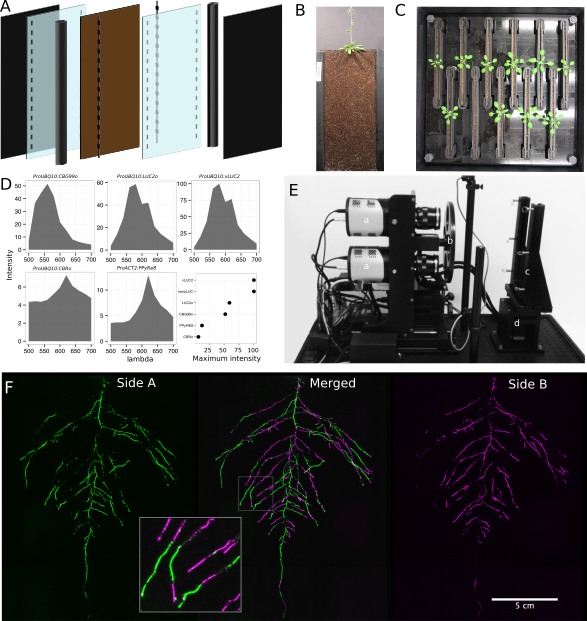
\includegraphics{/Users/rrellan/Dropbox/repos/GLO-Roots/figures/figure_pngs/figure_1.png}\\\textbf{Figure
1. GLO-Roots growth and imaging systems} A) 3D representation of the
different physical components of the rhizotron: plastic covers,
polycarbonate sheets, spacers and rubber U-channels. Blueprints are
provided in Supplementary material 1. In brown, soil layer. B) Thirty
five day-old plant in rhizotron with black covers removed. C) Top view
of holding box with eleven rhizotrons. D)In vivo emission spectra of
different luciferases used in this study. Transgenic homozygous lines
expressing the indicated transgenes were grown on agar media for 8 days.
Luciferin (300 µM) was sprayed on the seedlings and plates were kept in
the dark and then imaged for 2 s at wavelengths ranging from 500 to 700
nm. Five intensity values were taken from different parts of the roots
of different seedlings and averaged. Relative maximum intensity values
are indicated in the lower right graph. E) GLO 1 imaging system. The
system is composed by two back illuminated CCD cameras (a) cooled down
to -55 ºC. A filter wheel (b) allows for spectral separation of the
different luciferases. On the right, a rhizotron holder (c) is used to
position the rhizotrons in front of the cameras. A stepper motor (d)
rotates the rhizotron 180º to image both sides. F) A 21 DAS plant
expressing \emph{ProUBQ10:LUC2o} was imaged on each of two sides of the
rhizotron; luminescence signal is colorized in green or magenta to
indicate side. In the middle of the panel, a combined image of the two
sides is shown. The inset shows a magnified part of the root system. FW:
fresh weight, PR: Primary root.

\pagebreak

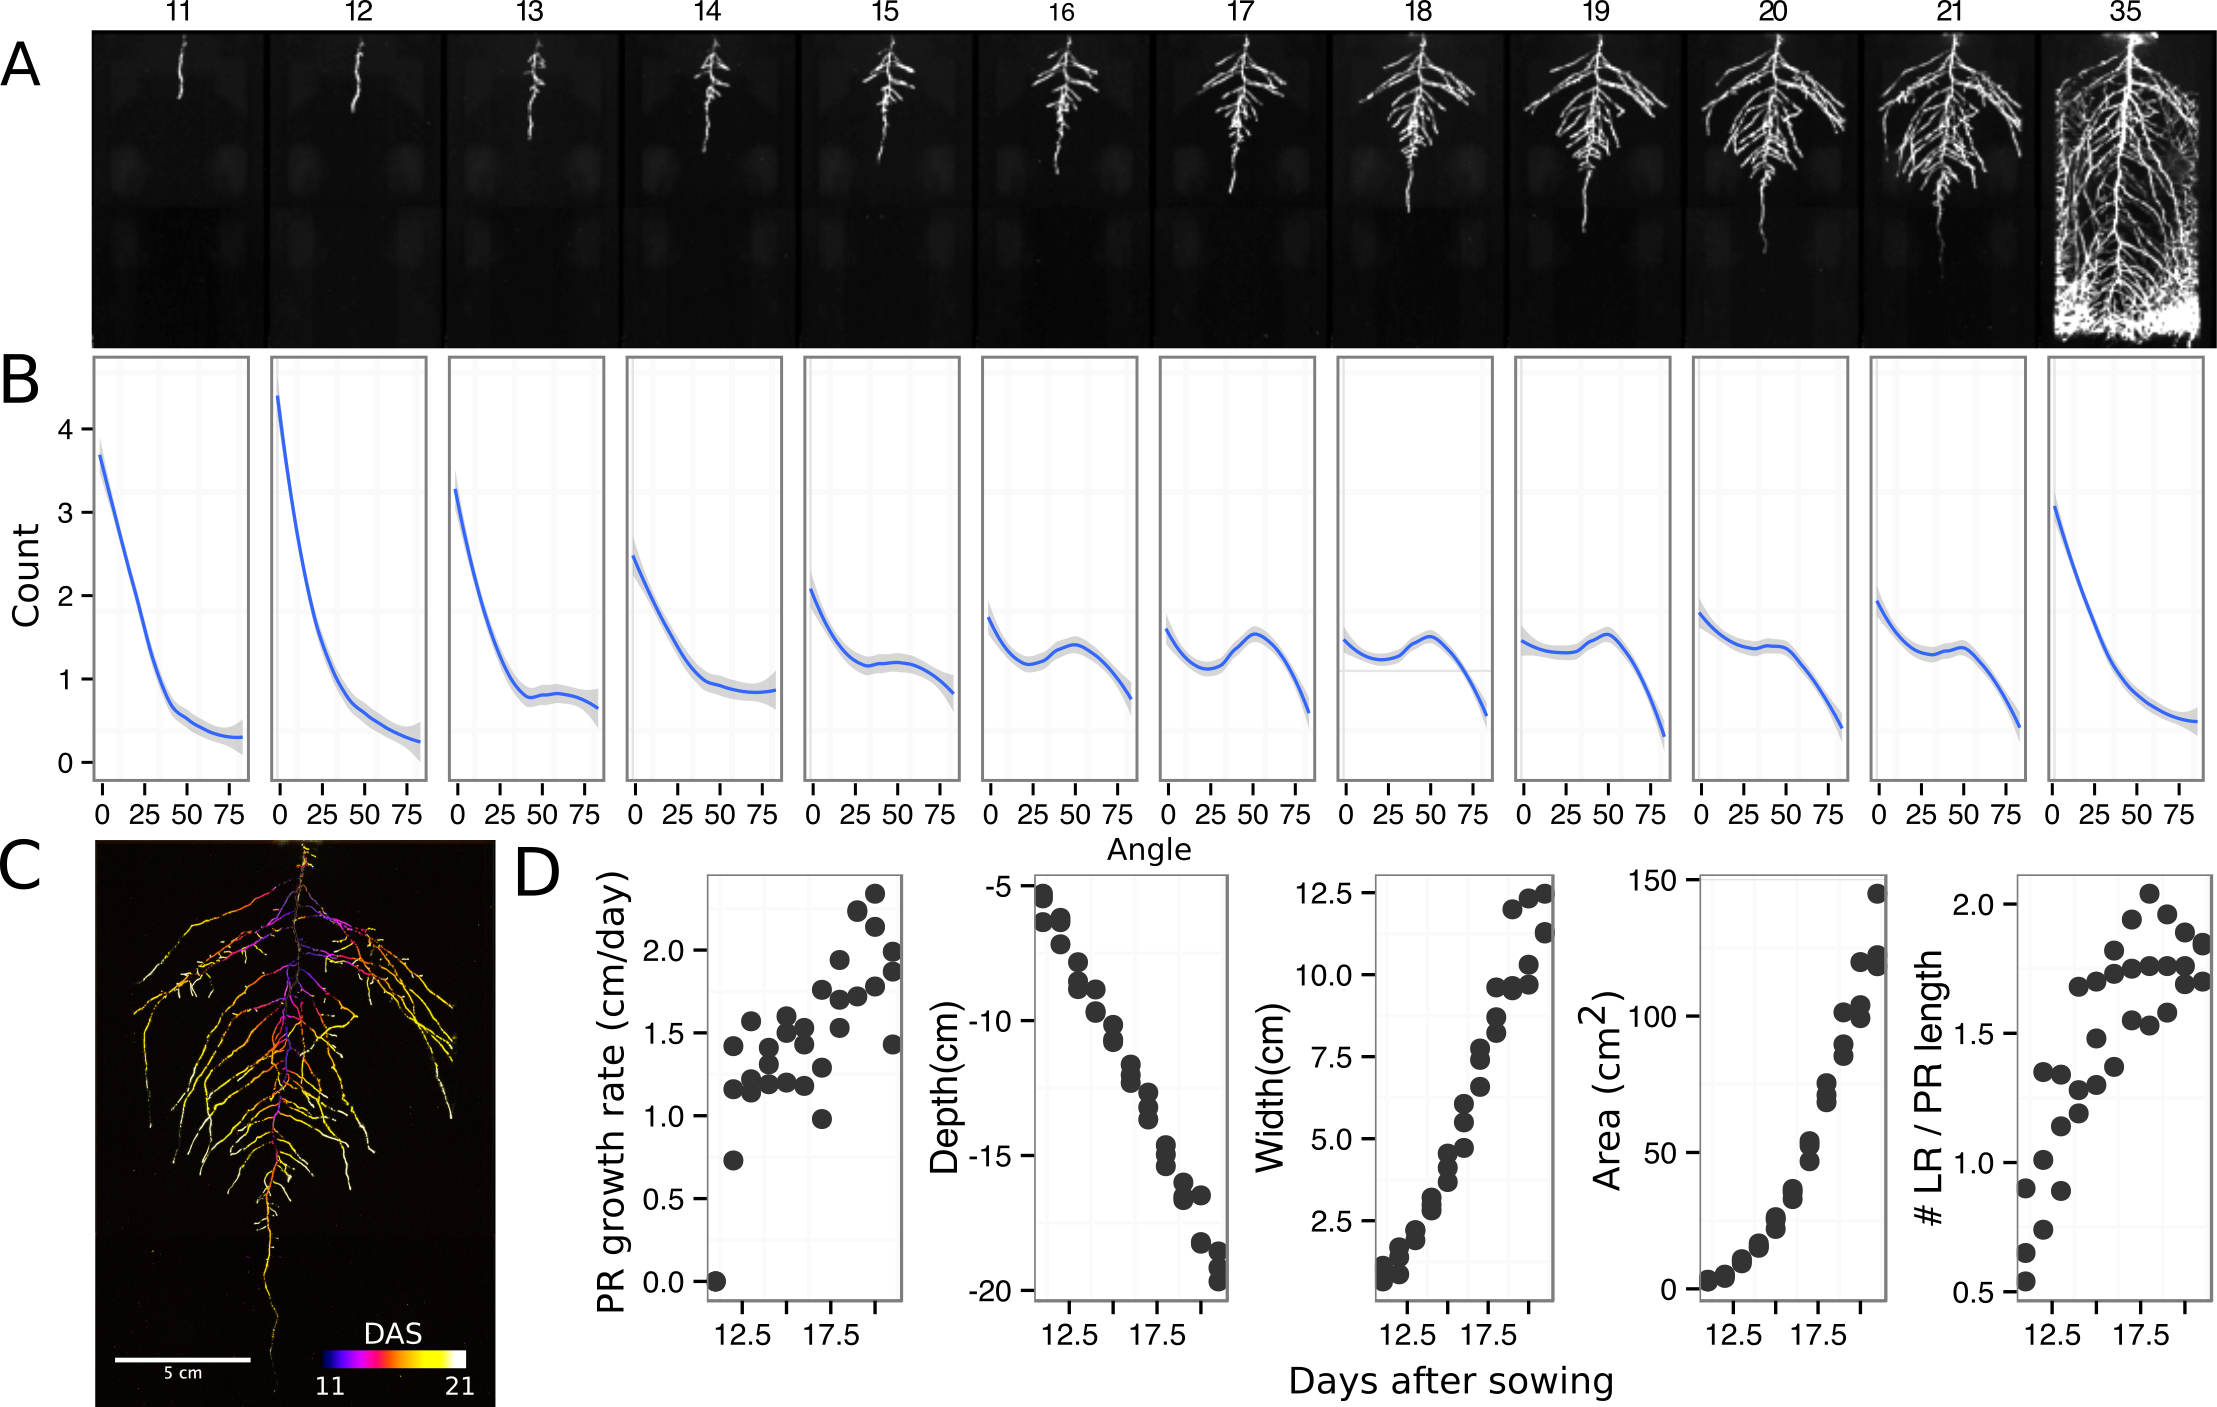
\includegraphics{/Users/rrellan/Dropbox/repos/GLO-Roots/figures/figure_pngs/figure_2.png}\\\textbf{Figure
2. Time-lapse imaging of root systems and quantification using GLO-RIA.}
A) Typical daily time-lapse image series from 11 to 35 DAS of a
\emph{ProUBQ10:LUC2o} Col-0 plant. B) Directionality of the root system
of plants in panel A calculated using the directionality plugin
implemented in GLO-RIA. C) Color coded projection of root growth using
the images in panel A. D) Primary root growth rate, depth, width, root
system area are automatically calculated from the convex hull, which is
semi-automatically determined with GLO-RIA. Lateral root number and
number of lateral roots divided by the primary root length were
quantified manually. A Local Polynomial Regression Fitting with 95\%
confidence interval (grey) was used to represent the directionality
distribution curve. (0º is the direction of the gravity vector).

\pagebreak

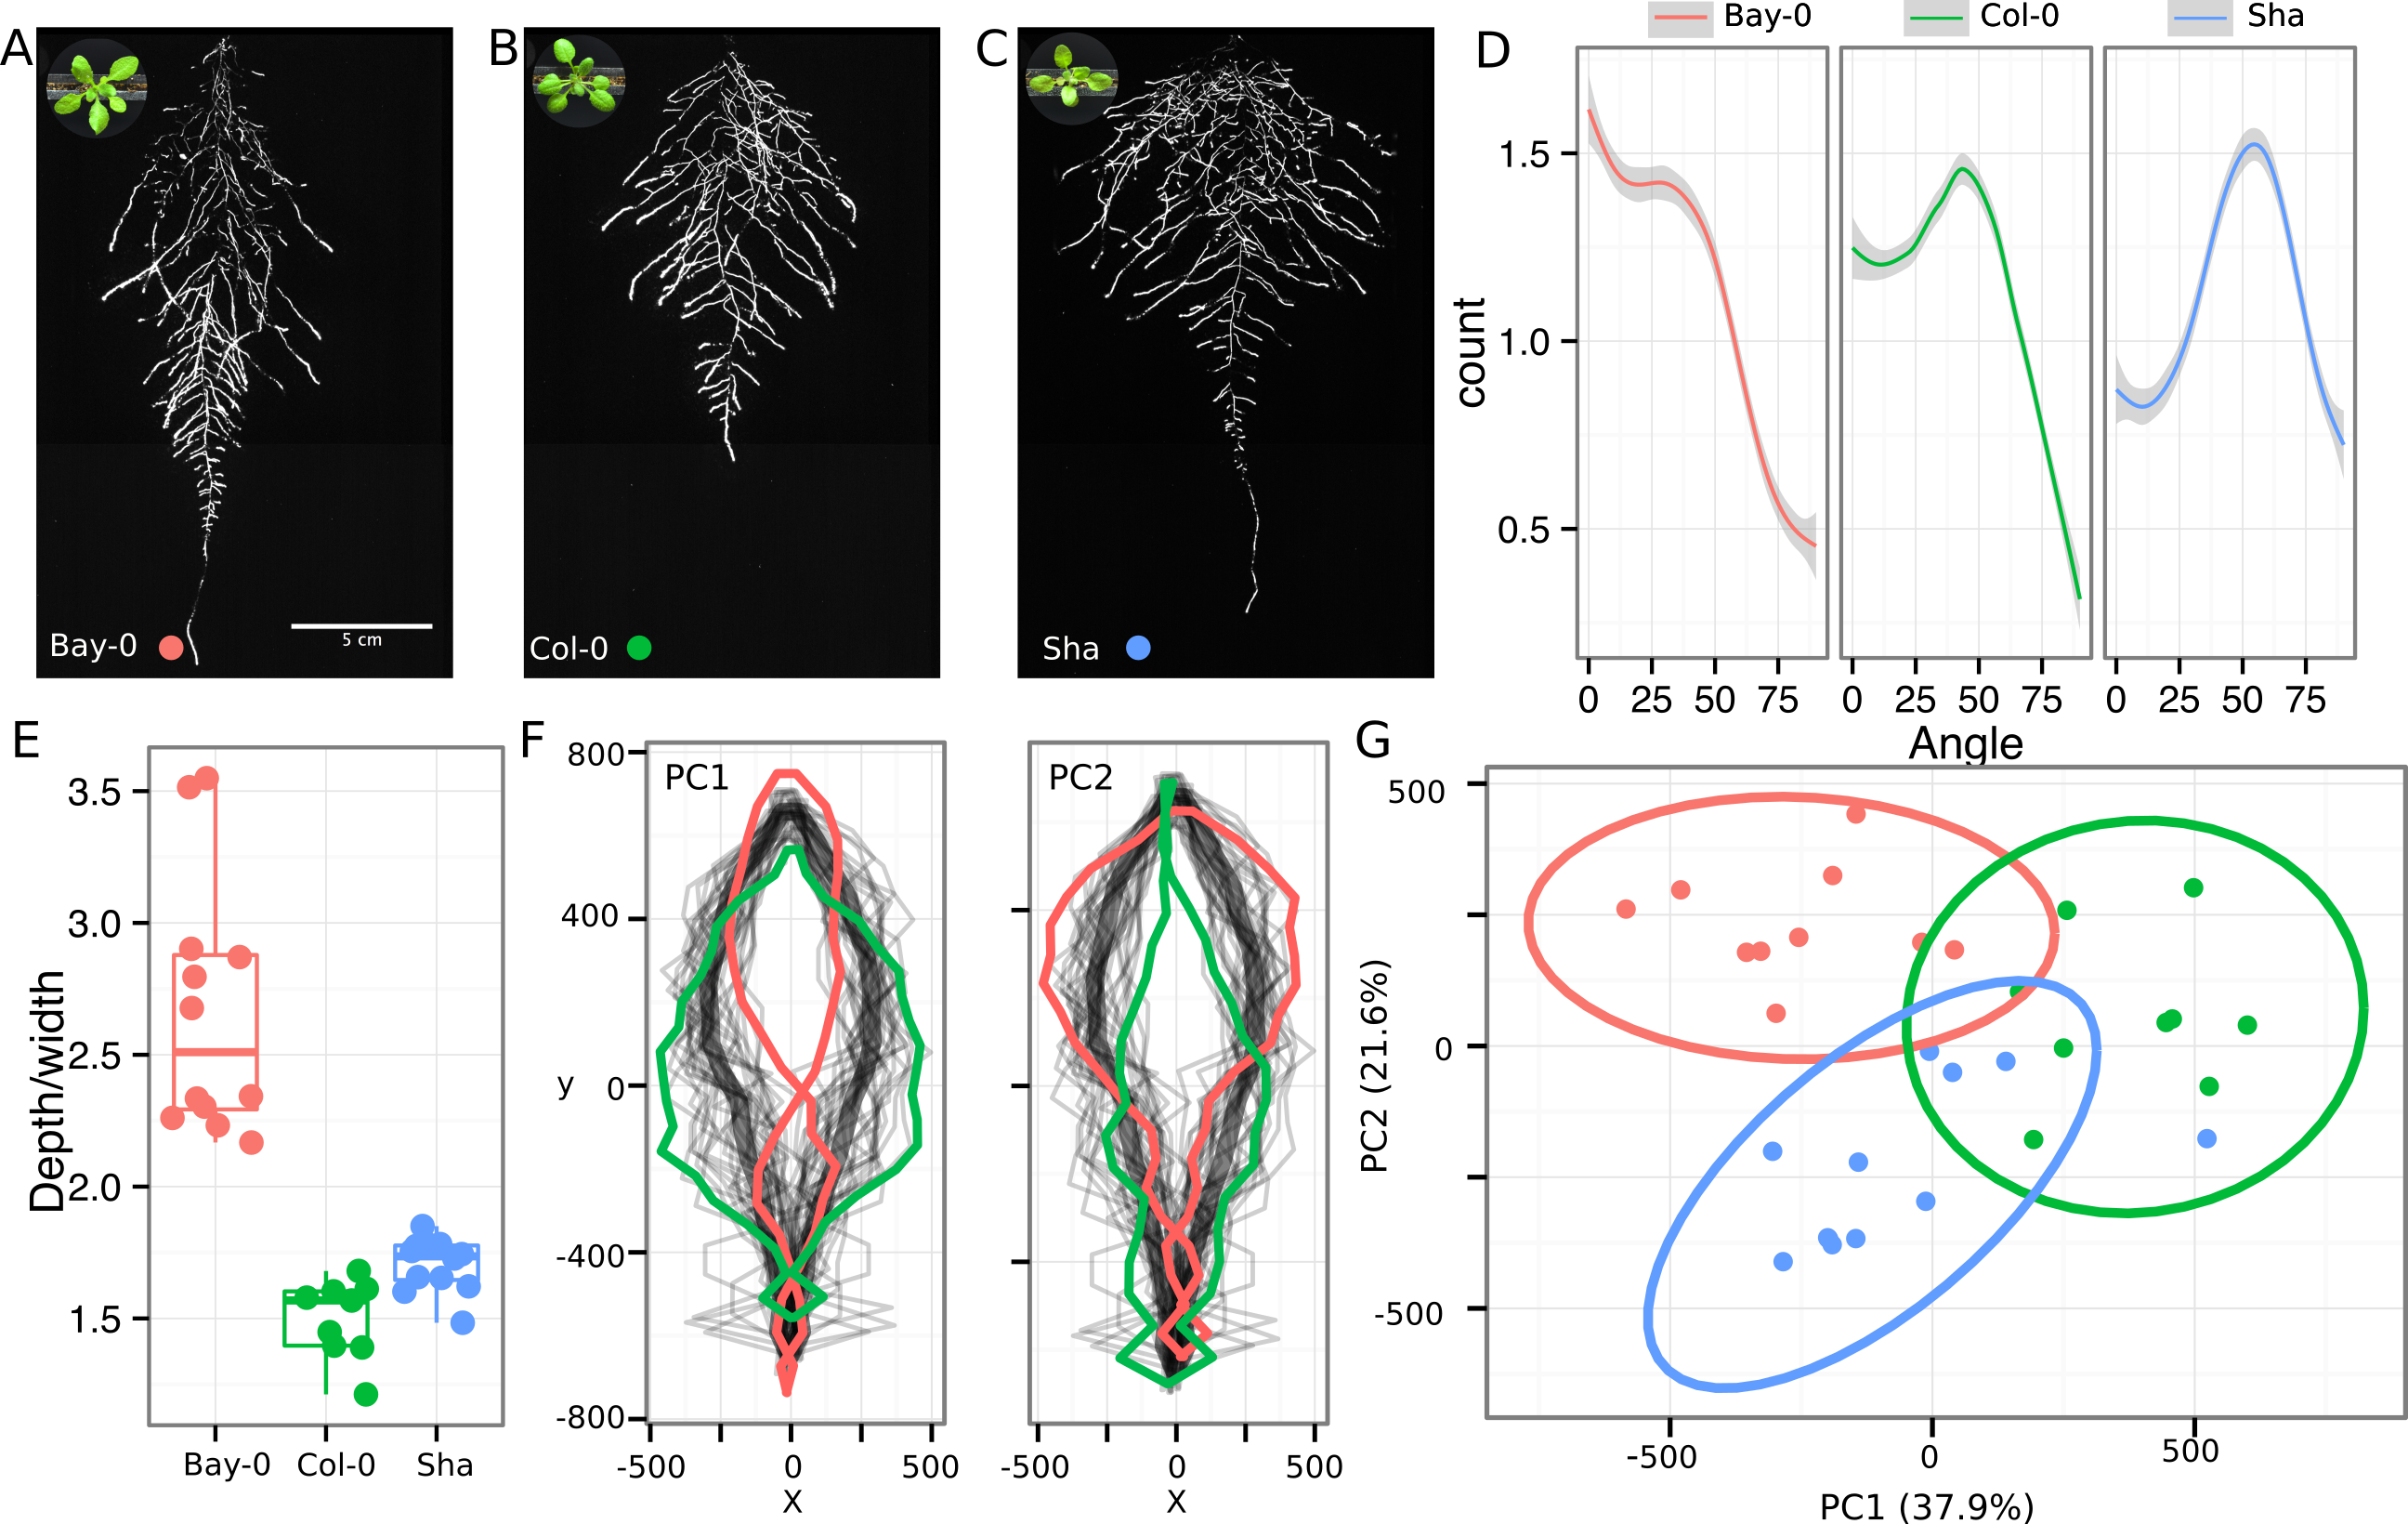
\includegraphics{/Users/rrellan/Dropbox/repos/GLO-Roots/figures/figure_pngs/figure_3.png}\\\textbf{Figure
3. Variation in root architecture between accessions of Arabidopsis.}
Representative root and shoot images of A) Bay-0, B) Col-0 and C) Sha
accessions transformed with \_ProUBQ10:LUC2o\_and imaged after 22 DAS.
D) Directionality of the root systems, E) depth/width ratio, F)
Pseudo-landmarks describing shape variation in root system architecture.
Eigenvalues derived from the analysis of 9-12 plants per accession is
shown. The first two Principal Components explaining 38\% (PC1) and 22\%
(PC2) of the shape variation are plotted. PC1 captures homogeneity of
root system width along the vertical axis and PC2 a combination of depth
and width in top parts of the root system. Red and green lines indicate
-3SD and +3SD (Standard Deviations), respectively G) PC separation of
the different ecotypes using the PCs described in (F). A Local
Polynomial Regression Fitting with 95\% confidence interval (grey) was
used to represent the directionality distribution curve. 0º is the
direction of the gravity vector. Wilcoxon test analysis with p
\textless{} 0.01 was used to test significant differences between the
different accession (n = 9-12 plants).

\pagebreak

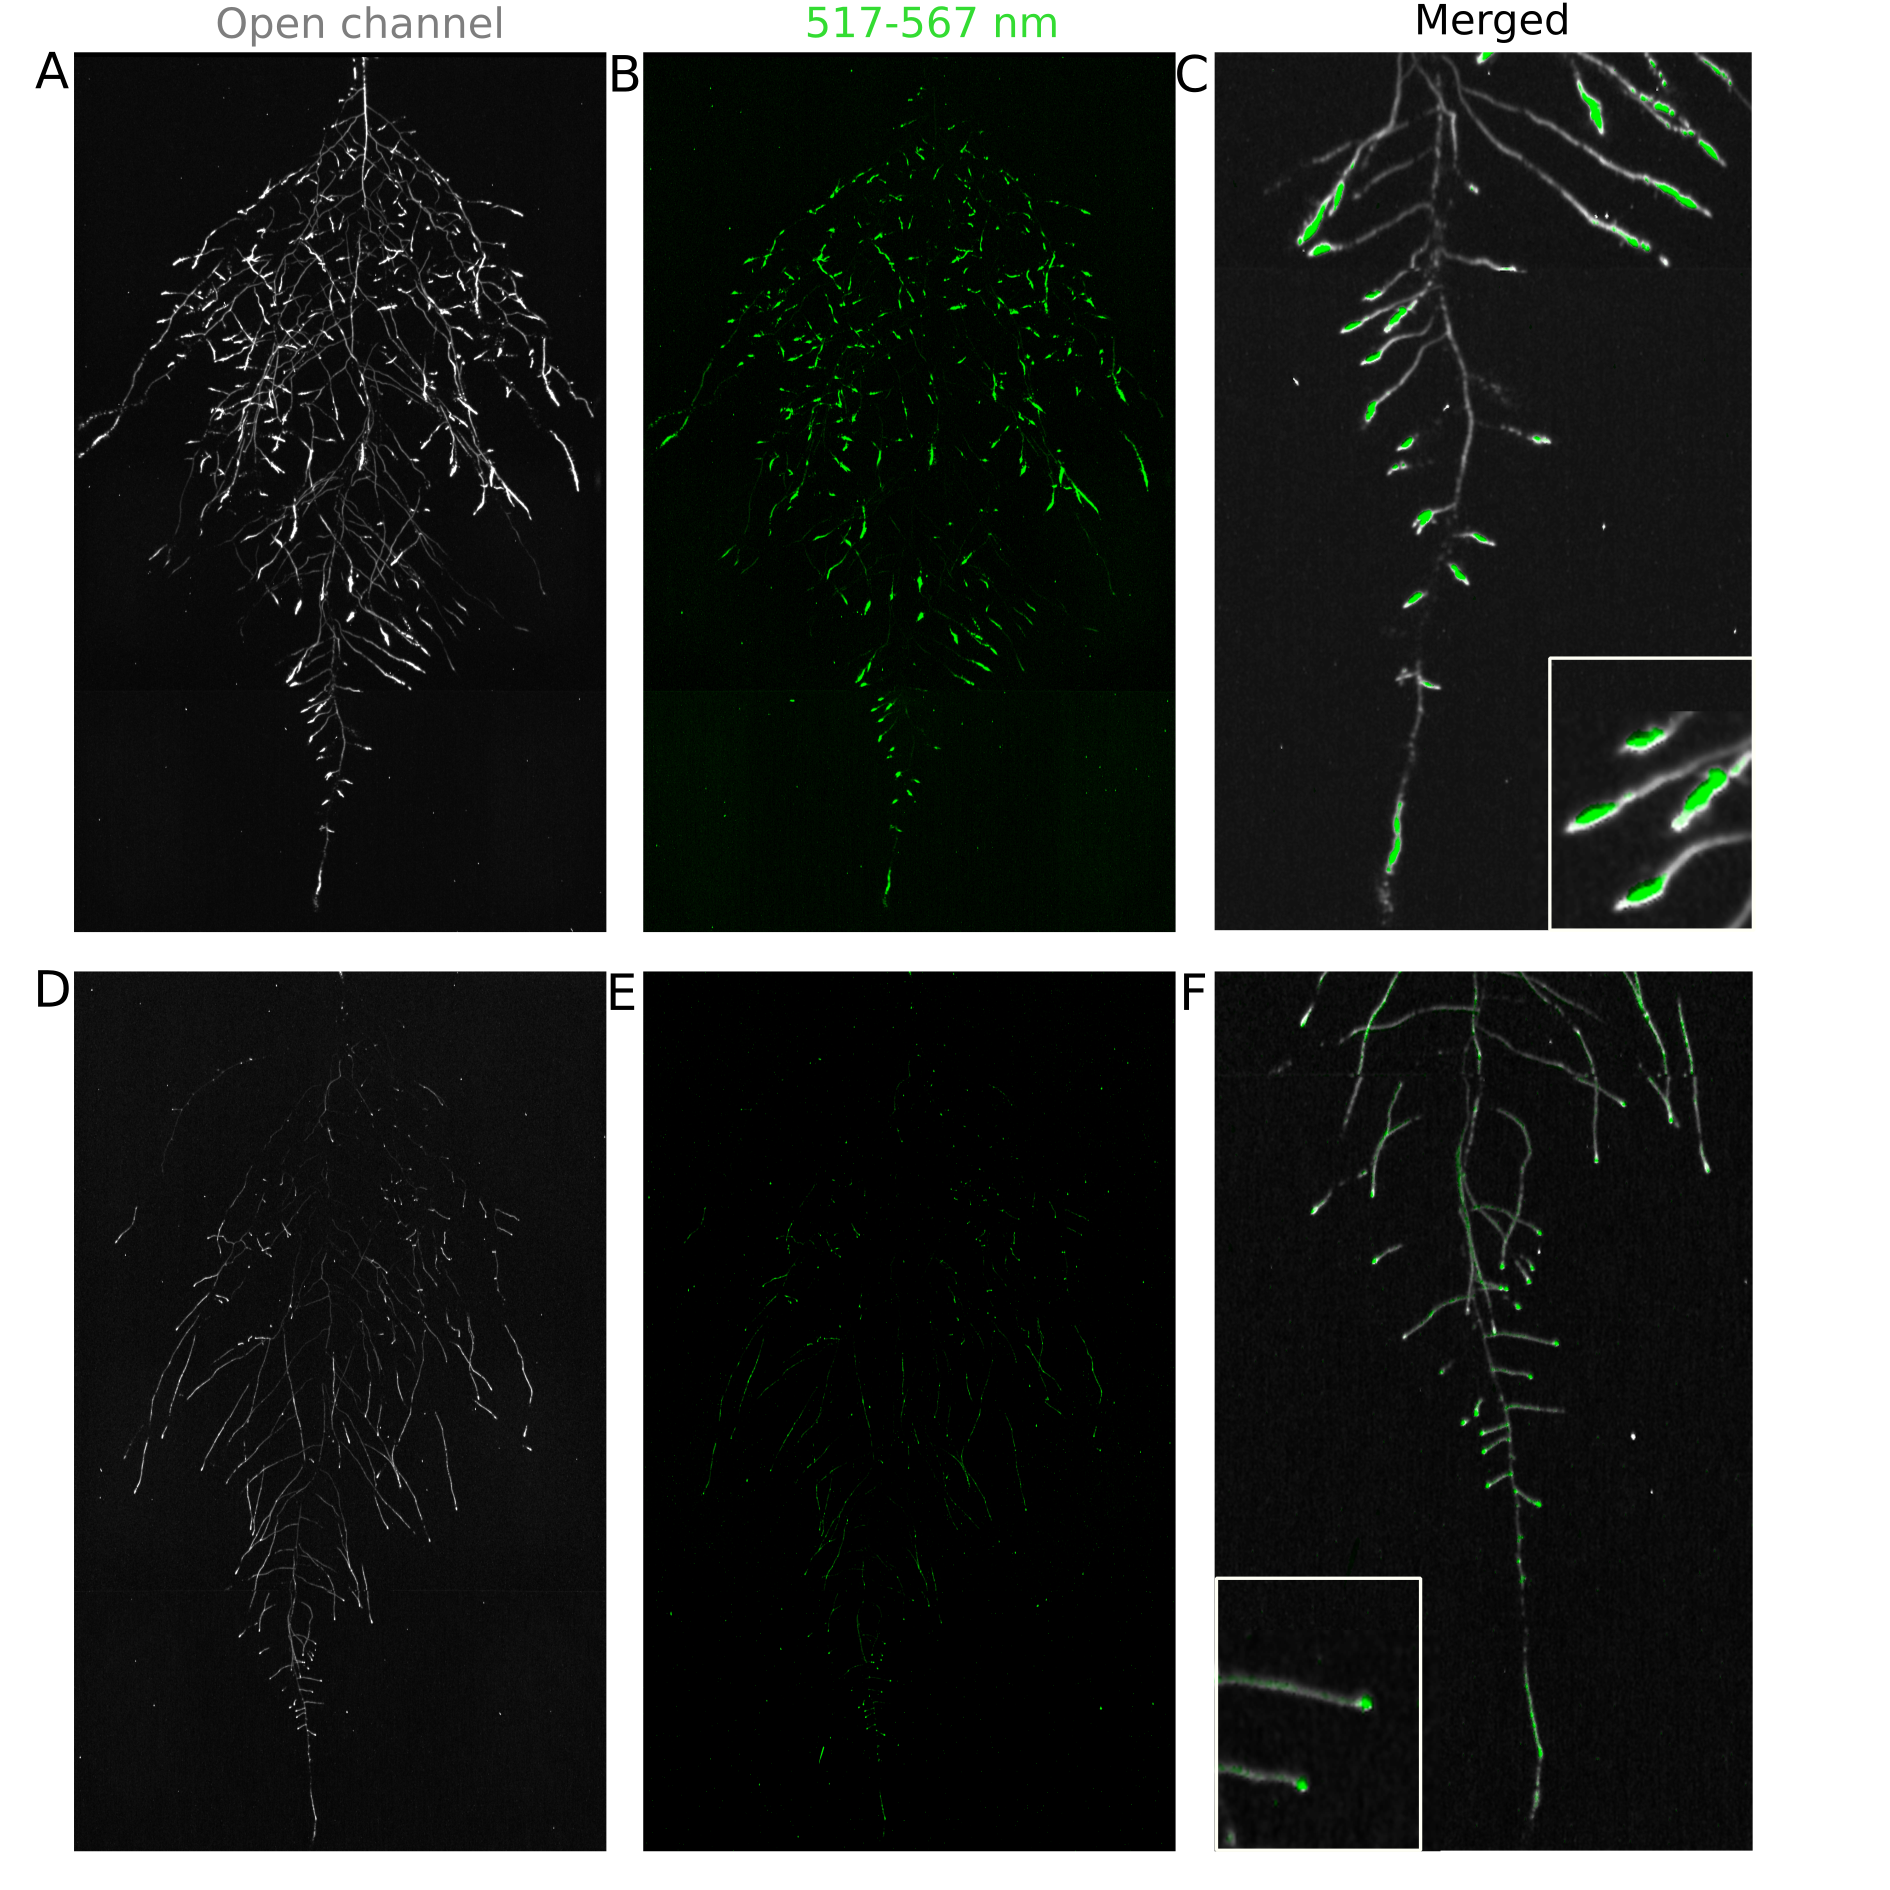
\includegraphics{/Users/rrellan/Dropbox/repos/GLO-Roots/figures/figure_pngs/figure_4.png}\\\textbf{Figure
4. Dual-color reporter visualization of structure and gene expression.}
Images of whole root systems (A, D) or magnified portion of roots (C, F)
at 22 DAS expressing \emph{ProDR5rev:LUC+} (green, A, B) or
\emph{ProZAT12:LUC} signal (green, D, E)with skeletonized representation
of roots generated using the \emph{ProACT2:PpyRE8o} reporter expression
(in grey).

\pagebreak

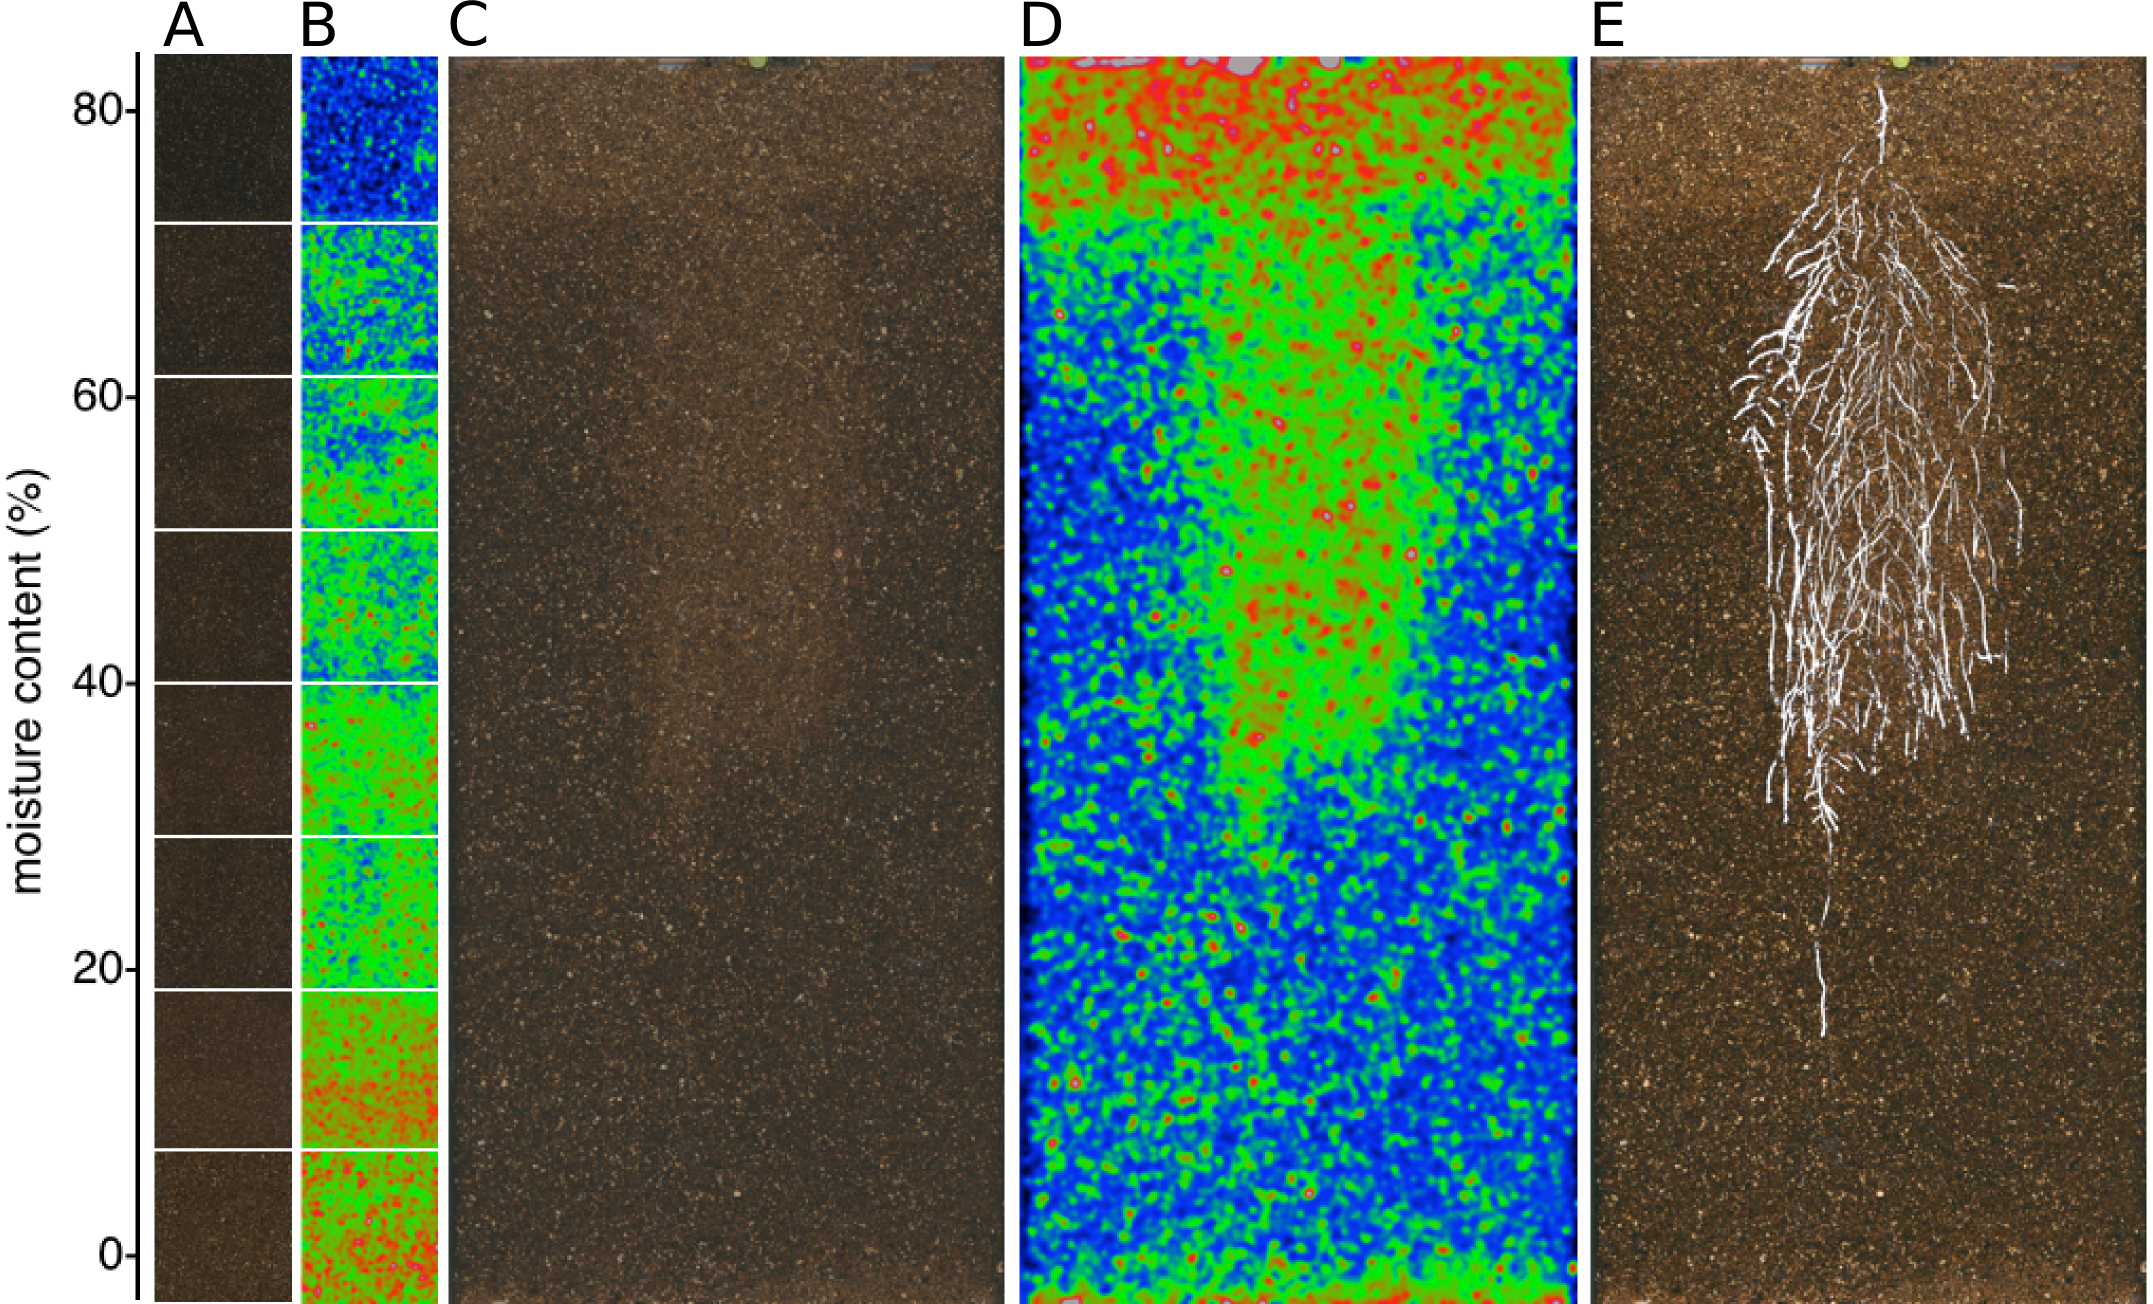
\includegraphics{/Users/rrellan/Dropbox/repos/GLO-Roots/figures/figure_pngs/figure_5.png}\\\textbf{Figure
5. Soil moisture and root architecture mapping in rhizotrons.} A)
Composite image showing regions of soil made from rhizotrons prepared
with different moisture levels. B) Differences in grey-scale intensity
values were enhanced using a 16-color Look Up Table (LUT). Brightfield
image of soil in rhizotron (C) and converted using 16-color LUT to
enhance visualization of distribution of moisture (D) . E) Root system
of a Bay-0 22 DAS and subjected to water deprivation since 13 DAS. Root
system visualized using luminescence and overlaid on brightfield image
of soil in (C).

\pagebreak

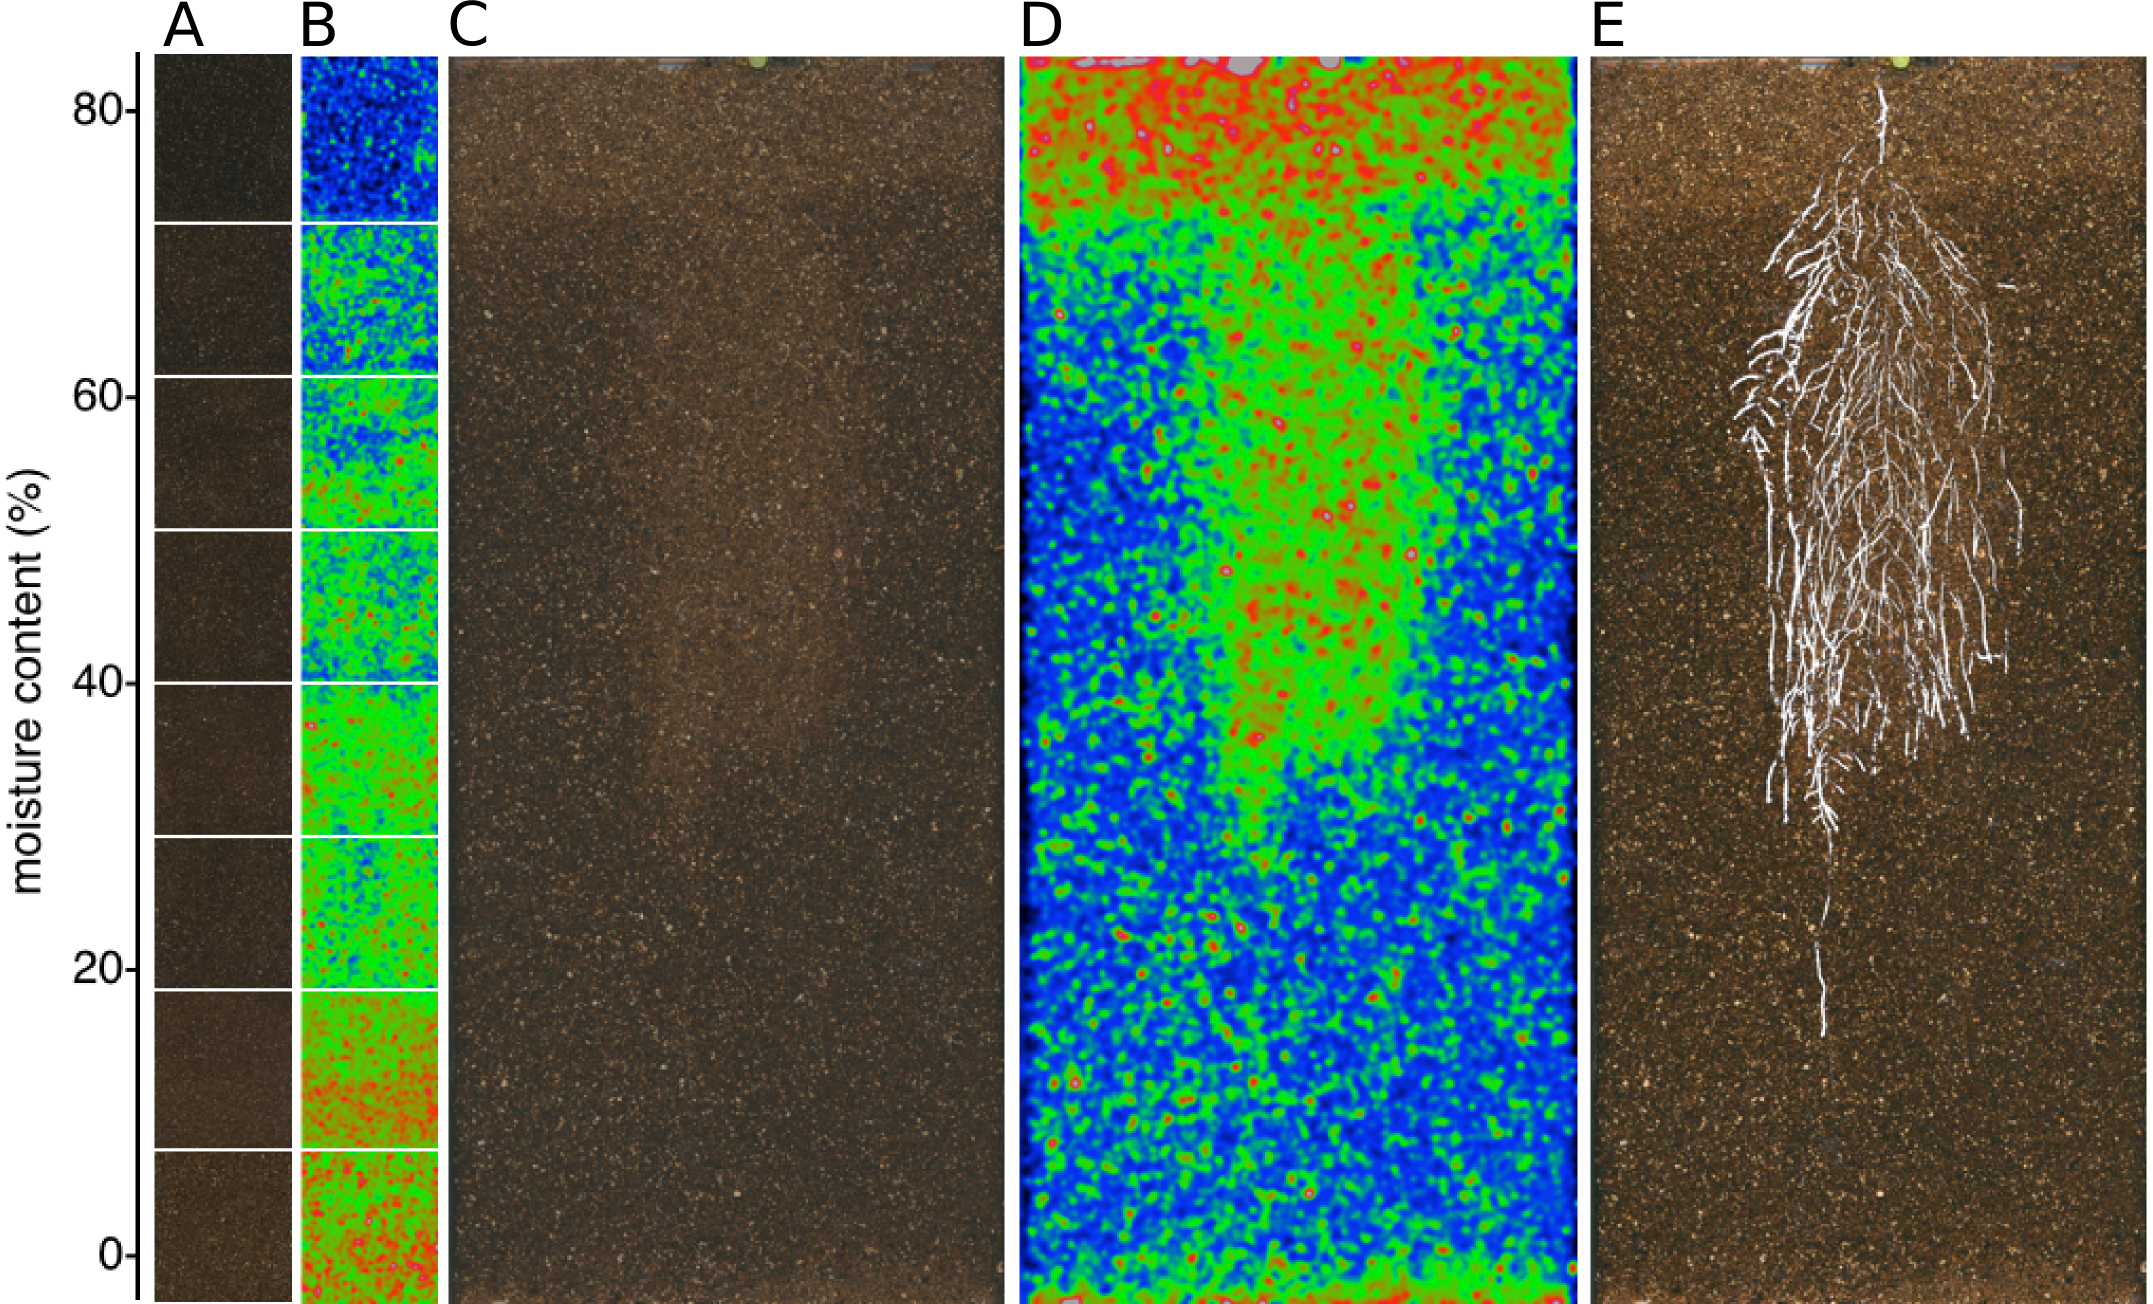
\includegraphics{/Users/rrellan/Dropbox/repos/GLO-Roots/figures/figure_pngs/figure_6.png}\\\textbf{Figure
6. Study of effect of water deficit on root system architecture.} A-D)
Root systems 22 DAS and exposed to water deficit 13 DAS onwards. Sample
images of well watered (left panels) and water deficit (right panels)
root systems treated from 13 DAS and directionality (line graphs to left
of images) for (A) Col-0 (B) Bay-0 (C) \emph{miz1} mutant and (D)
\emph{tir1-1} . E) Root system of a 22 DAS plant exposed to water
deprivation from 9 DAS onwards with magnified view of lateral root
primordia (F). G) The same root as in (E) 24 hours after rewatering and
magnified view of lateral root primordia (H). Kolmogorov-Smirnov test at
p \textless{} 0.001 was used to compare directionality distributions
between the different treatments and genotypes. A Local Polynomial
Regression Fitting with 95\% confidence interval (grey) was used to
represent the directionality distribution curve. 0º is the direction of
the gravity vector.

\pagebreak

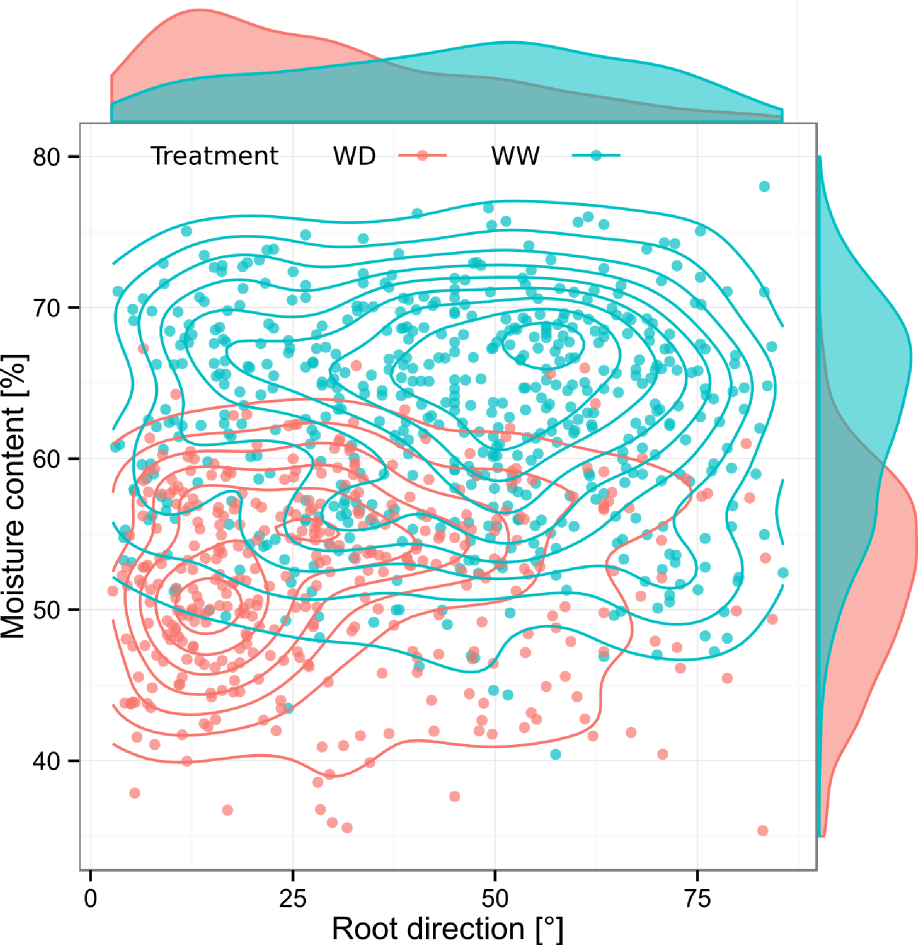
\includegraphics{/Users/rrellan/Dropbox/repos/GLO-Roots/figures/figure_pngs/figure_7.png}\\\textbf{Figure
7. Relationship between local soil moisture content and root growth
direction.} Data quantified from the time lapse series shown in
\href{https://www.dropbox.com/s/x24x1uhvc8x0ou9/Video_3.avi?dl=0}{Video
2}. Density plots shown at periphery of graph for root direction
(x-axis) and soil moisture (y-axis). 0º is the direction of the gravity
vector. Data represents 2535 root tips measured in a series encompassing
10 time points.

\pagebreak

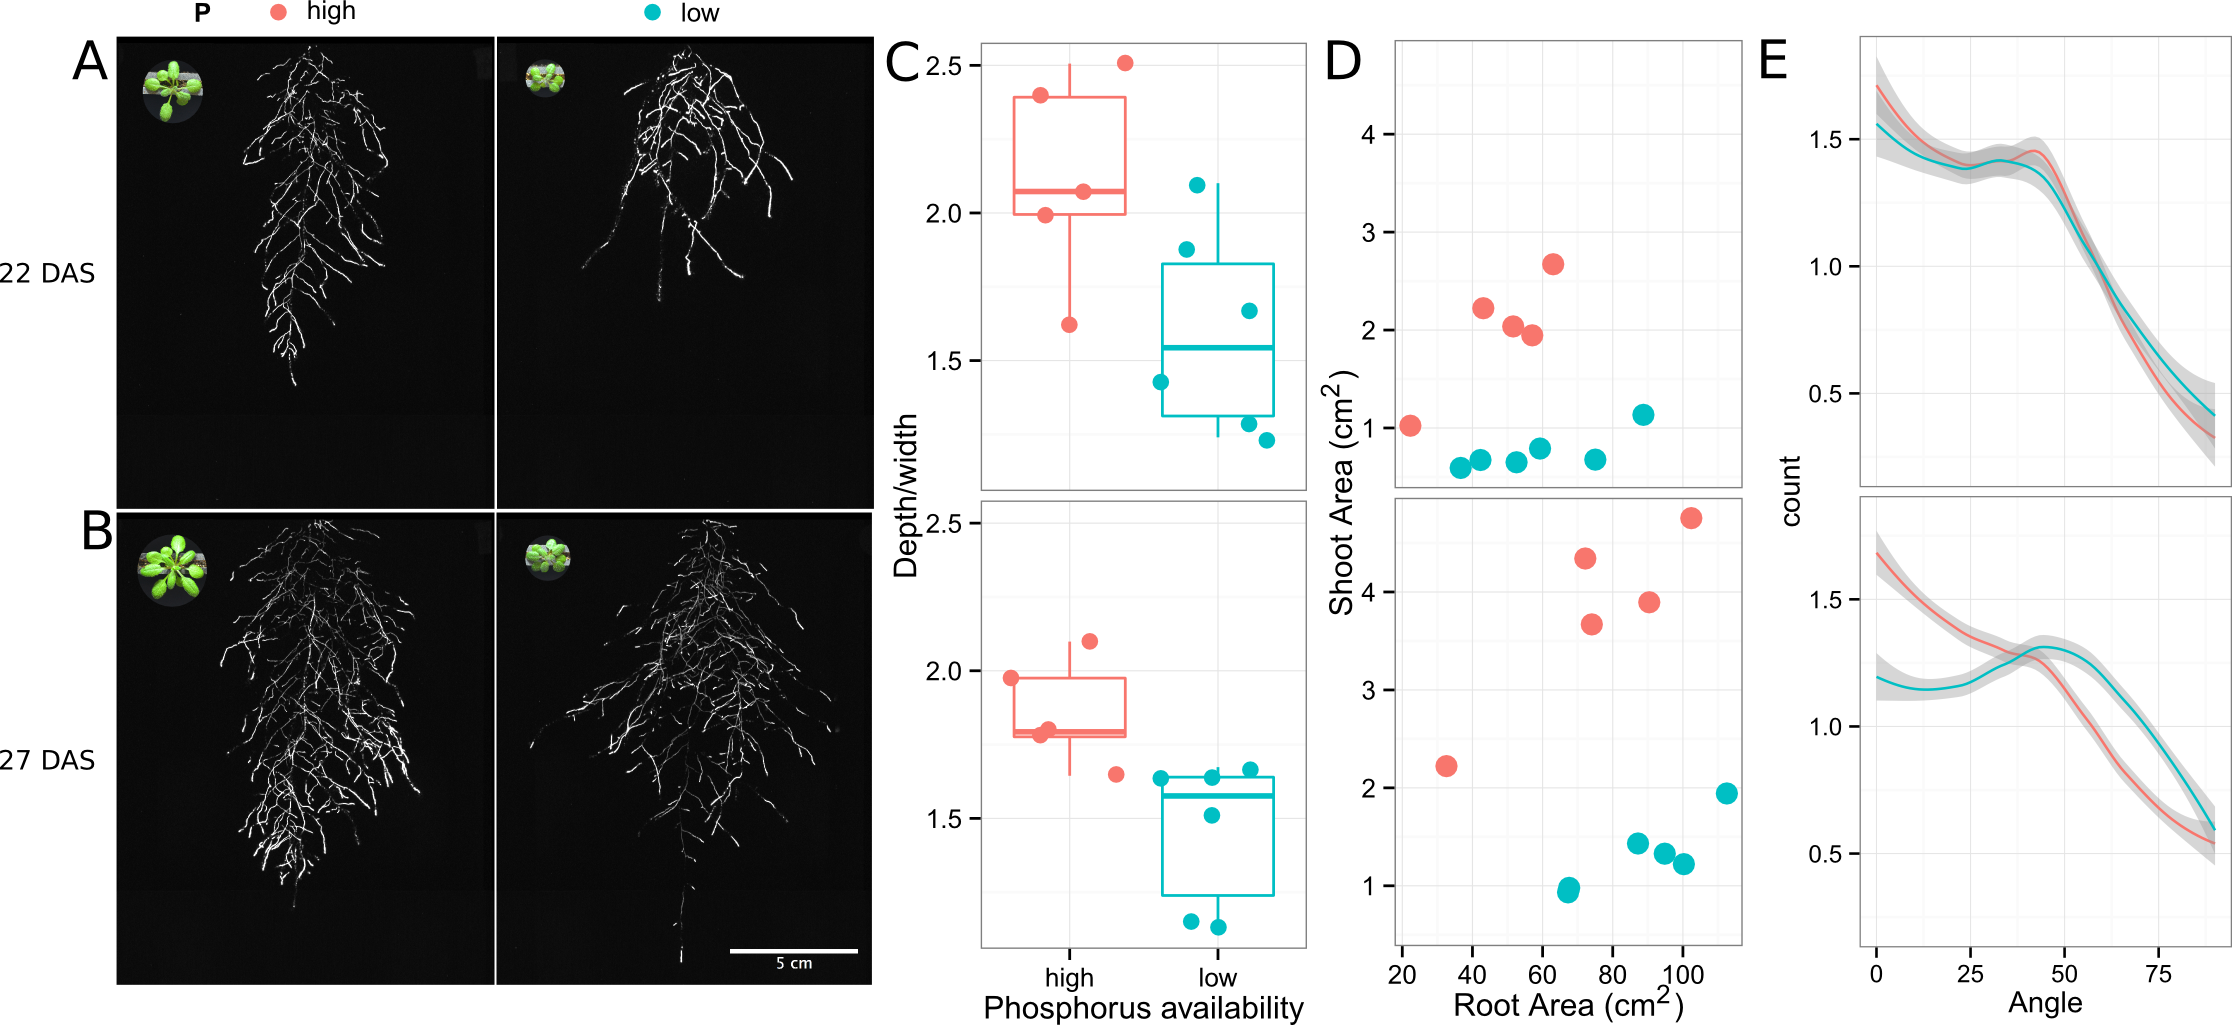
\includegraphics{/Users/rrellan/Dropbox/repos/GLO-Roots/figures/figure_pngs/figure_8.png}\\\textbf{Figure
8}: Roots of \emph{Brachypodium distachyon} transformed with
\emph{ProZmUB1:LUC2o} and imaged at 15 (A) and 24 (B) DAS grown in
control conditions. C) Open channel of 17 DAS tomato plant transformed
with \emph{ProeDR5rev:LUC2o} and \emph{Pro35S:PPyRE8o} D) Green channel
showing only \emph{ProeDR5rev:LUC2o} E) Amplification of the open and
green channel showing increased expression of \emph{ProeDR5rev:LUC2o}
reporter in early-stage lateral roots.

\pagebreak

\subsection{Videos}\label{videos}

\href{https://www.dropbox.com/s/sxjc04o0yj2faif/Video_1.avi?dl=0}{\textbf{Video
1}} Time lapse from 11 to 21 DAS of a Col-0 plant expressing
ProUBQ10:LUC2o grown in control conditions

\href{https://www.dropbox.com/s/x24x1uhvc8x0ou9/Video_3.avi?dl=0}{\textbf{Video
2}} Time lapse from 16 to 24 DAS of Col-0 plants expressing
\emph{ProUBQ10:LUC2o} growing in water deficient (left) and control
(right) conditions. Plants were sown under control conditions and water
deficit treatment started 11 DAS. Images were taked every day.

\pagebreak

\subsection{Supplementary Material}\label{supplementary-material}

\subsubsection{Supplementary figures}\label{supplementary-figures}

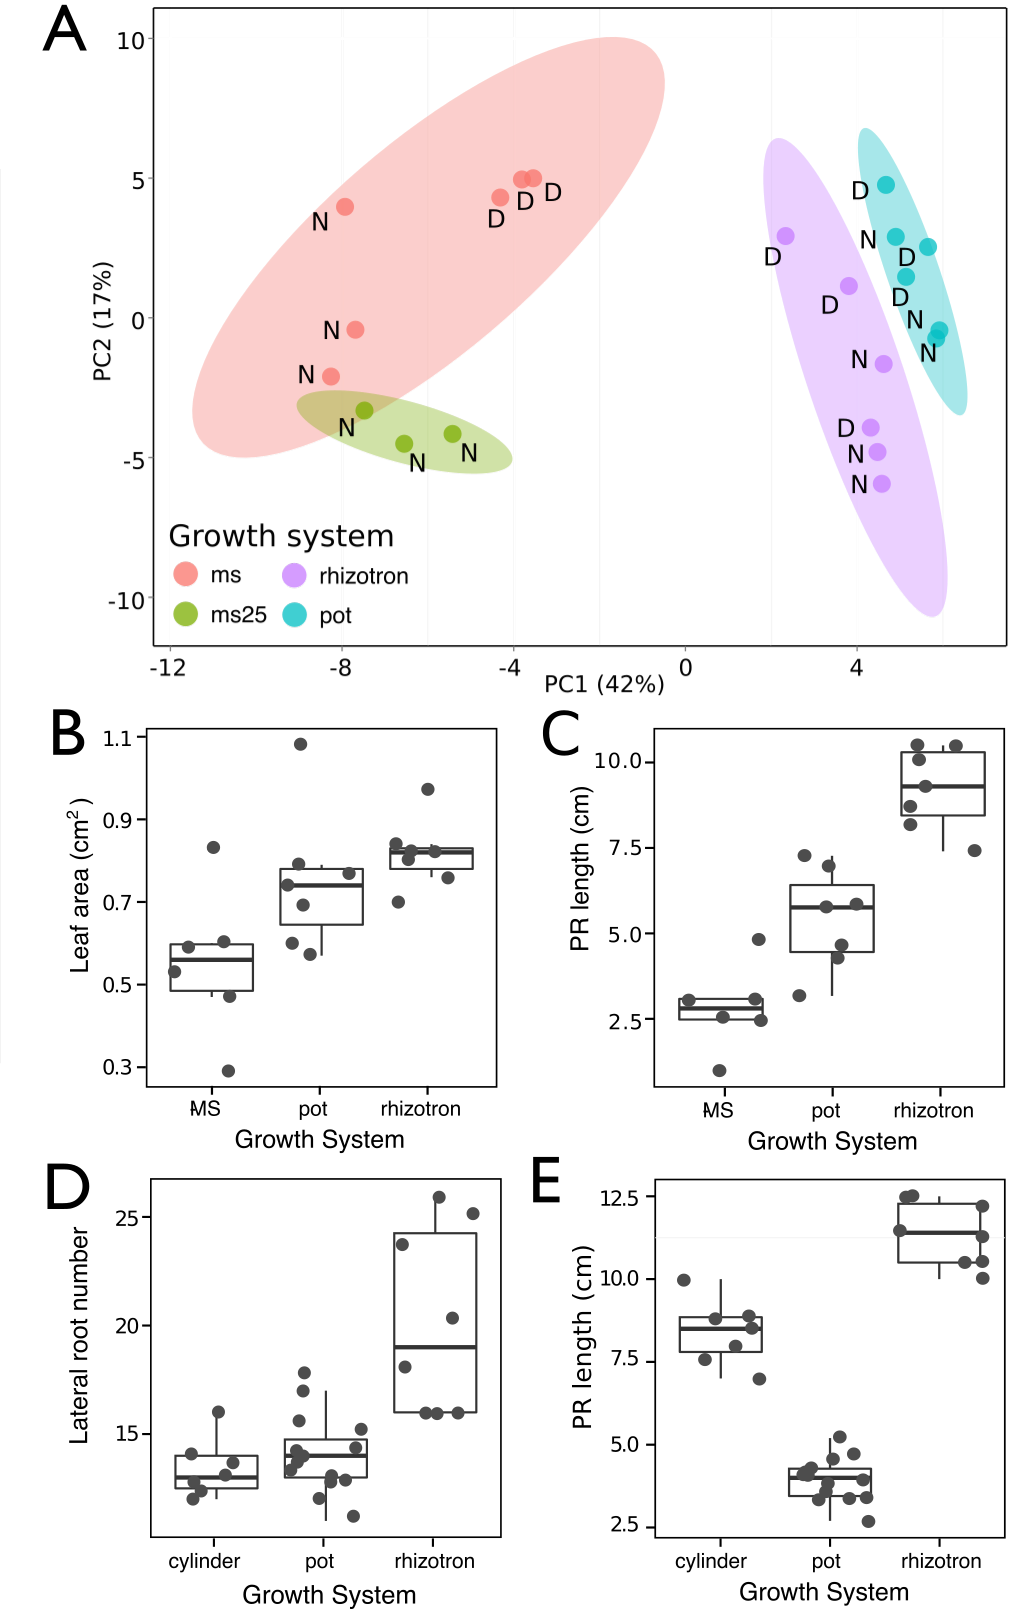
\includegraphics{/Users/rrellan/Dropbox/repos/GLO-Roots/figures/Supplements/Figure_1_figure_supplement_1.png}\\\textbf{Figure
1-figure supplement 1. Effect of different growth systems on plant
biology.} A) Principal Components Analysis (PCA) score plot of a set of
76 genes analyzed by qPCR from root samples of plants grown in MS
plates, pots, and rhizotrons. After 15 DAS three plants were collected
at the end of the day (D) and three were collected at the end of the
night (N). (ms = plant grown in full ms and 1\% sucrose, ms25 = plants
grown in 25\% of full ms) B) Lateral root number and G) primary root
length of 18 DAS plants grown in 30 cm tall cylinders, pots and
rhizotrons, all with a volume of 100 cm\textsuperscript{3} (n = 6-12
plants). D) Leaf area and E) primary root length of plants of the same
age (15 DAS) as the ones used for the qPCR experiment (n= 6-7). ANOVA
analysis with p \textless{} 0.01 was used to test significant
differences between the different parameters.

\pagebreak

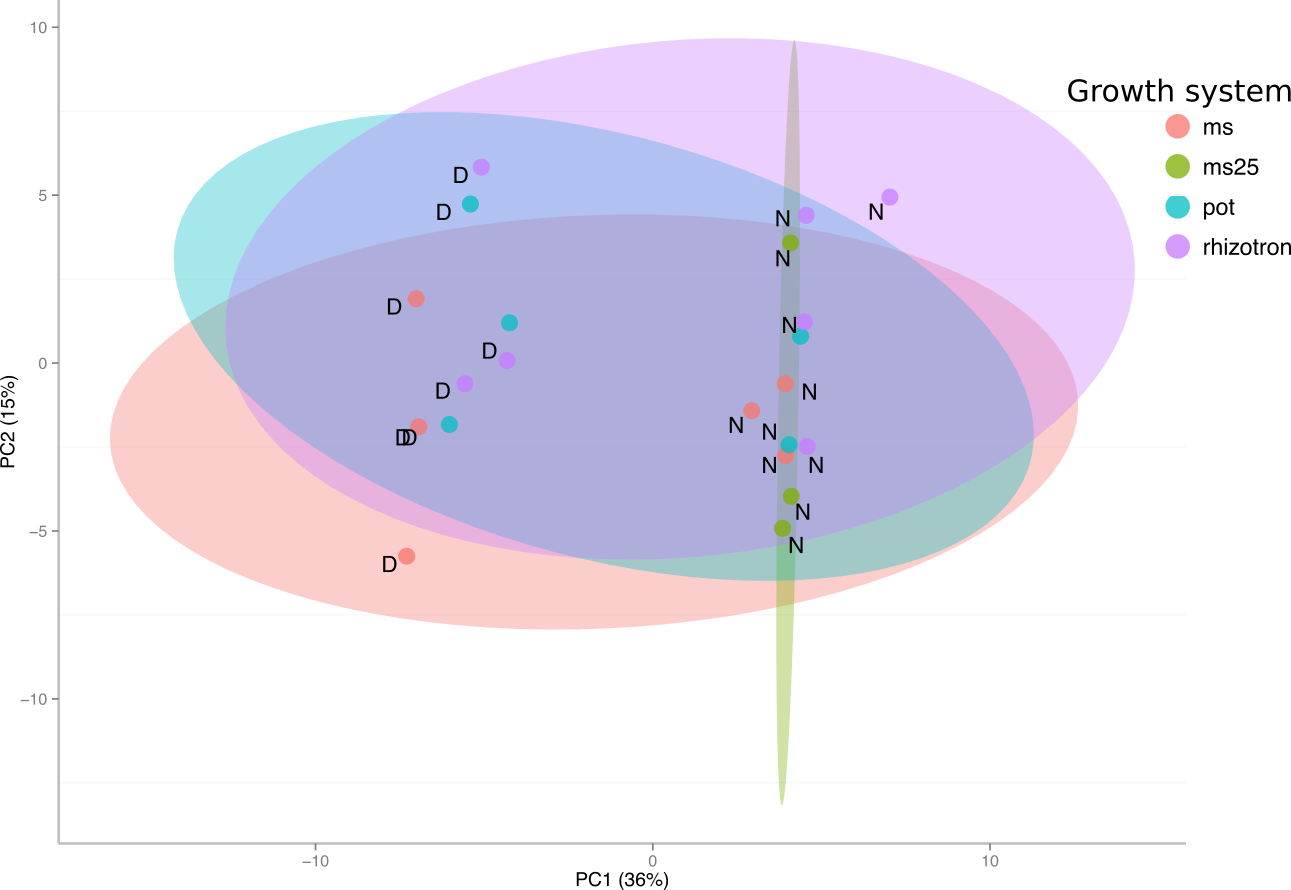
\includegraphics{/Users/rrellan/Dropbox/repos/GLO-Roots/figures/Supplements/Figure_1_figure_supplement_2.png}\\**Figure
1-figure supplement 2. PCA plot of shoots of the same samples analyzed
in Figure 1. See Figure 1 for more details regarding experimental
conditions used.

\pagebreak

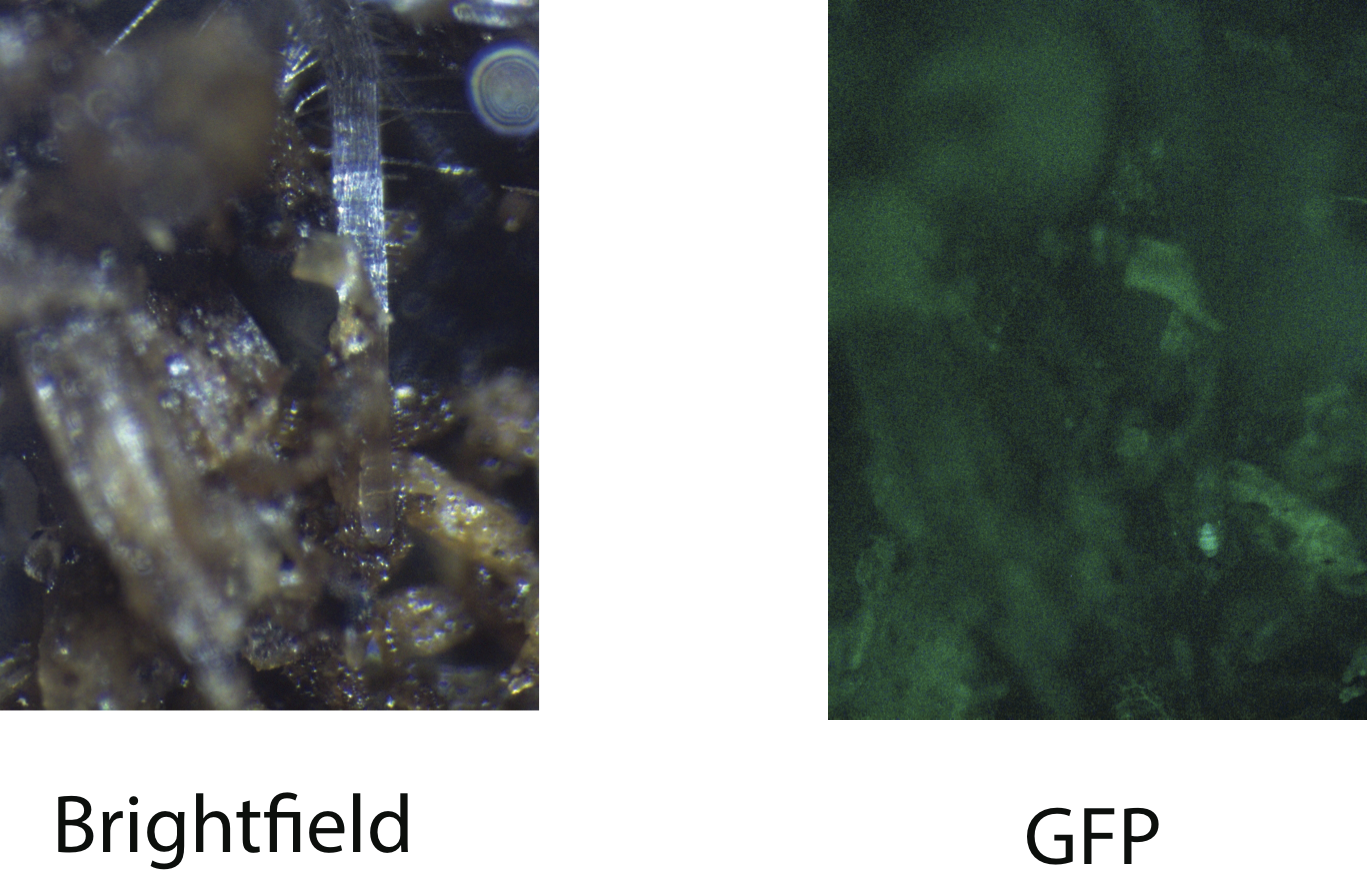
\includegraphics{/Users/rrellan/Dropbox/repos/GLO-Roots/figures/Supplements/Figure_1_figure_supplement_3.png}\\\textbf{Figure
1-figure supplement 3} Image of an Arabidopsis root in soil imaged with
white light (brightfield) or epifluorescence.

\pagebreak

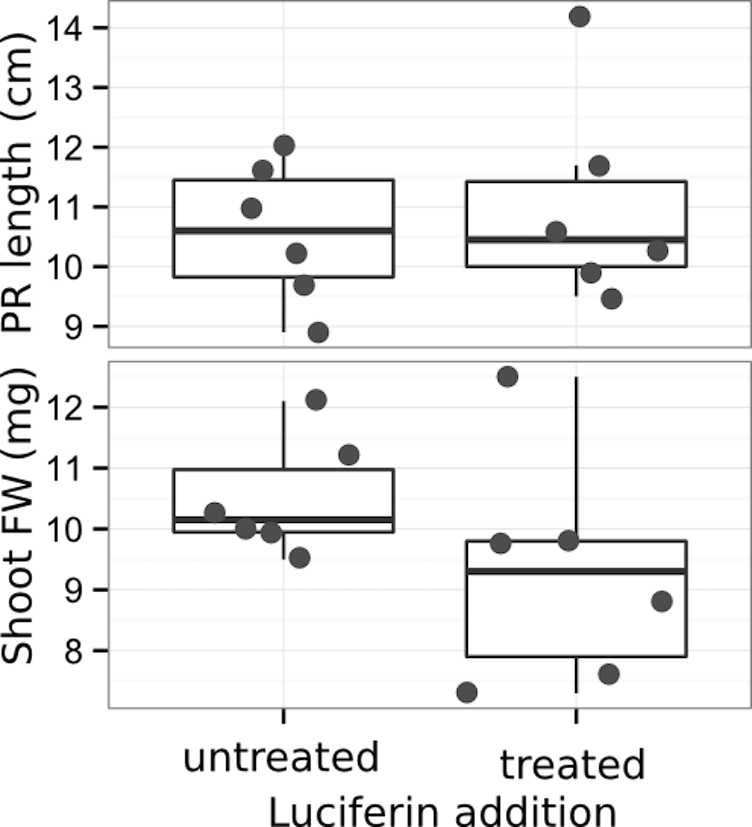
\includegraphics{/Users/rrellan/Dropbox/repos/GLO-Roots/figures/Supplements/Figure_1_figure_supplement_4.png}\\\textbf{Figure
1-figure supplement 4} Effect of luciferin addition on primary root
length and shoot size of 14 DAS seedlings that were either continuously
exposed to 300 µM luciferin from 9 DAS after sowing or not.

\pagebreak

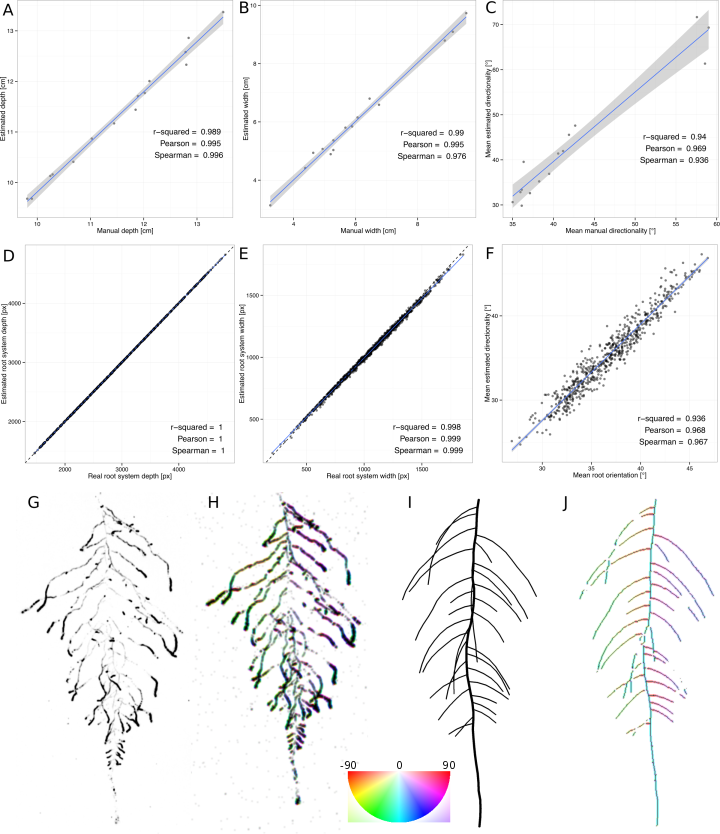
\includegraphics{/Users/rrellan/Dropbox/repos/GLO-Roots/figures/Supplements/Figure_1_figure_supplement_5.png}\\\textbf{Figure
1-figure supplement 5} GLO-RIA validation. Validation was carried out
using two approaches. We first used manually quantified root system
depth (A) width (B) and average lateral root angles (C) in a set of 15
root systems corresponding to different Arabidopsis accesions. We then
generated 1240 contrasting root systems using ArchiSimple as a ground
truth to validate root system depth (D) width (E) and directionality
(F). Example of a real (G) and ArchiSimple generated (H) root systems
and corresponding GLO-RIA color-coded directionality (I, J).

\pagebreak

\textbf{Figure 1-figure supplement data 1}: Two way ANOVA P-values
comparing plants grown in MS media vs.~plants grown in soil (pots or
rhizotrons) and plants collected at day or night. We used p-value
\textless{} 0.00065 threshold based on Bonferoni adjustment for multiple
testing.

\pagebreak

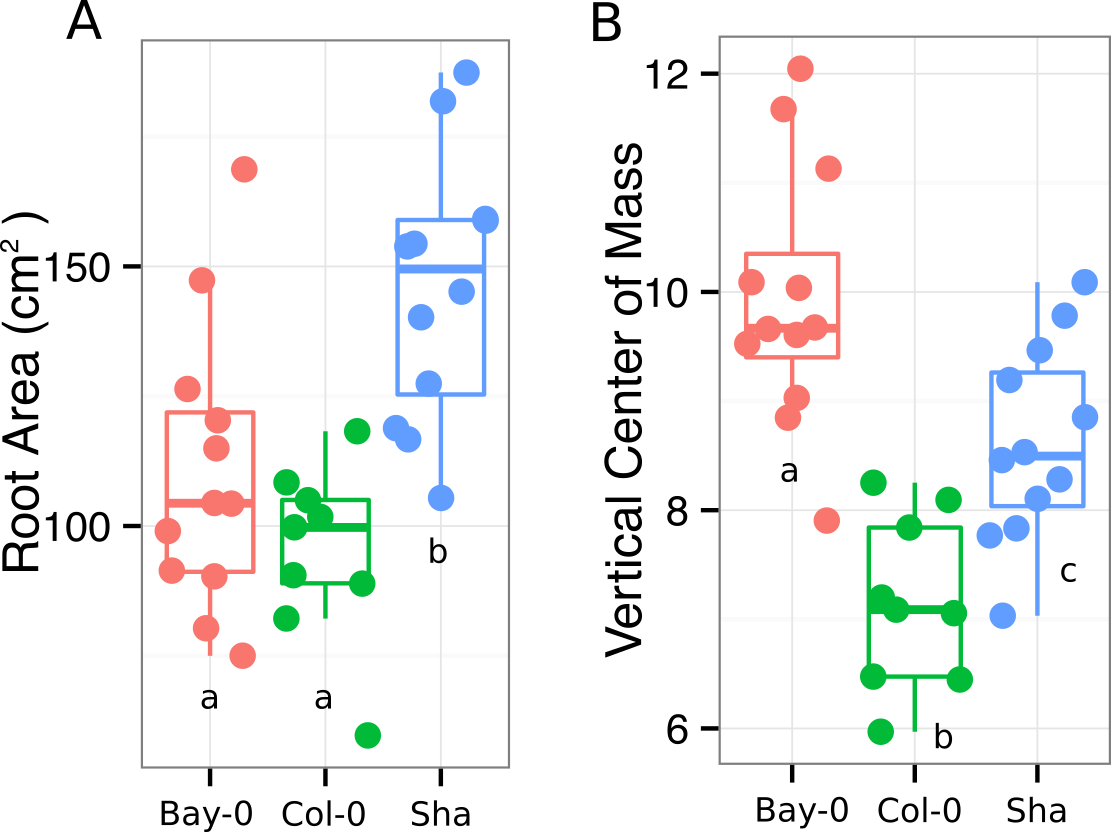
\includegraphics{/Users/rrellan/Dropbox/repos/GLO-Roots/figures/Supplements/Figure_3_figure_supplement_1.png}\\\textbf{Figure
3-figure supplement 1} A) root area, B) vertical center of mass of
Bay-0, Col-0 and Sha accessions.

\pagebreak

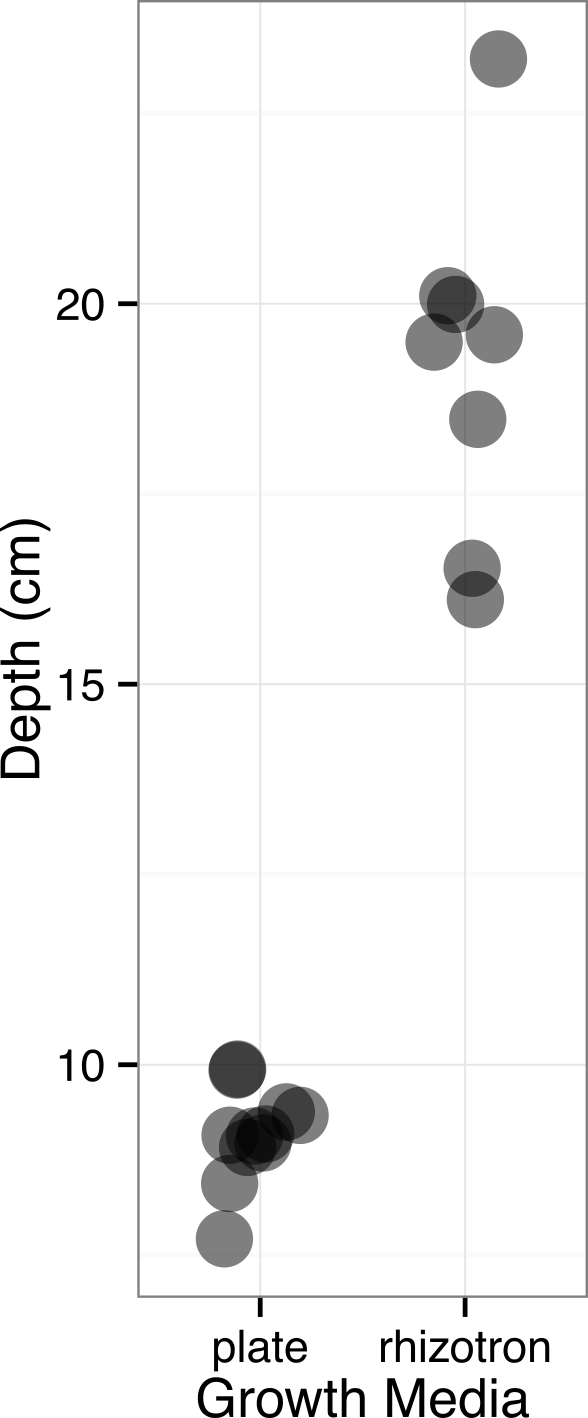
\includegraphics{/Users/rrellan/Dropbox/repos/GLO-Roots/figures/Supplements/Figure_4_figure_supplement_1.png}
\textbf{Figure 4-figure supplement 1}: ZAT12:LUC intensity and root
segments automatically idenfied values along the root tip. Data was
manually obtained by obtaining the intensity profile of the first 0.5 cm
from the root tip of individual lateral roots. Ten lateral roots for
each reporter were measured.\\\pagebreak

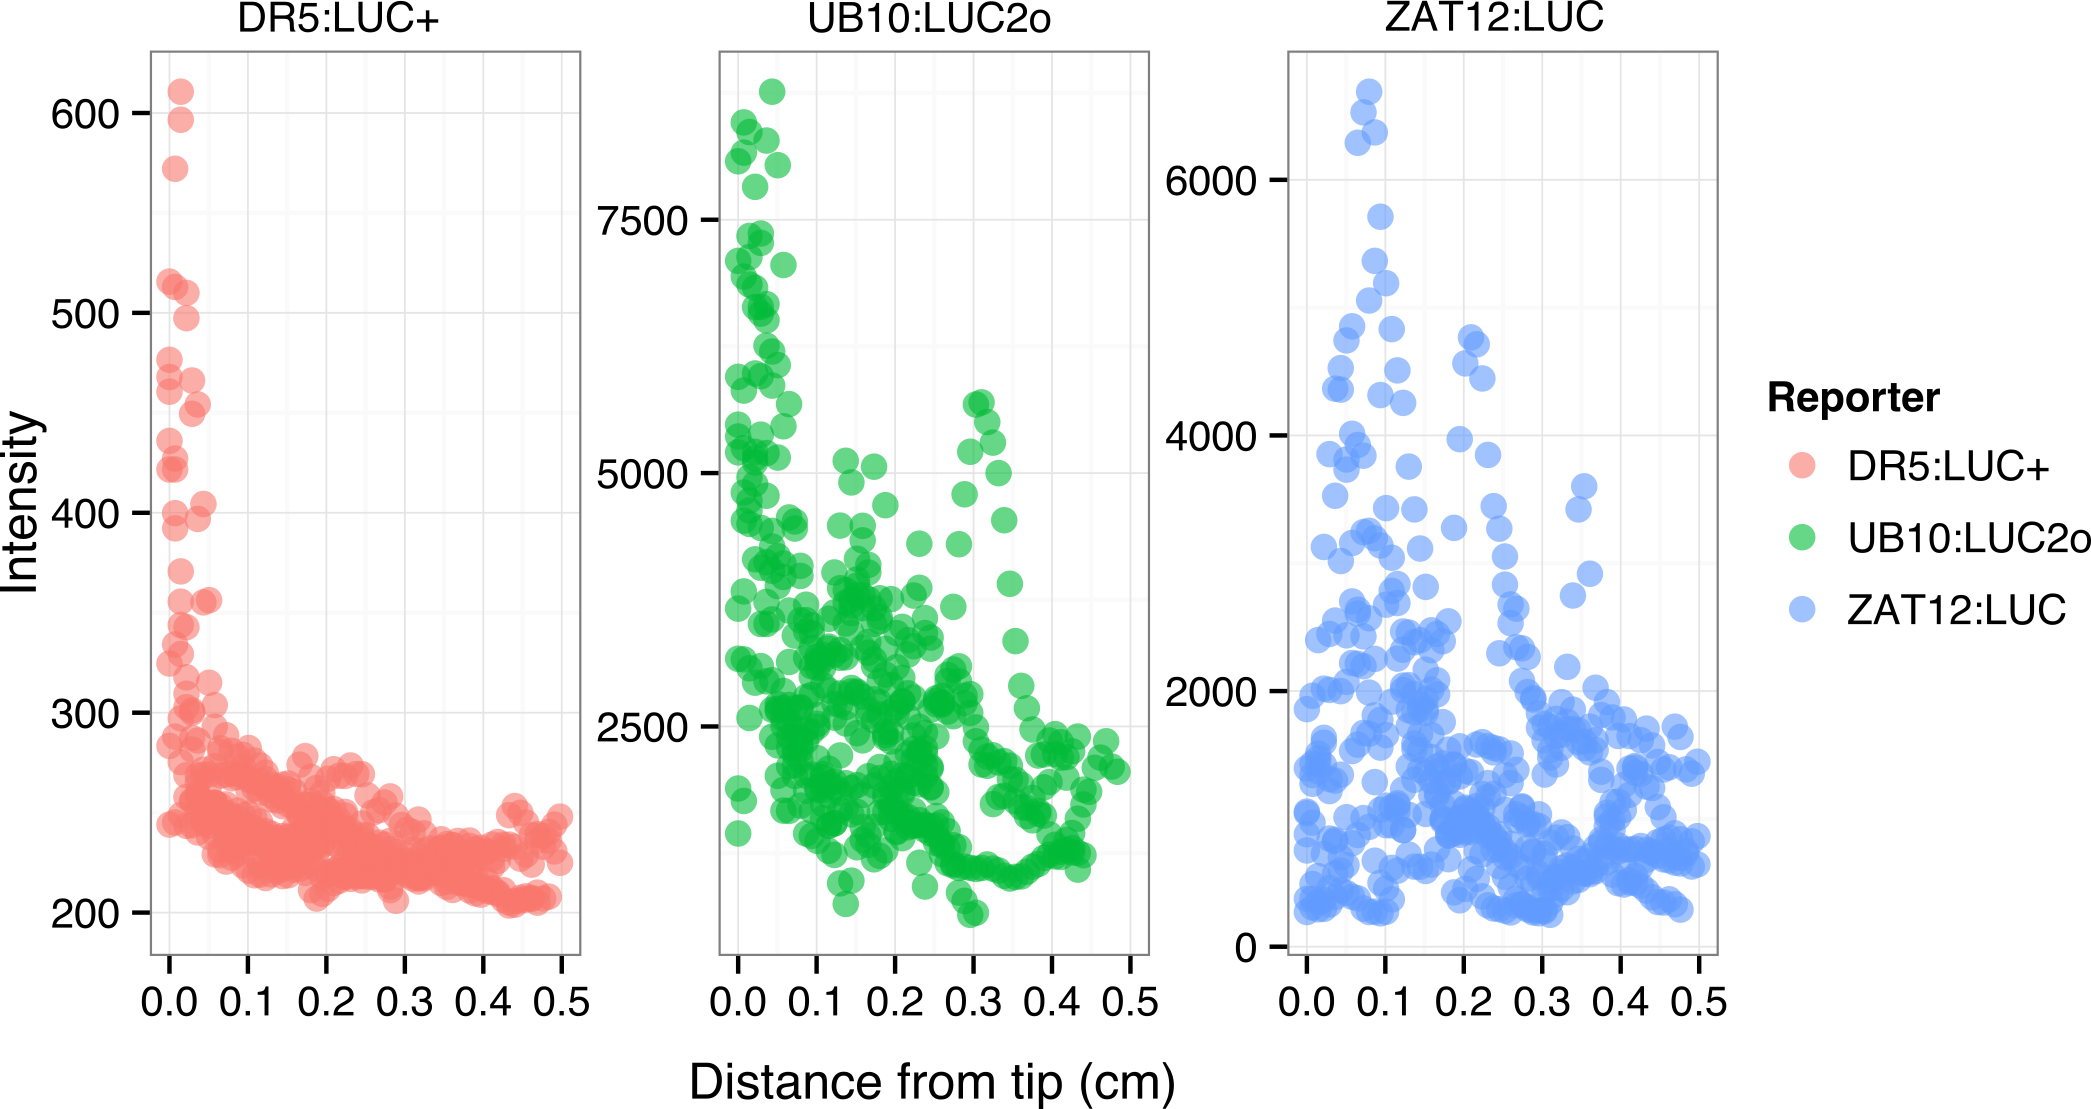
\includegraphics{/Users/rrellan/Dropbox/repos/GLO-Roots/figures/Supplements/Figure_4_figure_supplement_2.png}
\textbf{Figure 4-figure supplement 2}: DR5:LUC+, UBQ10:LUC2o and
ZAT12:LUC intensity values along the root tip. Data was manually
obtained by obtaining the intensity profile of the first 0.5 cm from the
root tip of individual lateral roots. Ten lateral roots for each
reporter were measured.\\\pagebreak

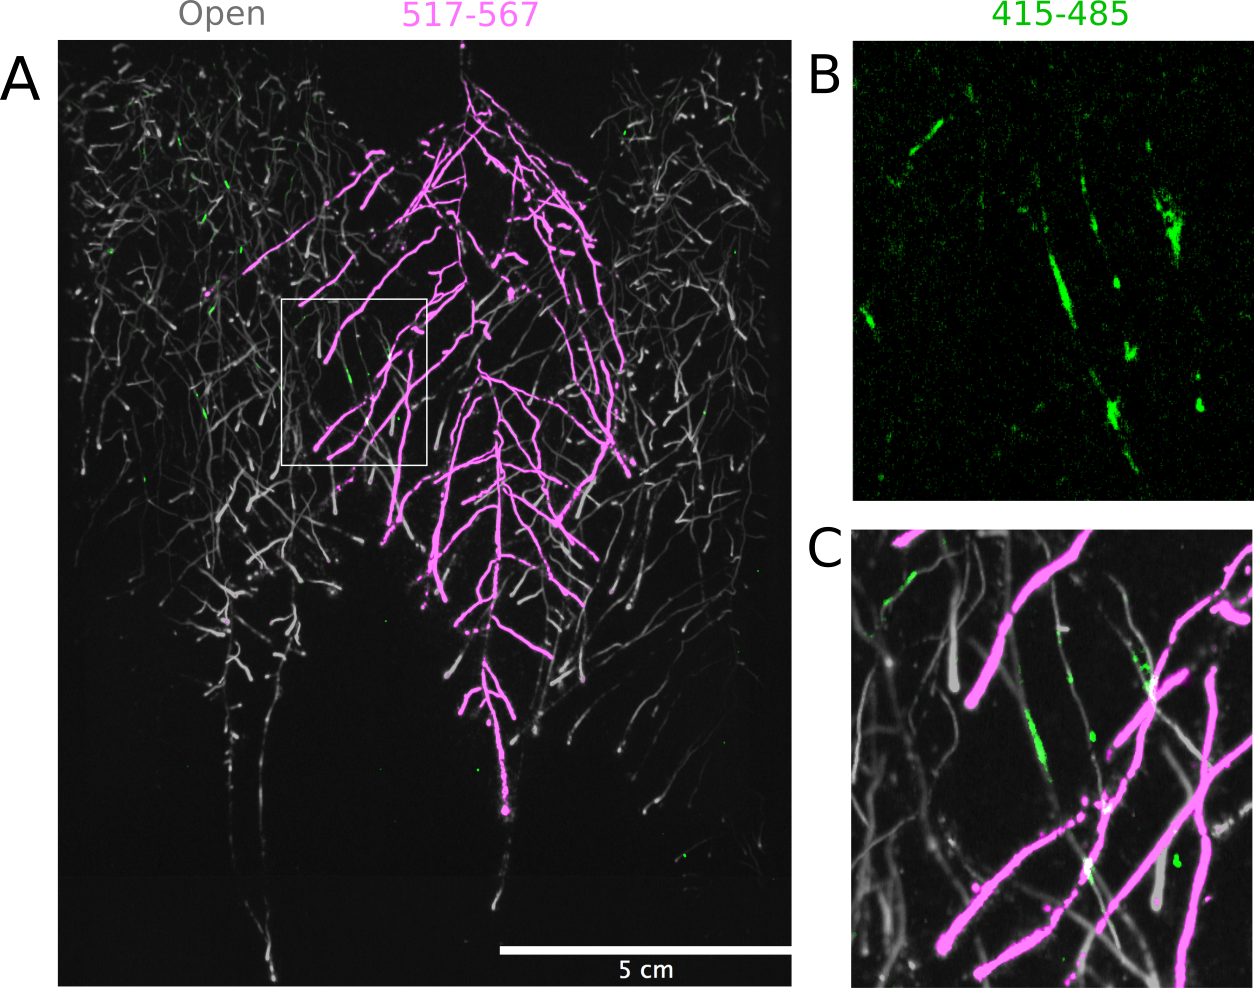
\includegraphics{/Users/rrellan/Dropbox/repos/GLO-Roots/figures/Supplements/Figure_4_figure_supplement_3.png}\\\textbf{Figure
4-figure supplement 3. Images of plants at 22 DAS growing in the same
rhizotron and expressing different luciferases.} A) Two Col-0 plants
expressing \emph{ProUBQ10:LUC2o} and \emph{ProACT2:PPyRE8o} B) Col-0
plant expressing \emph{ProACT2:PPyRE8o} and Sha plant expressing
\emph{ProUBQ10:LUC2o}.\\\pagebreak

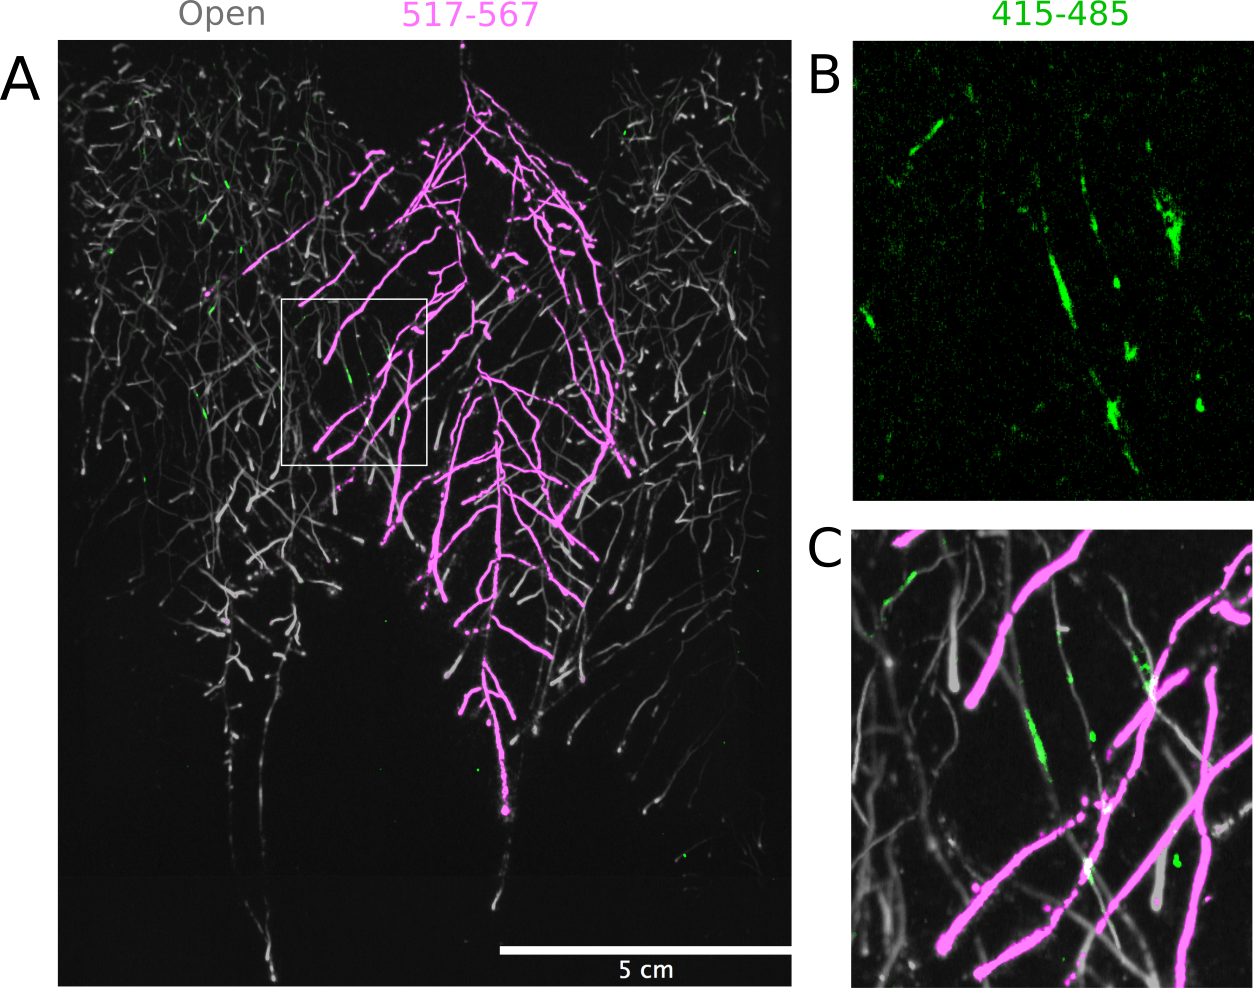
\includegraphics{/Users/rrellan/Dropbox/repos/GLO-Roots/figures/Supplements/Figure_4_figure_supplement_4.png}\\\textbf{Figure
4-figure supplement 4. Three-reporter-based analysis of
root-root-microbe interactions.} A) Image showing a 22 DAS
\emph{ProUBQ10:LUC2o} plant (magenta) grown in the same rhizotron with
\emph{ProACT2:PpyRE8o} plants (grey). Plants were inoculated with
\emph{Pseudomonas fluorescens CH267} (green). Magnified portion of root
systems colonized by \emph{Pseudomonas fluorescens} showing \emph{P.
fluorescences} (B) only or all three reporters together (C).\\\pagebreak

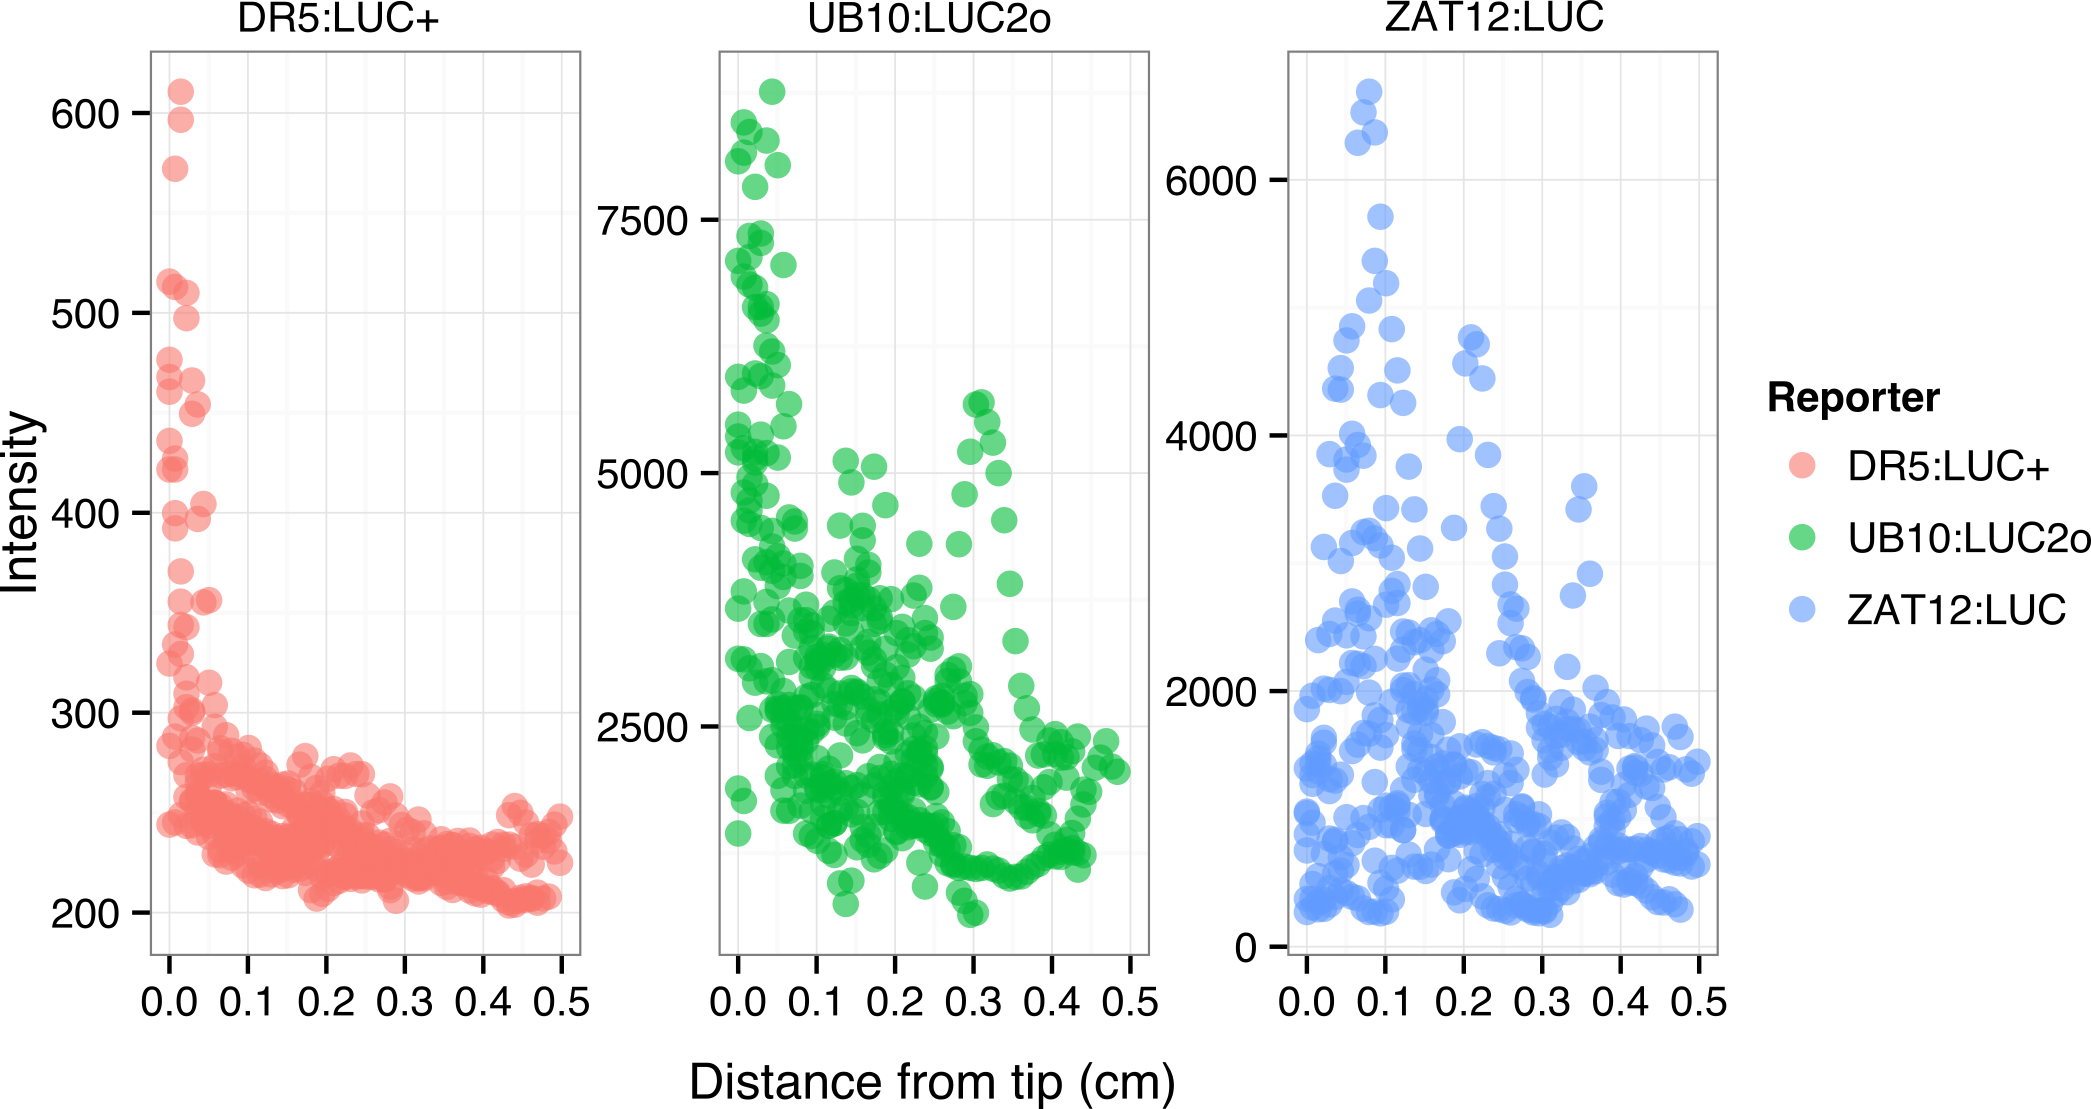
\includegraphics{/Users/rrellan/Dropbox/repos/GLO-Roots/figures/Supplements/Figure_5_figure_supplement_1.png}\\\textbf{Figure
5-figure supplement 1}: Moisture calibration curve. Rhizotrons with
different levels of moisture were prepared and scanned to obtain
readings of pixel intensity. Soil from rhizotrons was then weighed,
dried down in an oven at 70 ºC for 48 hours and percent water content
quantified.\\\pagebreak

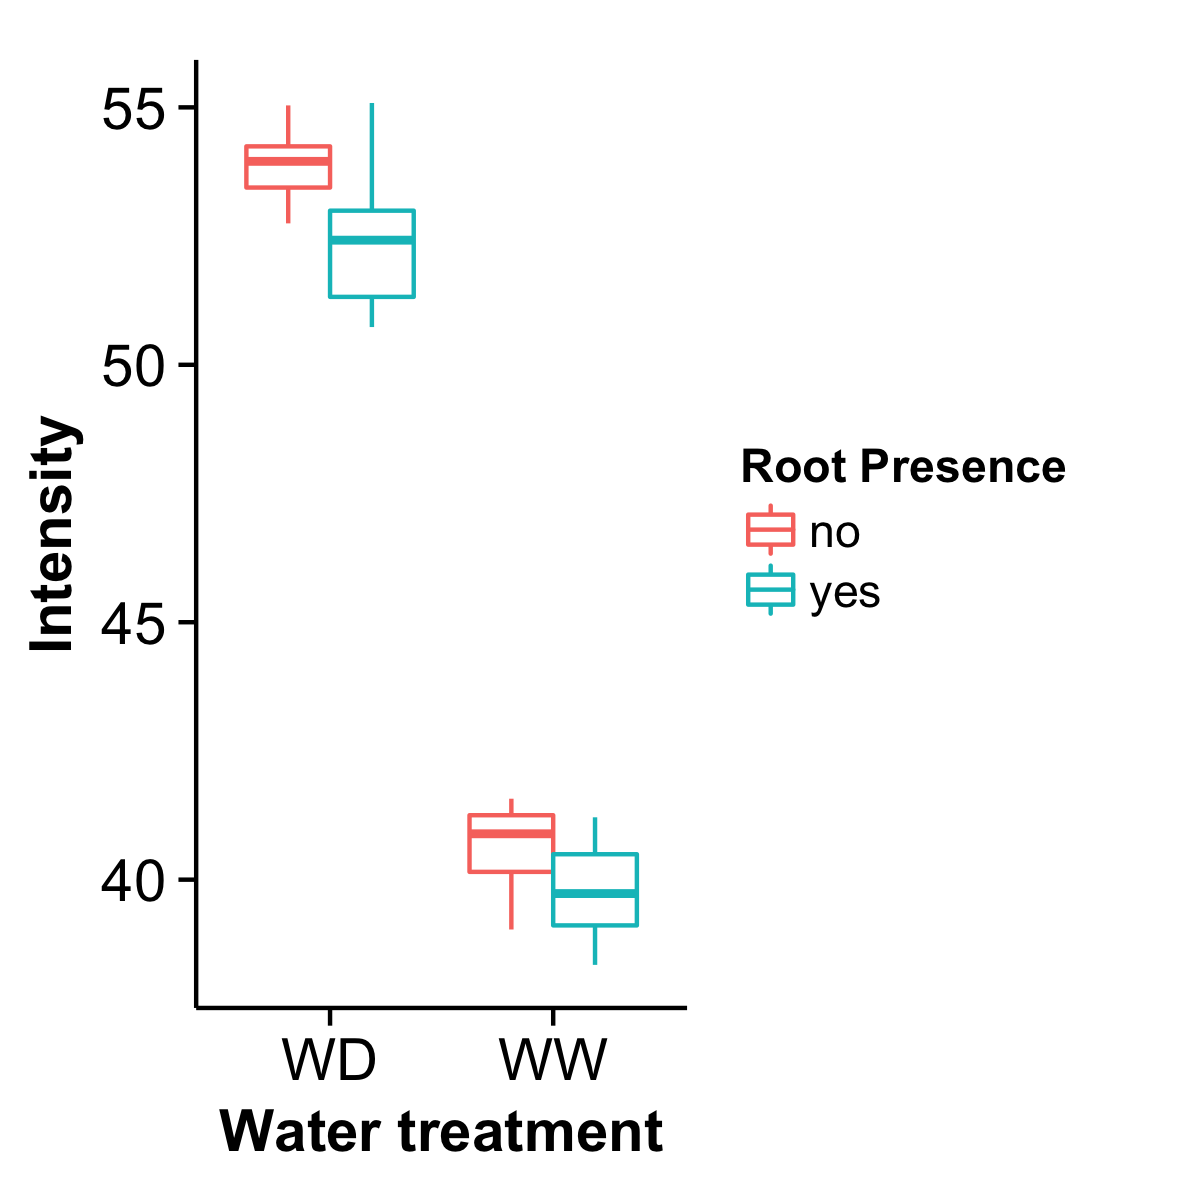
\includegraphics{/Users/rrellan/Dropbox/repos/GLO-Roots/figures/Supplements/Figure_5_figure_supplement_2.png}\\\textbf{Figure
5-figure supplement 2. Comparison of soil intensity values between areas
of the rhizotron with or without the presence of roots, determined based
on luminescence data.} Mean intensity values from 100 x 100 pixel
squares samples of both areas were obtained from 10 different
rhizotrons. Wilcoxon test analysis with p \textless{} 0.01 was used to
test significant differences between areas with our without root
presence.\\\pagebreak

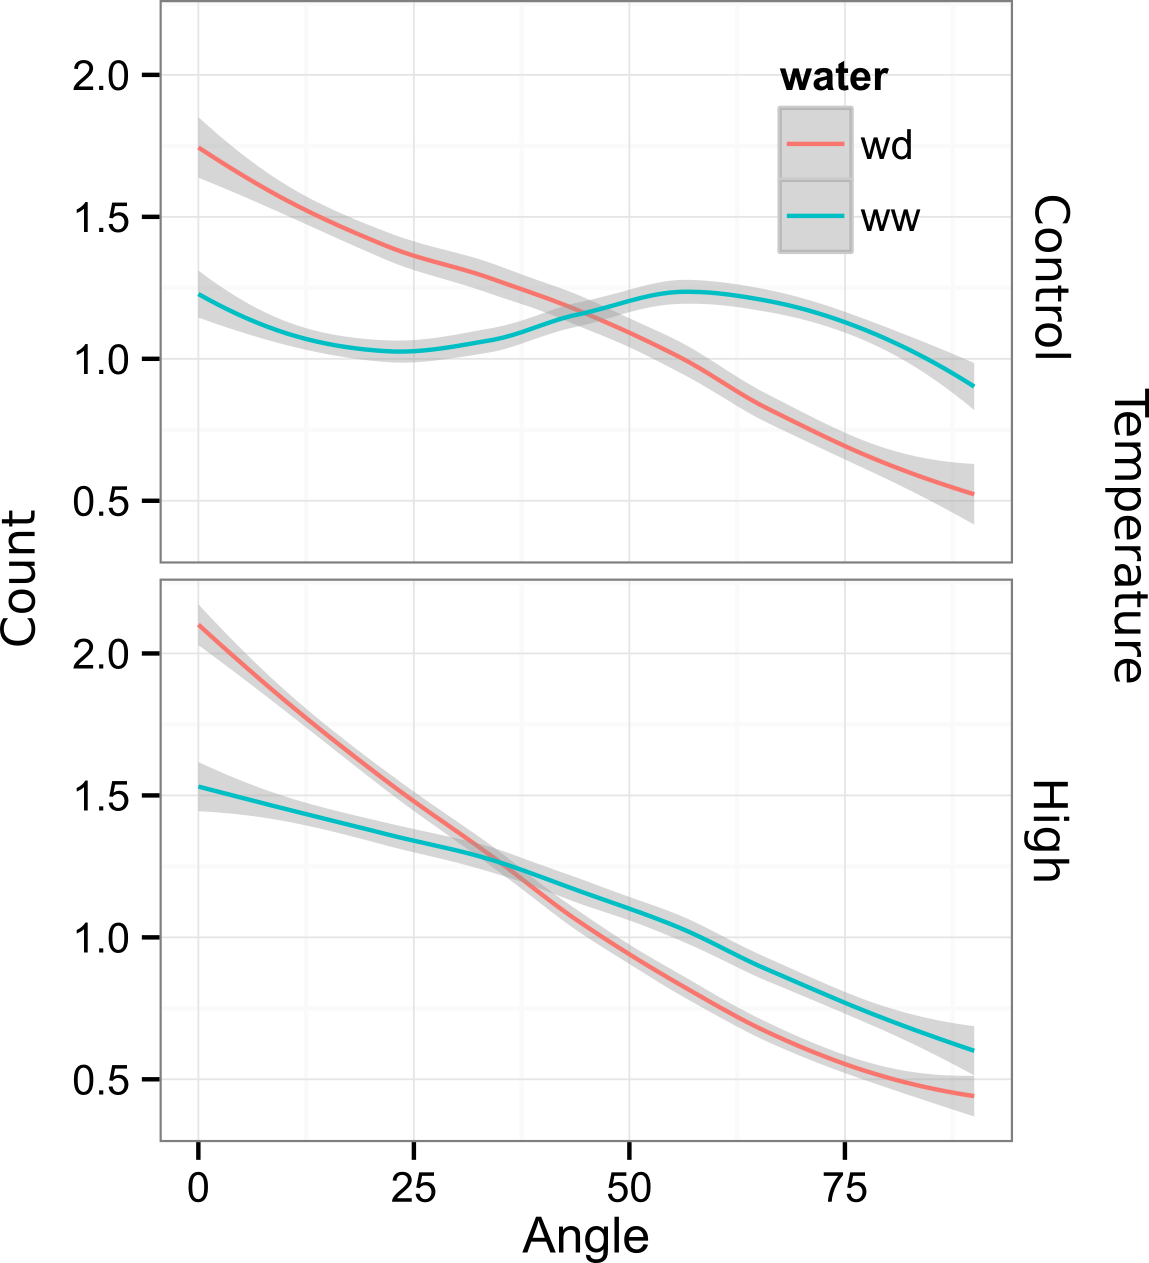
\includegraphics{/Users/rrellan/Dropbox/repos/GLO-Roots/figures/Supplements/Figure_6_figure_supplement_1.png}\\\textbf{Figure
6-figure supplement 1} Directionality analysis of roots of plants
transferred to water deprivation conditions after 9 DAS and kept 22 ºC
(control temperature) and 29 ºC (high temperature) until 22 DAS. (0º is
the direction of the gravity vector).\\\pagebreak

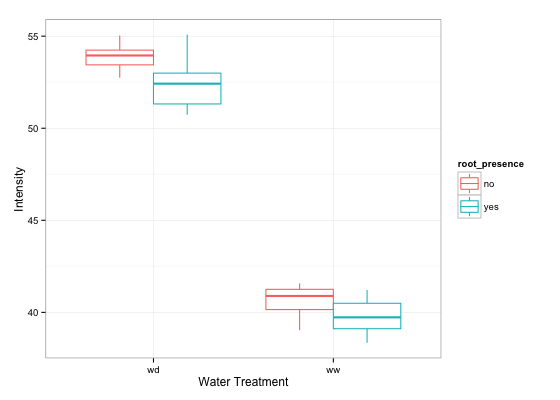
\includegraphics{/Users/rrellan/Dropbox/repos/GLO-Roots/figures/Supplements/Figure_6_figure_supplement_2.png}
\textbf{Figure 6-figure supplement 2. Phosphorus deficiency response of
root systems} Shoot and root systems of \emph{ProUBQ10:LUC2o} Col-0
plants growing in soil supplemented with 1ml of 100 µM P-Alumina (left)
and 0-P-Alumina (right) 22 (A) or 27 (B) DAS. C) Root depth/width ratio
of 22 (top) and 27 (bottom) DAS plants. D) Scatter-plot showing
relationship between root and shoot system area at 22 (top) and 27
(bottom) DAS. E) Root directionality distribution in plants 22 (top) and
27 (bottom) DAS. Anova analysis at p \textless{} 0.01 was used to
compare depth/width ratios in P treatments. Kolmogorov-Smirnov test at p
\textless{} 0.001 was used to compare directionality distributions
between the different treatments. A Local Polynomial Regression Fitting
with 95\% confidence interval (grey) was used to represent the
directionality distribution curve.(0º is the direction of the gravity
vector).\\\pagebreak

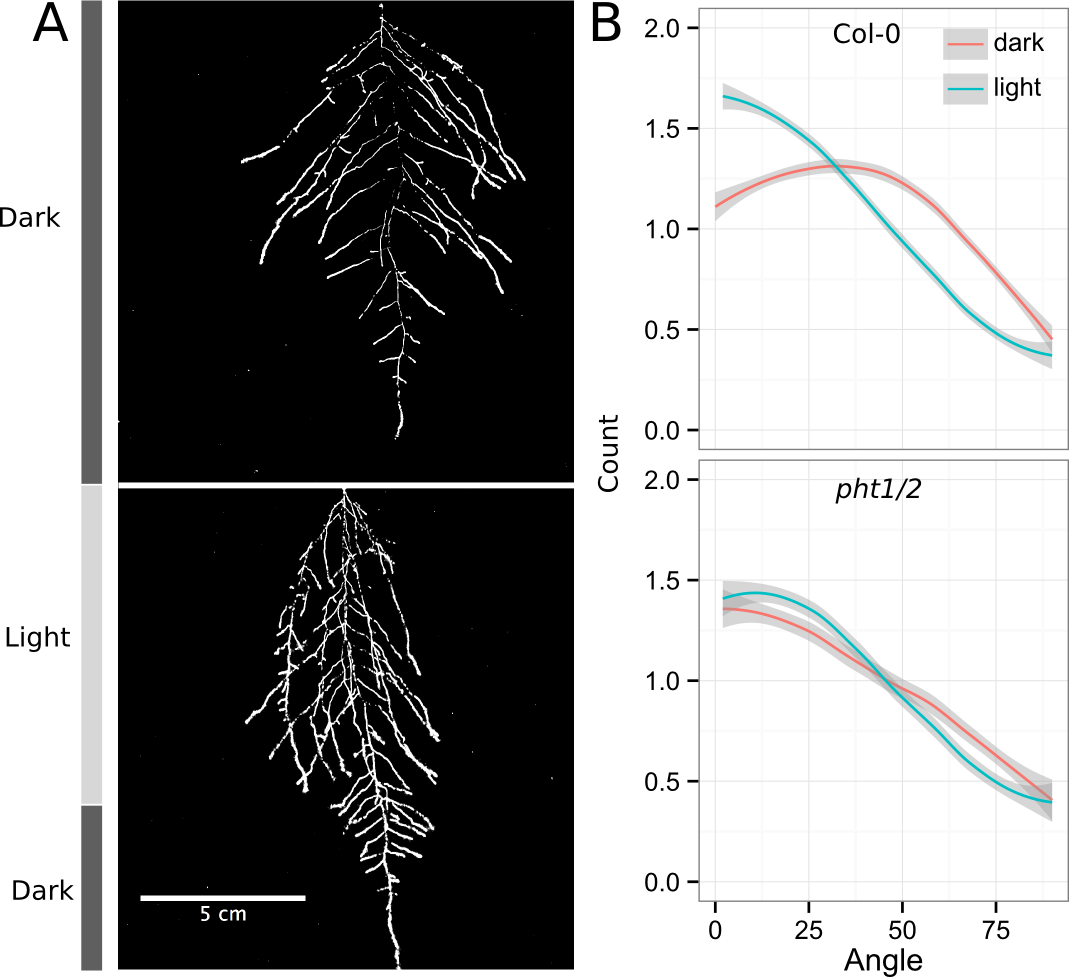
\includegraphics{/Users/rrellan/Dropbox/repos/GLO-Roots/figures/Supplements/Figure_6_figure_supplement_3.png}\\\textbf{Figure
6-figure supplement 3. Effect of light on root directionality.} A) Col-0
root systems shielded (top) or light exposed (bottom). After 9 DAS the
top third of the rhizotron was exposed to light (indicated on the side
with a light grey bar) and plants were imaged at 20 DAS. B)
Directionality analysis of root systems shielded (red) or exposed
(green) to light for Col-0 (top panel) or \emph{phot1/2} double mutant
(bottom panel). Between 4 and 6 plants were analyzed per treatment.
ANOVA analysis at p \textless{} 0.01 was used to compare depth/width
ratios in P treatments. Kolmogorov-Smirnov test at p \textless{} 0.001
was used to compare directionality distributions between the different
treatments. A Local Polynomial Regression Fitting with 95\% confidence
interval (grey) was used to represent the directionality distribution
curve.(0º is the direction of the gravity vector). \pagebreak

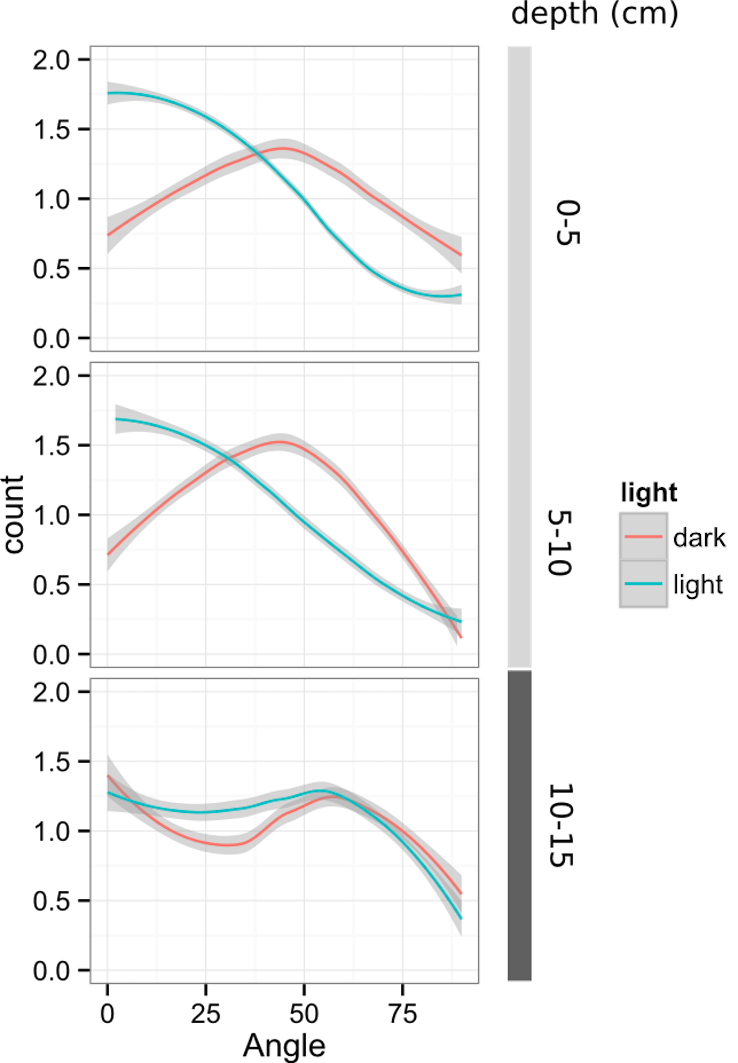
\includegraphics{/Users/rrellan/Dropbox/repos/GLO-Roots/figures/Supplements/Figure_6_figure_supplement_4.png}\\\textbf{Figure
6-figure supplement 4} Plots showing output of directionality analysis
performed at different depths (0-5, 5-10, 10-15 cm) in rhizotrons
exposed to light or kept in the dark. (0º is the direction of the
gravity vector).\\\pagebreak

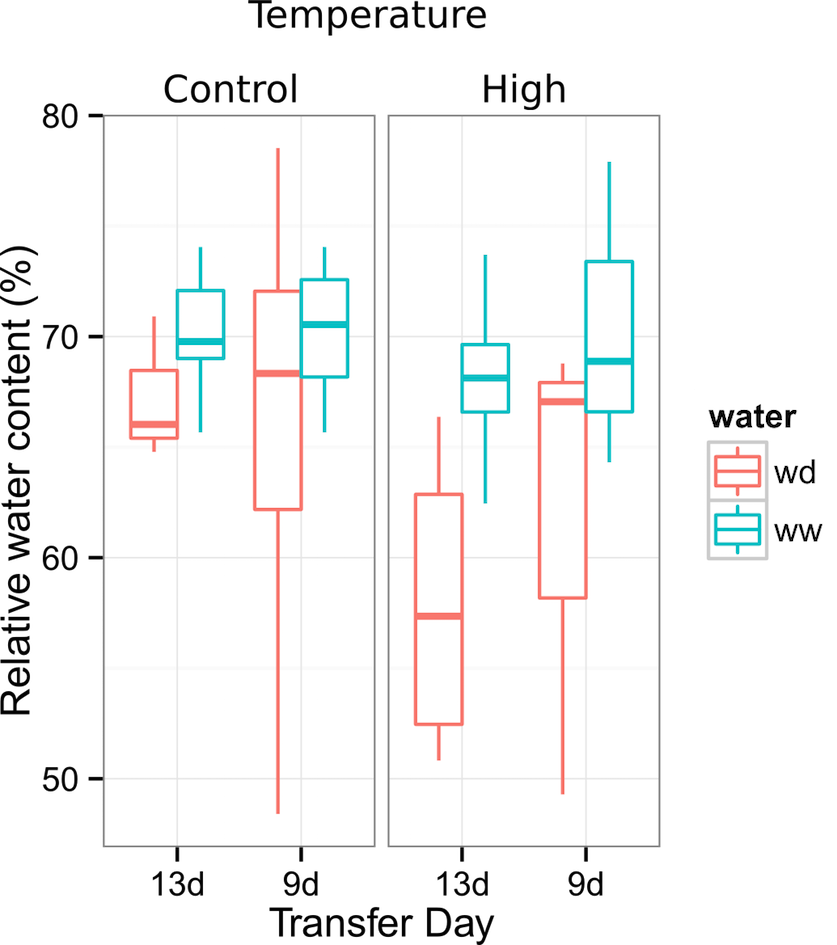
\includegraphics{/Users/rrellan/Dropbox/repos/GLO-Roots/figures/Supplements/Figure_6_figure_supplement_5.png}\\\textbf{Figure
6-figure supplement 5. Leaf relative water content of 23 DAS plants that
were subjected to water deprivation (WD) after 9 or 13 DAS or kept under
well watered (WD) conditions.} At 9 DAS half of the plants were kept
under control temperature conditions (22 ºC) and the other half
transferred to a 29 ºC (high) chamber. n = 6-8 plants.\\\pagebreak

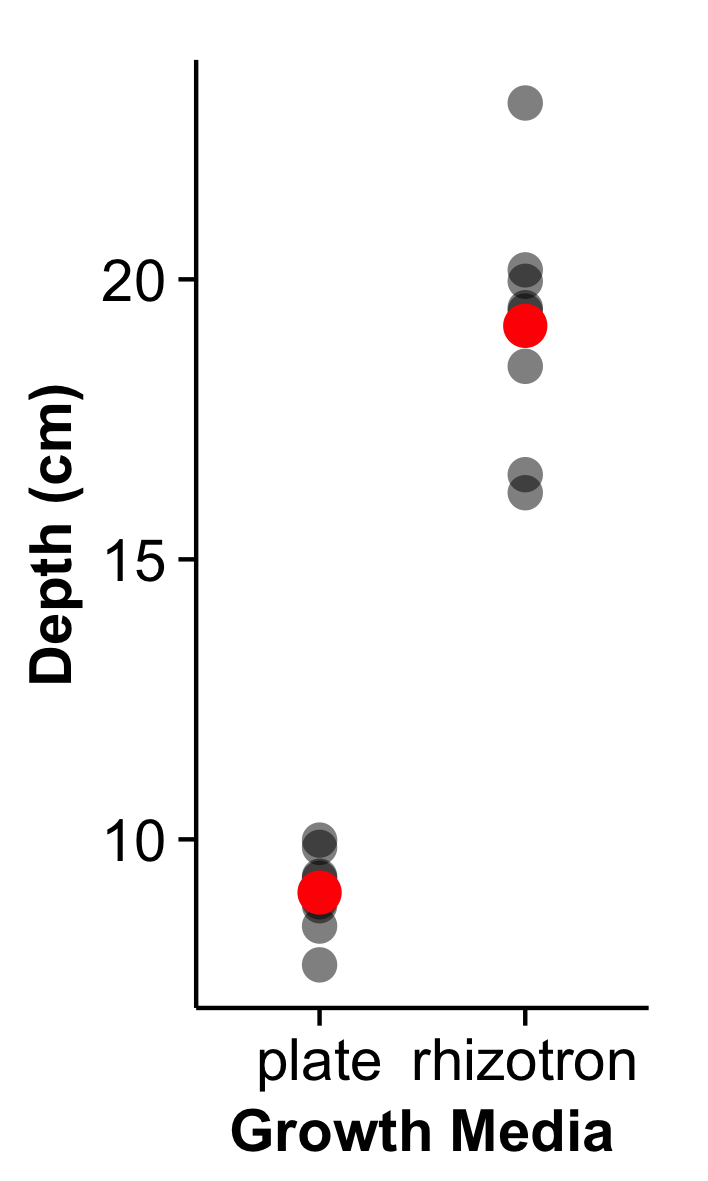
\includegraphics{/Users/rrellan/Dropbox/repos/GLO-Roots/figures/Supplements/Figure_8_figure_supplement_1.png}\\\textbf{Figure
8-figure supplement 1} Depth of the primary root of Brachypodium plants
grown in rhizotrons or on gel-based media (n=8-11).\\\pagebreak

\subsubsection{Supplementary material}\label{supplementary-material-1}

\textbf{\href{https://www.dropbox.com/s/f01cg10hqehpnv6/supplement_1.zip?dl=0}{Supplemental
Material 1}}\\Blueprints of the holders, clear sheets and spacers needed
to built the rhizotrons. Additional details are provided in the
materials and methods. Files are provided in Adobe Illustrator .ai and
Autocad .dxf formats.

\textbf{\href{https://www.dropbox.com/s/hn1hhuttdby7y0j/supplement_2.csv?dl=0}{Supplemental
Material 2}}\\Primers used in the qPCR
experiment.\\\textbf{\href{https://www.dropbox.com/s/kg0r5df4nx3tjpy/supplement_3.zip?dl=0}{Supplemental
Material 3}}\\Vector maps of all the constructs used in this work.

\subsection{Source data files}\label{source-data-files}

Source data files used for building the following figures are provided:
figure\_1D.csv\\figure\_1\_figure\_supplement\_1A-B.csv\\figure\_1\_figure\_supplement\_1C\_D.csv\\figure\_1\_figure\_supplement\_1E-F.csv\\figure\_1\_figure\_supplement\_2.csv\\figure\_1\_figure\_supplement\_3.csv\\figure\_2C.csv\\figure\_2D.csv\\figure\_3D.csv\\figure\_3E.csv\\figure\_3F-G\_1.csv\\figure\_3F-G\_2.tps\\figure\_3\_figure\_supplement\_1A-B.csv\\figure\_4G\_reporter.csv\\figure\_4G\_root\_segment.csv\\figure\_4\_figure\_supplement\_1.csv\\figure\_4\_figure\_supplement\_2.csv\\figure\_5\_figure\_supplement\_1.csv\\figure\_6\_A-D.csv\\figure\_6\_figure\_supplement\_2-C-D.csv\\figure\_6\_figure\_supplement\_2-E.csv\\figure\_6\_figure\_supplement\_3.csv\\figure\_6\_figure\_supplement\_4.csv\\figure\_6\_figure\_supplement\_5.csv\\figure\_7.csv\\figure\_8\_figure\_supplement\_1.csv

\pagebreak

\subsection*{References}\label{references}
\addcontentsline{toc}{subsection}{References}

1.Dinneny, J. R. \emph{et al.} Cell identity mediates the response of
\emph{Arabidopsis} roots to abiotic stress. \emph{Science} \textbf{320,}
942--945 (2008).

2.Duan, L. \emph{et al.} Endodermal ABA Signaling Promotes Lateral Root
Quiescence during Salt Stress in Arabidopsis Seedlings. \emph{Plant
Cell} \textbf{25,} 324--341 (2013).

3.Lynch, J. P. \& Wojciechowski, T. Opportunities and challenges in the
subsoil: pathways to deeper rooted crops. \emph{J. Exp. Bot.}
\textbf{66,} 2199--2210 (2015).

4.Brady, N. C. \& Weil, R. R. \emph{Elements of the nature and
properties of soils}. (Prentice Hall, 2009).

5.Bao, Y. \emph{et al.} Plant roots use a patterning mechanism to
position lateral root branches toward available water. \emph{Proc Natl
Acad Sci} \textbf{111,} 9319--9324 (2014).

6.Tabata, R. \emph{et al.} Perception of root-derived peptides by shoot
LRR-RKs mediates systemic N-demand signaling. \emph{Science}
\textbf{346,} 343--346 (2014).

7.Rosquete, M. R. \emph{et al.} An Auxin Transport Mechanism Restricts
Positive Orthogravitropism in Lateral Roots. \emph{Current Biology}
\textbf{23,} 817--822 (2013).

8.Uga, Y. \emph{et al.} Control of root system architecture by DEEPER
ROOTING 1 increases rice yield under drought conditions. \emph{Nat.
Genet.} \textbf{45,} 1097--1102 (2013).

9.Postma, J. A. \& Lynch, J. P. The optimal lateral root branching
density for maize depends on nitrogen and phosphorus availability.
\emph{Plant Physiol.} \textbf{166,} 590--602 (2014).

10.Schneider, C. A., Rasband, W. S. \& Eliceiri, K. W. NIH Image to
ImageJ: 25 years of image analysis. \emph{Nature methods} \textbf{9,}
671--675 (2012).

11.Meijon, M., Satbhai, S. B., Tsuchimatsu, T. \& Busch, W. Genome-wide
association study using cellular traits identifies a new regulator of
root development in. \emph{Nat. Genet.} \textbf{46,} 77--81 (2013).

12.Hara-Miyauchi, C. \emph{et al.} Bioluminescent system for dynamic
imaging of cell and animal behavior. \emph{Biochem. Biophys. Res.
Commun.} \textbf{419,} 188--193 (2012).

13.Emami, S., Yee, M.-C. \& Dinneny, J. R. A robust family of Golden
Gate Agrobacterium vectors for plant synthetic biology. \emph{Front.
Plant Sc.} \textbf{4,} 339 (2013).

14.Hall, M. P. \emph{et al.} Engineered Luciferase Reporter from a Deep
Sea Shrimp Utilizing a Novel Imidazopyrazinone Substrate. \emph{ACS
chemical biology} \textbf{7,} 1848--1857 (2012).

15.Ristova, D. \emph{et al.} RootScape: a landmark-based system for
rapid screening of root architecture in Arabidopsis. \emph{Plant
Physiology} \textbf{161,} 1086--1096 (2013).

16.Lobet, G. \emph{et al.} Root System Markup Language: toward a unified
root architecture description language. \emph{Plant Physiol.}
\textbf{167,} 617--627 (2015).

17.Pag{è}s, L. \emph{et al.} Calibration and evaluation of ArchiSimple,
a simple model of root system architecture. \emph{Ecological Modelling}
\textbf{290,} 76--84 (2014).

18.Moreno-Risueno, M. A. \emph{et al.} Oscillating gene expression
determines competence for periodic \emph{Arabidopsis} root branching.
\emph{Science} \textbf{329,} 1306--1311 (2010).

19.Miller, G. \emph{et al.} The plant NADPH oxidase RBOHD mediates rapid
systemic signaling in response to diverse stimuli. \emph{Science
Signaling} \textbf{2,} ra45 (2009).

20.Haney, C. H., Samuel, B. S., Bush, J. \& Ausubel, F. M. Associations
with rhizosphere bacteria can confer an adaptive advantage to plants.
\emph{Nature Plants} \textbf{1,} 15051 (2015).

21.Mandoli, D. F., FORD, G. A., WALDRON, L. J., NEMSON, J. A. \& Briggs,
W. R. Some spectral properties of several soil types: implications for
photomorphogenesis*. \emph{Plant Cell Environ.} \textbf{13,} 287--294
(1990).

22.Galen, C., Rabenold, J. J. \& Liscum, E. Functional ecology of a blue
light photoreceptor: effects of phototropin-1 on root growth enhance
drought tolerance in Arabidopsis thaliana. \emph{New Phytol.}
\textbf{173,} 91--99 (2007).

23.Moni, A., Lee, A. Y., Briggs, W. R. \& Han, I. S. The blue light
receptor Phototropin 1 suppresses lateral root growth by controlling
cell elongation. \emph{Plant Biology} 34--40 (2014).

24.Yokawa, K., Kagenishi, T. \& Balu{š}ka, F. Root photomorphogenesis in
laboratory-maintained Arabidopsis seedlings. \emph{Trends Plant Sci.}
\textbf{18,} 117--119 (2013).

25.Lobell, D. B. \emph{et al.} Greater Sensitivity to Drought
Accompanies Maize Yield Increase in the U.S. Midwest. \emph{Science}
\textbf{344,} 516--519 (2014).

26.Ort, D. R. \& Long, S. P. Limits on Yields in the Corn Belt.
\emph{Science} \textbf{344,} 484--485 (2014).

27.Pacheco-Villalobos, D. \& Hardtke, C. S. Natural genetic variation of
root system architecture from Arabidopsis to Brachypodium: towards
adaptive value. \emph{Philosophical Transactions of the Royal Society of
London B: Biological Sciences} \textbf{367,} 1552--1558 (2012).

28.Watt, M., Schneebeli, K., Dong, P. \& Wilson, I. W. The shoot and
root growth of Brachypodium and its potential as a model for wheat and
other cereal crops. \emph{Functional Plant Biol.} \textbf{36,} 960--969
(2009).

29.Mann, D. G. J. \emph{et al.} Gateway-compatible vectors for
high-throughput gene functional analysis in switchgrass (Panicum
virgatum L.) and other monocot species. \emph{Plant Biotechnol. J.}
\textbf{10,} 226--236 (2012).

30.Pacheco-Villalobos, D., Sankar, M., Ljung, K. \& Hardtke, C. S.
Disturbed Local Auxin Homeostasis Enhances Cellular Anisotropy and
Reveals Alternative Wiring of Auxin-ethylene Crosstalk in Brachypodium
distachyon Seminal Roots. \emph{PLoS Genet} \textbf{9,} e1003564 (2013).

31.Buer, C. S., Wasteneys, G. O. \& Masle, J. Ethylene modulates
root-wave responses in Arabidopsis. \emph{Plant Physiology}
\textbf{132,} 1085--1096 (2003).

32.Blossfeld, S., Schreiber, C. M., Liebsch, G., Kuhn, A. J. \&
Hinsinger, P. Quantitative imaging of rhizosphere pH and CO2 dynamics
with planar optodes. \emph{Annals of Botany} \textbf{112,} 267--276
(2013).

33.Shaw, S. L. \& Ehrhardt, D. W. Smaller, Faster, Brighter: Advances in
Optical Imaging of Living Plant Cells. \emph{Annu. Rev. Plant Biol.}
\textbf{64,} 351--375 (2013).

34.Barr, H. \& Weatherley, P. A re-examination of the relative turgidity
technique for estimating water deficit in leaves. \emph{Aust. J. Biol.
Sci} \textbf{15,} 413--428 (1962).

35.Grapov, D. DeviumWeb: Dynamic Multivariate Data Analysis and
Visualization Platform.

36.Branchini, B. R. \emph{et al.} Red-emitting luciferases for
bioluminescence reporter and imaging applications. \emph{Analytical
Biochemistry} \textbf{396,} 290--297 (2010).

37.Branchini, B. R. \emph{et al.} Thermostable red and green
light-producing firefly luciferase mutants for bioluminescent reporter
applications. \emph{Analytical Biochemistry} \textbf{361,} 253--262
(2007).

38.Lane, M. C., Alteri, C. J., Smith, S. N. \& Mobley, H. L. T.
Expression of flagella is coincident with uropathogenic Escherichia coli
ascension to the upper urinary tract. \emph{Proc. Natl. Acad. Sci.
U.S.A.} \textbf{104,} 16669--16674 (2007).

39.Ruegger, M. \emph{et al.} The TIR1 protein of Arabidopsis functions
in auxin response and is related to human SKP2 and yeast grr1p.
\emph{Genes Dev} \textbf{12,} 198--207 (1998).

40.Moriwaki, T. \emph{et al.} Hormonal Regulation of Lateral Root
Development in Arabidopsis Modulated by MIZ1 and Requirement of GNOM
Activity for MIZ1 Function. \emph{Plant Physiol.} \textbf{157,}
1209--1220 (2011).

41.Vogel, J. \& Hill, T. High-efficiency Agrobacterium-mediated
transformation of Brachypodium distachyon inbred line Bd21-3.
\emph{Plant Cell Rep} \textbf{27,} 471--478 (2008).

42.Covington, M. F. \& Harmer, S. L. The Circadian Clock Regulates Auxin
Signaling and Responses in Arabidopsis. \emph{Plos Biol} \textbf{5,}
e222 (2007).

43.Lindeboom, J. J. \emph{et al.} A Mechanism for Reorientation of
Cortical Microtubule Arrays Driven by Microtubule Severing.
\emph{Science} \textbf{342,} 1245533--1--1245533--11 (2013).

44.Chitwood, D. H. \emph{et al.} A modern ampelography: a genetic basis
for leaf shape and venation patterning in grape. \emph{Plant Physiology}
\textbf{164,} 259--272 (2014).

45.Iwata, H. \& Ukai, Y. SHAPE: a computer program package for
quantitative evaluation of biological shapes based on elliptic Fourier
descriptors. \emph{The Journal of Heredity} \textbf{93,} 384--385
(2002).

46.R Core Team. \emph{R: A language and environment for statistical
computing}. (R Foundation for Statistical Computing, 2014). at
\textless{}\url{http://www.R-project.org/}\textgreater{}

47.Wickham, H. \emph{Tidyr: Easily tidy data with spread() and gather()
functions.} (2014). at
\textless{}\url{http://CRAN.R-project.org/package=tidyr}\textgreater{}

48.Auguie, B. \emph{GridExtra: Functions in grid graphics}. (2012). at
\textless{}\url{http://CRAN.R-project.org/package=gridExtra}\textgreater{}

49.Dryden, I. L. \emph{Shapes: Statistical shape analysis}. (2013). at
\textless{}\url{http://CRAN.R-project.org/package=shapes}\textgreater{}

50.Adams, D. \& Otarola-Castillo, E. Geomorph: An r package for the
collection and analysis of geometric morphometric shape data.
\emph{Methods in Ecology and Evolution} \textbf{4,} 393--399 (2013).

51.Wickham, H. \emph{Ggplot2: Elegant graphics for data analysis}.
(Springer New York, 2009). at
\textless{}\url{http://had.co.nz/ggplot2/book}\textgreater{}

52.Wilke, C. O. \emph{cowplot: Streamlined Plot Theme and Plot
Annotations for ggplot2}. (2015). at
\textless{}\url{http://cran.r-project.org/web/packages/cowplot/index.html}\textgreater{}

\end{document}
